\documentclass[12pt]{article}

\usepackage[left=1in,right=1in,top=1in,bottom=1in]{geometry}
\usepackage{graphicx}
\usepackage{tikz}
\usepackage{booktabs}
\usepackage{makecell} 

\usepackage[dvipsnames]{xcolor}
\definecolor{csub-blue}{RGB}{0, 53, 148}
\usepackage[unicode,hyperfootnotes=true,linktocpage,pagebackref]{hyperref}
 \hypersetup{%
   colorlinks = true,
   pdfborder = {0 0 0},
   citecolor = csub-blue,
   linkcolor = csub-blue,
   urlcolor  = csub-blue,
 }%
\urlstyle{same}


% \makeatletter
% \def\@fnsymbol#1{\ensuremath{\ifcase#1\or *\or \mathsection\or \mathparagraph\or \|\or **\or \dagger\dagger \or \ddagger\ddagger \else\@ctrerr\fi}}
% \makeatother

\title{Tables and Figures for \\
  \textsf{\Large Employment, Input--Output Linkages, and the\\Energy Transition in California's Top Oil-Producing Region}}
\author{Rich Ryan\thanks{Email: \href{mailto:richryan@csub.edu}{richryan@csub.edu}. Department of Economics, California State University, Bakersfield.}} 

\date{May 29, 2026}

\begin{document}
\maketitle

\section{Figures}

\begin{figure}[htbp]
  \centering
  % \resizebox{<horizontal size>}{<vertical size>}{%
  \resizebox{\textwidth}{!}{
  % Created by tikzDevice version 0.12.6 on 2026-02-22 21:41:52
% !TEX encoding = UTF-8 Unicode
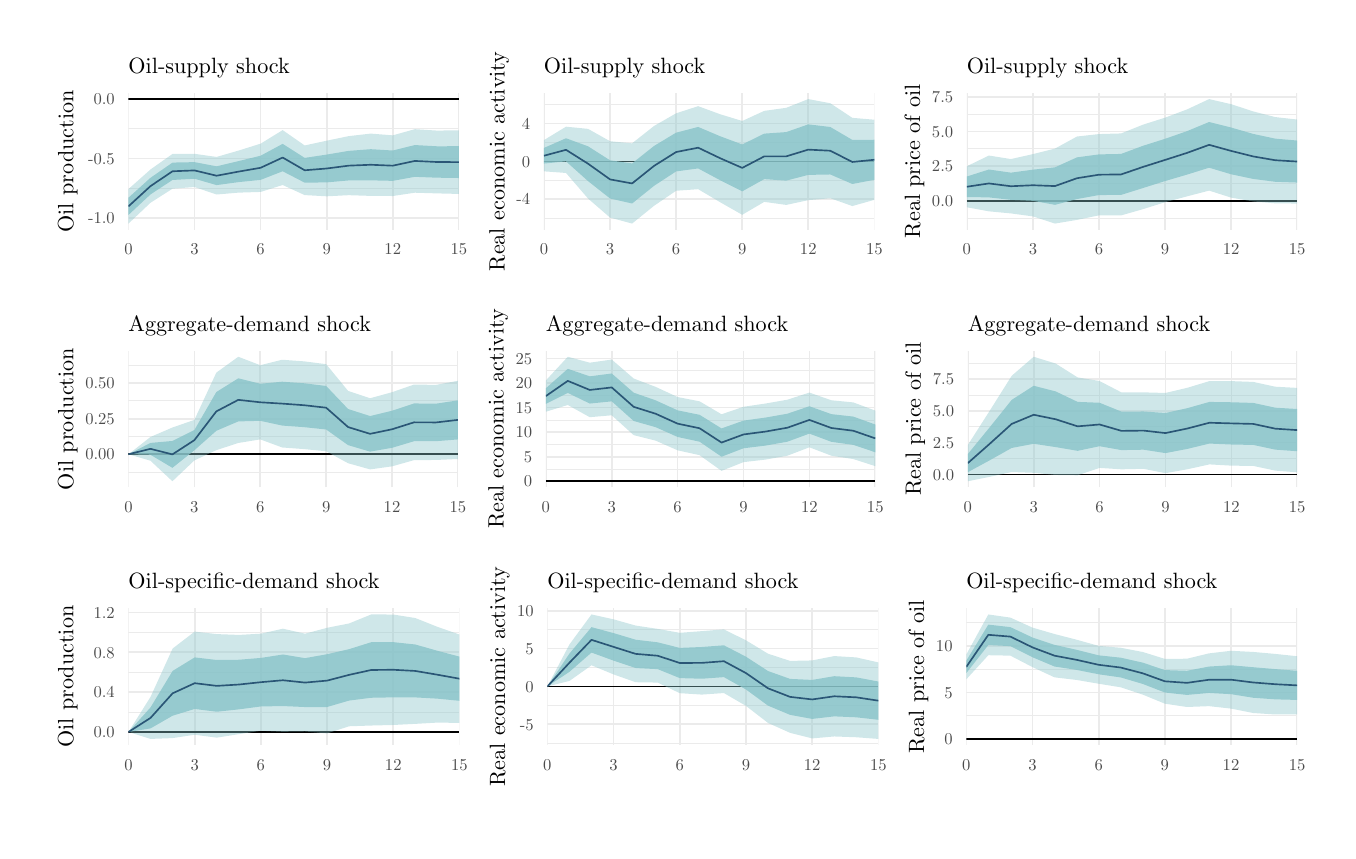
\begin{tikzpicture}[x=1pt,y=1pt]
\definecolor{fillColor}{RGB}{255,255,255}
\path[use as bounding box,fill=fillColor,fill opacity=0.00] (0,0) rectangle (469.75,290.32);
\begin{scope}
\path[clip] ( 36.43,217.28) rectangle (155.81,266.76);
\definecolor{drawColor}{gray}{0.92}

\path[draw=drawColor,line width= 0.3pt,line join=round] ( 36.43,232.29) --
	(155.81,232.29);

\path[draw=drawColor,line width= 0.3pt,line join=round] ( 36.43,253.77) --
	(155.81,253.77);

\path[draw=drawColor,line width= 0.6pt,line join=round] ( 36.43,221.55) --
	(155.81,221.55);

\path[draw=drawColor,line width= 0.6pt,line join=round] ( 36.43,243.03) --
	(155.81,243.03);

\path[draw=drawColor,line width= 0.6pt,line join=round] ( 36.43,264.51) --
	(155.81,264.51);

\path[draw=drawColor,line width= 0.6pt,line join=round] ( 36.43,217.28) --
	( 36.43,266.76);

\path[draw=drawColor,line width= 0.6pt,line join=round] ( 60.30,217.28) --
	( 60.30,266.76);

\path[draw=drawColor,line width= 0.6pt,line join=round] ( 84.18,217.28) --
	( 84.18,266.76);

\path[draw=drawColor,line width= 0.6pt,line join=round] (108.06,217.28) --
	(108.06,266.76);

\path[draw=drawColor,line width= 0.6pt,line join=round] (131.93,217.28) --
	(131.93,266.76);

\path[draw=drawColor,line width= 0.6pt,line join=round] (155.81,217.28) --
	(155.81,266.76);
\definecolor{drawColor}{RGB}{0,0,0}

\path[draw=drawColor,line width= 0.6pt,line join=round] ( 36.43,264.51) -- (155.81,264.51);
\definecolor{fillColor}{RGB}{136,195,200}

\path[fill=fillColor,fill opacity=0.40] ( 36.43,232.01) --
	( 44.39,239.08) --
	( 52.35,244.71) --
	( 60.30,244.73) --
	( 68.26,243.61) --
	( 76.22,245.91) --
	( 84.18,248.41) --
	( 92.14,253.30) --
	(100.10,247.76) --
	(108.06,249.48) --
	(116.01,251.13) --
	(123.97,252.04) --
	(131.93,251.41) --
	(139.89,253.64) --
	(147.85,253.13) --
	(155.81,253.23) --
	(155.81,230.24) --
	(147.85,230.44) --
	(139.89,230.68) --
	(131.93,229.49) --
	(123.97,229.53) --
	(116.01,229.79) --
	(108.06,229.38) --
	(100.10,229.82) --
	( 92.14,233.47) --
	( 84.18,230.96) --
	( 76.22,230.71) --
	( 68.26,230.03) --
	( 60.30,232.73) --
	( 52.35,232.14) --
	( 44.39,227.06) --
	( 36.43,219.53) --
	cycle;

\path[] ( 36.43,232.01) --
	( 44.39,239.08) --
	( 52.35,244.71) --
	( 60.30,244.73) --
	( 68.26,243.61) --
	( 76.22,245.91) --
	( 84.18,248.41) --
	( 92.14,253.30) --
	(100.10,247.76) --
	(108.06,249.48) --
	(116.01,251.13) --
	(123.97,252.04) --
	(131.93,251.41) --
	(139.89,253.64) --
	(147.85,253.13) --
	(155.81,253.23);

\path[] (155.81,230.24) --
	(147.85,230.44) --
	(139.89,230.68) --
	(131.93,229.49) --
	(123.97,229.53) --
	(116.01,229.79) --
	(108.06,229.38) --
	(100.10,229.82) --
	( 92.14,233.47) --
	( 84.18,230.96) --
	( 76.22,230.71) --
	( 68.26,230.03) --
	( 60.30,232.73) --
	( 52.35,232.14) --
	( 44.39,227.06) --
	( 36.43,219.53);
\definecolor{fillColor}{RGB}{136,195,200}

\path[fill=fillColor,fill opacity=0.80] ( 36.43,228.89) --
	( 44.39,236.08) --
	( 52.35,241.57) --
	( 60.30,241.73) --
	( 68.26,240.22) --
	( 76.22,242.11) --
	( 84.18,244.05) --
	( 92.14,248.34) --
	(100.10,243.27) --
	(108.06,244.46) --
	(116.01,245.80) --
	(123.97,246.41) --
	(131.93,245.93) --
	(139.89,247.90) --
	(147.85,247.46) --
	(155.81,247.48) --
	(155.81,235.99) --
	(147.85,236.11) --
	(139.89,236.42) --
	(131.93,234.97) --
	(123.97,235.15) --
	(116.01,235.12) --
	(108.06,234.41) --
	(100.10,234.31) --
	( 92.14,238.43) --
	( 84.18,235.32) --
	( 76.22,234.51) --
	( 68.26,233.43) --
	( 60.30,235.73) --
	( 52.35,235.29) --
	( 44.39,230.07) --
	( 36.43,222.65) --
	cycle;

\path[] ( 36.43,228.89) --
	( 44.39,236.08) --
	( 52.35,241.57) --
	( 60.30,241.73) --
	( 68.26,240.22) --
	( 76.22,242.11) --
	( 84.18,244.05) --
	( 92.14,248.34) --
	(100.10,243.27) --
	(108.06,244.46) --
	(116.01,245.80) --
	(123.97,246.41) --
	(131.93,245.93) --
	(139.89,247.90) --
	(147.85,247.46) --
	(155.81,247.48);

\path[] (155.81,235.99) --
	(147.85,236.11) --
	(139.89,236.42) --
	(131.93,234.97) --
	(123.97,235.15) --
	(116.01,235.12) --
	(108.06,234.41) --
	(100.10,234.31) --
	( 92.14,238.43) --
	( 84.18,235.32) --
	( 76.22,234.51) --
	( 68.26,233.43) --
	( 60.30,235.73) --
	( 52.35,235.29) --
	( 44.39,230.07) --
	( 36.43,222.65);
\definecolor{drawColor}{RGB}{42,86,118}

\path[draw=drawColor,line width= 0.6pt,line join=round] ( 36.43,225.77) --
	( 44.39,233.07) --
	( 52.35,238.43) --
	( 60.30,238.73) --
	( 68.26,236.82) --
	( 76.22,238.31) --
	( 84.18,239.69) --
	( 92.14,243.39) --
	(100.10,238.79) --
	(108.06,239.43) --
	(116.01,240.46) --
	(123.97,240.78) --
	(131.93,240.45) --
	(139.89,242.16) --
	(147.85,241.78) --
	(155.81,241.73);
\end{scope}
\begin{scope}
\path[clip] (  0.00,  0.00) rectangle (469.75,290.32);
\definecolor{drawColor}{gray}{0.30}

\node[text=drawColor,anchor=base east,inner sep=0pt, outer sep=0pt, scale=  0.60] at ( 31.48,219.49) {-1.0};

\node[text=drawColor,anchor=base east,inner sep=0pt, outer sep=0pt, scale=  0.60] at ( 31.48,240.97) {-0.5};

\node[text=drawColor,anchor=base east,inner sep=0pt, outer sep=0pt, scale=  0.60] at ( 31.48,262.44) {0.0};
\end{scope}
\begin{scope}
\path[clip] (  0.00,  0.00) rectangle (469.75,290.32);
\definecolor{drawColor}{gray}{0.30}

\node[text=drawColor,anchor=base,inner sep=0pt, outer sep=0pt, scale=  0.60] at ( 36.43,208.20) {0};

\node[text=drawColor,anchor=base,inner sep=0pt, outer sep=0pt, scale=  0.60] at ( 60.30,208.20) {3};

\node[text=drawColor,anchor=base,inner sep=0pt, outer sep=0pt, scale=  0.60] at ( 84.18,208.20) {6};

\node[text=drawColor,anchor=base,inner sep=0pt, outer sep=0pt, scale=  0.60] at (108.06,208.20) {9};

\node[text=drawColor,anchor=base,inner sep=0pt, outer sep=0pt, scale=  0.60] at (131.93,208.20) {12};

\node[text=drawColor,anchor=base,inner sep=0pt, outer sep=0pt, scale=  0.60] at (155.81,208.20) {15};
\end{scope}
\begin{scope}
\path[clip] (  0.00,  0.00) rectangle (469.75,290.32);
\definecolor{drawColor}{RGB}{0,0,0}

\node[text=drawColor,rotate= 90.00,anchor=base,inner sep=0pt, outer sep=0pt, scale=  0.80] at ( 16.51,242.02) {Oil production};
\end{scope}
\begin{scope}
\path[clip] (  0.00,  0.00) rectangle (469.75,290.32);
\definecolor{drawColor}{RGB}{0,0,0}

\node[text=drawColor,anchor=base west,inner sep=0pt, outer sep=0pt, scale=  0.80] at ( 36.43,273.81) {Oil-supply shock};
\end{scope}
\begin{scope}
\path[clip] (186.57,217.28) rectangle (305.95,266.76);
\definecolor{drawColor}{gray}{0.92}

\path[draw=drawColor,line width= 0.3pt,line join=round] (186.57,221.52) --
	(305.95,221.52);

\path[draw=drawColor,line width= 0.3pt,line join=round] (186.57,235.17) --
	(305.95,235.17);

\path[draw=drawColor,line width= 0.3pt,line join=round] (186.57,248.83) --
	(305.95,248.83);

\path[draw=drawColor,line width= 0.3pt,line join=round] (186.57,262.48) --
	(305.95,262.48);

\path[draw=drawColor,line width= 0.6pt,line join=round] (186.57,228.34) --
	(305.95,228.34);

\path[draw=drawColor,line width= 0.6pt,line join=round] (186.57,242.00) --
	(305.95,242.00);

\path[draw=drawColor,line width= 0.6pt,line join=round] (186.57,255.65) --
	(305.95,255.65);

\path[draw=drawColor,line width= 0.6pt,line join=round] (186.57,217.28) --
	(186.57,266.76);

\path[draw=drawColor,line width= 0.6pt,line join=round] (210.45,217.28) --
	(210.45,266.76);

\path[draw=drawColor,line width= 0.6pt,line join=round] (234.32,217.28) --
	(234.32,266.76);

\path[draw=drawColor,line width= 0.6pt,line join=round] (258.20,217.28) --
	(258.20,266.76);

\path[draw=drawColor,line width= 0.6pt,line join=round] (282.07,217.28) --
	(282.07,266.76);

\path[draw=drawColor,line width= 0.6pt,line join=round] (305.95,217.28) --
	(305.95,266.76);
\definecolor{drawColor}{RGB}{0,0,0}

\path[draw=drawColor,line width= 0.6pt,line join=round] (186.57,242.00) -- (305.95,242.00);
\definecolor{fillColor}{RGB}{136,195,200}

\path[fill=fillColor,fill opacity=0.40] (186.57,249.70) --
	(194.53,254.54) --
	(202.49,253.75) --
	(210.45,249.28) --
	(218.40,248.52) --
	(226.36,254.81) --
	(234.32,259.38) --
	(242.28,261.95) --
	(250.24,259.03) --
	(258.20,256.60) --
	(266.16,260.25) --
	(274.11,261.36) --
	(282.07,264.51) --
	(290.03,263.01) --
	(297.99,257.73) --
	(305.95,257.06) --
	(305.95,228.11) --
	(297.99,225.86) --
	(290.03,228.69) --
	(282.07,227.99) --
	(274.11,226.27) --
	(266.16,227.37) --
	(258.20,222.70) --
	(250.24,227.24) --
	(242.28,231.95) --
	(234.32,231.39) --
	(226.36,225.97) --
	(218.40,219.53) --
	(210.45,221.69) --
	(202.49,228.57) --
	(194.53,237.82) --
	(186.57,238.40) --
	cycle;

\path[] (186.57,249.70) --
	(194.53,254.54) --
	(202.49,253.75) --
	(210.45,249.28) --
	(218.40,248.52) --
	(226.36,254.81) --
	(234.32,259.38) --
	(242.28,261.95) --
	(250.24,259.03) --
	(258.20,256.60) --
	(266.16,260.25) --
	(274.11,261.36) --
	(282.07,264.51) --
	(290.03,263.01) --
	(297.99,257.73) --
	(305.95,257.06);

\path[] (305.95,228.11) --
	(297.99,225.86) --
	(290.03,228.69) --
	(282.07,227.99) --
	(274.11,226.27) --
	(266.16,227.37) --
	(258.20,222.70) --
	(250.24,227.24) --
	(242.28,231.95) --
	(234.32,231.39) --
	(226.36,225.97) --
	(218.40,219.53) --
	(210.45,221.69) --
	(202.49,228.57) --
	(194.53,237.82) --
	(186.57,238.40);
\definecolor{fillColor}{RGB}{136,195,200}

\path[fill=fillColor,fill opacity=0.80] (186.57,246.87) --
	(194.53,250.36) --
	(202.49,247.45) --
	(210.45,242.39) --
	(218.40,241.27) --
	(226.36,247.60) --
	(234.32,252.38) --
	(242.28,254.45) --
	(250.24,251.08) --
	(258.20,248.12) --
	(266.16,252.03) --
	(274.11,252.59) --
	(282.07,255.38) --
	(290.03,254.43) --
	(297.99,249.76) --
	(305.95,249.82) --
	(305.95,235.35) --
	(297.99,233.83) --
	(290.03,237.27) --
	(282.07,237.12) --
	(274.11,235.05) --
	(266.16,235.59) --
	(258.20,231.17) --
	(250.24,235.19) --
	(242.28,239.45) --
	(234.32,238.38) --
	(226.36,233.18) --
	(218.40,226.78) --
	(210.45,228.59) --
	(202.49,234.87) --
	(194.53,242.00) --
	(186.57,241.22) --
	cycle;

\path[] (186.57,246.87) --
	(194.53,250.36) --
	(202.49,247.45) --
	(210.45,242.39) --
	(218.40,241.27) --
	(226.36,247.60) --
	(234.32,252.38) --
	(242.28,254.45) --
	(250.24,251.08) --
	(258.20,248.12) --
	(266.16,252.03) --
	(274.11,252.59) --
	(282.07,255.38) --
	(290.03,254.43) --
	(297.99,249.76) --
	(305.95,249.82);

\path[] (305.95,235.35) --
	(297.99,233.83) --
	(290.03,237.27) --
	(282.07,237.12) --
	(274.11,235.05) --
	(266.16,235.59) --
	(258.20,231.17) --
	(250.24,235.19) --
	(242.28,239.45) --
	(234.32,238.38) --
	(226.36,233.18) --
	(218.40,226.78) --
	(210.45,228.59) --
	(202.49,234.87) --
	(194.53,242.00) --
	(186.57,241.22);
\definecolor{drawColor}{RGB}{42,86,118}

\path[draw=drawColor,line width= 0.6pt,line join=round] (186.57,244.05) --
	(194.53,246.18) --
	(202.49,241.16) --
	(210.45,235.49) --
	(218.40,234.03) --
	(226.36,240.39) --
	(234.32,245.38) --
	(242.28,246.95) --
	(250.24,243.14) --
	(258.20,239.65) --
	(266.16,243.81) --
	(274.11,243.82) --
	(282.07,246.25) --
	(290.03,245.85) --
	(297.99,241.79) --
	(305.95,242.59);
\end{scope}
\begin{scope}
\path[clip] (  0.00,  0.00) rectangle (469.75,290.32);
\definecolor{drawColor}{gray}{0.30}

\node[text=drawColor,anchor=base east,inner sep=0pt, outer sep=0pt, scale=  0.60] at (181.62,226.28) {-4};

\node[text=drawColor,anchor=base east,inner sep=0pt, outer sep=0pt, scale=  0.60] at (181.62,239.93) {0};

\node[text=drawColor,anchor=base east,inner sep=0pt, outer sep=0pt, scale=  0.60] at (181.62,253.59) {4};
\end{scope}
\begin{scope}
\path[clip] (  0.00,  0.00) rectangle (469.75,290.32);
\definecolor{drawColor}{gray}{0.30}

\node[text=drawColor,anchor=base,inner sep=0pt, outer sep=0pt, scale=  0.60] at (186.57,208.20) {0};

\node[text=drawColor,anchor=base,inner sep=0pt, outer sep=0pt, scale=  0.60] at (210.45,208.20) {3};

\node[text=drawColor,anchor=base,inner sep=0pt, outer sep=0pt, scale=  0.60] at (234.32,208.20) {6};

\node[text=drawColor,anchor=base,inner sep=0pt, outer sep=0pt, scale=  0.60] at (258.20,208.20) {9};

\node[text=drawColor,anchor=base,inner sep=0pt, outer sep=0pt, scale=  0.60] at (282.07,208.20) {12};

\node[text=drawColor,anchor=base,inner sep=0pt, outer sep=0pt, scale=  0.60] at (305.95,208.20) {15};
\end{scope}
\begin{scope}
\path[clip] (  0.00,  0.00) rectangle (469.75,290.32);
\definecolor{drawColor}{RGB}{0,0,0}

\node[text=drawColor,rotate= 90.00,anchor=base,inner sep=0pt, outer sep=0pt, scale=  0.80] at (172.32,242.02) {Real economic activity};
\end{scope}
\begin{scope}
\path[clip] (  0.00,  0.00) rectangle (469.75,290.32);
\definecolor{drawColor}{RGB}{0,0,0}

\node[text=drawColor,anchor=base west,inner sep=0pt, outer sep=0pt, scale=  0.80] at (186.57,273.81) {Oil-supply shock};
\end{scope}
\begin{scope}
\path[clip] (339.38,217.28) rectangle (458.75,266.76);
\definecolor{drawColor}{gray}{0.92}

\path[draw=drawColor,line width= 0.3pt,line join=round] (339.38,221.49) --
	(458.75,221.49);

\path[draw=drawColor,line width= 0.3pt,line join=round] (339.38,234.02) --
	(458.75,234.02);

\path[draw=drawColor,line width= 0.3pt,line join=round] (339.38,246.54) --
	(458.75,246.54);

\path[draw=drawColor,line width= 0.3pt,line join=round] (339.38,259.07) --
	(458.75,259.07);

\path[draw=drawColor,line width= 0.6pt,line join=round] (339.38,227.75) --
	(458.75,227.75);

\path[draw=drawColor,line width= 0.6pt,line join=round] (339.38,240.28) --
	(458.75,240.28);

\path[draw=drawColor,line width= 0.6pt,line join=round] (339.38,252.80) --
	(458.75,252.80);

\path[draw=drawColor,line width= 0.6pt,line join=round] (339.38,265.33) --
	(458.75,265.33);

\path[draw=drawColor,line width= 0.6pt,line join=round] (339.38,217.28) --
	(339.38,266.76);

\path[draw=drawColor,line width= 0.6pt,line join=round] (363.25,217.28) --
	(363.25,266.76);

\path[draw=drawColor,line width= 0.6pt,line join=round] (387.13,217.28) --
	(387.13,266.76);

\path[draw=drawColor,line width= 0.6pt,line join=round] (411.00,217.28) --
	(411.00,266.76);

\path[draw=drawColor,line width= 0.6pt,line join=round] (434.88,217.28) --
	(434.88,266.76);

\path[draw=drawColor,line width= 0.6pt,line join=round] (458.75,217.28) --
	(458.75,266.76);
\definecolor{drawColor}{RGB}{0,0,0}

\path[draw=drawColor,line width= 0.6pt,line join=round] (339.38,227.75) -- (458.75,227.75);
\definecolor{fillColor}{RGB}{136,195,200}

\path[fill=fillColor,fill opacity=0.40] (339.38,240.25) --
	(347.34,244.11) --
	(355.29,242.84) --
	(363.25,244.63) --
	(371.21,246.62) --
	(379.17,250.99) --
	(387.13,251.87) --
	(395.09,252.10) --
	(403.05,255.28) --
	(411.00,257.80) --
	(418.96,260.79) --
	(426.92,264.51) --
	(434.88,262.67) --
	(442.84,260.06) --
	(450.80,258.01) --
	(458.75,257.12) --
	(458.75,226.76) --
	(450.80,226.84) --
	(442.84,227.52) --
	(434.88,228.90) --
	(426.92,231.44) --
	(418.96,229.37) --
	(411.00,227.25) --
	(403.05,224.75) --
	(395.09,222.47) --
	(387.13,222.50) --
	(379.17,220.86) --
	(371.21,219.53) --
	(363.25,222.12) --
	(355.29,223.20) --
	(347.34,223.95) --
	(339.38,225.42) --
	cycle;

\path[] (339.38,240.25) --
	(347.34,244.11) --
	(355.29,242.84) --
	(363.25,244.63) --
	(371.21,246.62) --
	(379.17,250.99) --
	(387.13,251.87) --
	(395.09,252.10) --
	(403.05,255.28) --
	(411.00,257.80) --
	(418.96,260.79) --
	(426.92,264.51) --
	(434.88,262.67) --
	(442.84,260.06) --
	(450.80,258.01) --
	(458.75,257.12);

\path[] (458.75,226.76) --
	(450.80,226.84) --
	(442.84,227.52) --
	(434.88,228.90) --
	(426.92,231.44) --
	(418.96,229.37) --
	(411.00,227.25) --
	(403.05,224.75) --
	(395.09,222.47) --
	(387.13,222.50) --
	(379.17,220.86) --
	(371.21,219.53) --
	(363.25,222.12) --
	(355.29,223.20) --
	(347.34,223.95) --
	(339.38,225.42);
\definecolor{fillColor}{RGB}{136,195,200}

\path[fill=fillColor,fill opacity=0.80] (339.38,236.54) --
	(347.34,239.07) --
	(355.29,237.93) --
	(363.25,239.01) --
	(371.21,239.85) --
	(379.17,243.46) --
	(387.13,244.53) --
	(395.09,244.69) --
	(403.05,247.65) --
	(411.00,250.16) --
	(418.96,252.94) --
	(426.92,256.24) --
	(434.88,254.23) --
	(442.84,251.93) --
	(450.80,250.22) --
	(458.75,249.53) --
	(458.75,234.35) --
	(450.80,234.63) --
	(442.84,235.66) --
	(434.88,237.34) --
	(426.92,239.71) --
	(418.96,237.23) --
	(411.00,234.89) --
	(403.05,232.38) --
	(395.09,229.88) --
	(387.13,229.84) --
	(379.17,228.39) --
	(371.21,226.30) --
	(363.25,227.75) --
	(355.29,228.11) --
	(347.34,228.99) --
	(339.38,229.13) --
	cycle;

\path[] (339.38,236.54) --
	(347.34,239.07) --
	(355.29,237.93) --
	(363.25,239.01) --
	(371.21,239.85) --
	(379.17,243.46) --
	(387.13,244.53) --
	(395.09,244.69) --
	(403.05,247.65) --
	(411.00,250.16) --
	(418.96,252.94) --
	(426.92,256.24) --
	(434.88,254.23) --
	(442.84,251.93) --
	(450.80,250.22) --
	(458.75,249.53);

\path[] (458.75,234.35) --
	(450.80,234.63) --
	(442.84,235.66) --
	(434.88,237.34) --
	(426.92,239.71) --
	(418.96,237.23) --
	(411.00,234.89) --
	(403.05,232.38) --
	(395.09,229.88) --
	(387.13,229.84) --
	(379.17,228.39) --
	(371.21,226.30) --
	(363.25,227.75) --
	(355.29,228.11) --
	(347.34,228.99) --
	(339.38,229.13);
\definecolor{drawColor}{RGB}{42,86,118}

\path[draw=drawColor,line width= 0.6pt,line join=round] (339.38,232.84) --
	(347.34,234.03) --
	(355.29,233.02) --
	(363.25,233.38) --
	(371.21,233.08) --
	(379.17,235.92) --
	(387.13,237.19) --
	(395.09,237.28) --
	(403.05,240.01) --
	(411.00,242.53) --
	(418.96,245.08) --
	(426.92,247.98) --
	(434.88,245.78) --
	(442.84,243.79) --
	(450.80,242.42) --
	(458.75,241.94);
\end{scope}
\begin{scope}
\path[clip] (  0.00,  0.00) rectangle (469.75,290.32);
\definecolor{drawColor}{gray}{0.30}

\node[text=drawColor,anchor=base east,inner sep=0pt, outer sep=0pt, scale=  0.60] at (334.43,225.69) {0.0};

\node[text=drawColor,anchor=base east,inner sep=0pt, outer sep=0pt, scale=  0.60] at (334.43,238.21) {2.5};

\node[text=drawColor,anchor=base east,inner sep=0pt, outer sep=0pt, scale=  0.60] at (334.43,250.74) {5.0};

\node[text=drawColor,anchor=base east,inner sep=0pt, outer sep=0pt, scale=  0.60] at (334.43,263.26) {7.5};
\end{scope}
\begin{scope}
\path[clip] (  0.00,  0.00) rectangle (469.75,290.32);
\definecolor{drawColor}{gray}{0.30}

\node[text=drawColor,anchor=base,inner sep=0pt, outer sep=0pt, scale=  0.60] at (339.38,208.20) {0};

\node[text=drawColor,anchor=base,inner sep=0pt, outer sep=0pt, scale=  0.60] at (363.25,208.20) {3};

\node[text=drawColor,anchor=base,inner sep=0pt, outer sep=0pt, scale=  0.60] at (387.13,208.20) {6};

\node[text=drawColor,anchor=base,inner sep=0pt, outer sep=0pt, scale=  0.60] at (411.00,208.20) {9};

\node[text=drawColor,anchor=base,inner sep=0pt, outer sep=0pt, scale=  0.60] at (434.88,208.20) {12};

\node[text=drawColor,anchor=base,inner sep=0pt, outer sep=0pt, scale=  0.60] at (458.75,208.20) {15};
\end{scope}
\begin{scope}
\path[clip] (  0.00,  0.00) rectangle (469.75,290.32);
\definecolor{drawColor}{RGB}{0,0,0}

\node[text=drawColor,rotate= 90.00,anchor=base,inner sep=0pt, outer sep=0pt, scale=  0.80] at (322.46,242.02) {Real price of oil};
\end{scope}
\begin{scope}
\path[clip] (  0.00,  0.00) rectangle (469.75,290.32);
\definecolor{drawColor}{RGB}{0,0,0}

\node[text=drawColor,anchor=base west,inner sep=0pt, outer sep=0pt, scale=  0.80] at (339.38,273.81) {Oil-supply shock};
\end{scope}
\begin{scope}
\path[clip] ( 36.43,124.17) rectangle (155.47,173.65);
\definecolor{drawColor}{gray}{0.92}

\path[draw=drawColor,line width= 0.3pt,line join=round] ( 36.43,129.74) --
	(155.47,129.74);

\path[draw=drawColor,line width= 0.3pt,line join=round] ( 36.43,142.60) --
	(155.47,142.60);

\path[draw=drawColor,line width= 0.3pt,line join=round] ( 36.43,155.46) --
	(155.47,155.46);

\path[draw=drawColor,line width= 0.3pt,line join=round] ( 36.43,168.32) --
	(155.47,168.32);

\path[draw=drawColor,line width= 0.6pt,line join=round] ( 36.43,136.17) --
	(155.47,136.17);

\path[draw=drawColor,line width= 0.6pt,line join=round] ( 36.43,149.03) --
	(155.47,149.03);

\path[draw=drawColor,line width= 0.6pt,line join=round] ( 36.43,161.89) --
	(155.47,161.89);

\path[draw=drawColor,line width= 0.6pt,line join=round] ( 36.43,124.17) --
	( 36.43,173.65);

\path[draw=drawColor,line width= 0.6pt,line join=round] ( 60.24,124.17) --
	( 60.24,173.65);

\path[draw=drawColor,line width= 0.6pt,line join=round] ( 84.05,124.17) --
	( 84.05,173.65);

\path[draw=drawColor,line width= 0.6pt,line join=round] (107.86,124.17) --
	(107.86,173.65);

\path[draw=drawColor,line width= 0.6pt,line join=round] (131.66,124.17) --
	(131.66,173.65);

\path[draw=drawColor,line width= 0.6pt,line join=round] (155.47,124.17) --
	(155.47,173.65);
\definecolor{drawColor}{RGB}{0,0,0}

\path[draw=drawColor,line width= 0.6pt,line join=round] ( 36.43,136.17) -- (155.47,136.17);
\definecolor{fillColor}{RGB}{136,195,200}

\path[fill=fillColor,fill opacity=0.40] ( 36.43,136.17) --
	( 44.37,142.42) --
	( 52.30,145.83) --
	( 60.24,148.59) --
	( 68.17,165.67) --
	( 76.11,171.40) --
	( 84.05,168.35) --
	( 91.98,170.32) --
	( 99.92,169.74) --
	(107.86,168.72) --
	(115.79,159.05) --
	(123.73,156.41) --
	(131.66,158.59) --
	(139.60,161.36) --
	(147.54,161.24) --
	(155.47,162.71) --
	(155.47,134.46) --
	(147.54,134.11) --
	(139.60,134.05) --
	(131.66,131.80) --
	(123.73,130.70) --
	(115.79,132.93) --
	(107.86,137.26) --
	( 99.92,138.03) --
	( 91.98,138.62) --
	( 84.05,141.54) --
	( 76.11,140.25) --
	( 68.17,137.65) --
	( 60.24,133.95) --
	( 52.30,126.42) --
	( 44.37,133.84) --
	( 36.43,136.17) --
	cycle;

\path[] ( 36.43,136.17) --
	( 44.37,142.42) --
	( 52.30,145.83) --
	( 60.24,148.59) --
	( 68.17,165.67) --
	( 76.11,171.40) --
	( 84.05,168.35) --
	( 91.98,170.32) --
	( 99.92,169.74) --
	(107.86,168.72) --
	(115.79,159.05) --
	(123.73,156.41) --
	(131.66,158.59) --
	(139.60,161.36) --
	(147.54,161.24) --
	(155.47,162.71);

\path[] (155.47,134.46) --
	(147.54,134.11) --
	(139.60,134.05) --
	(131.66,131.80) --
	(123.73,130.70) --
	(115.79,132.93) --
	(107.86,137.26) --
	( 99.92,138.03) --
	( 91.98,138.62) --
	( 84.05,141.54) --
	( 76.11,140.25) --
	( 68.17,137.65) --
	( 60.24,133.95) --
	( 52.30,126.42) --
	( 44.37,133.84) --
	( 36.43,136.17);
\definecolor{fillColor}{RGB}{136,195,200}

\path[fill=fillColor,fill opacity=0.80] ( 36.43,136.17) --
	( 44.37,140.27) --
	( 52.30,140.98) --
	( 60.24,144.93) --
	( 68.17,158.66) --
	( 76.11,163.61) --
	( 84.05,161.65) --
	( 91.98,162.39) --
	( 99.92,161.82) --
	(107.86,160.85) --
	(115.79,152.52) --
	(123.73,149.98) --
	(131.66,151.90) --
	(139.60,154.53) --
	(147.54,154.45) --
	(155.47,155.65) --
	(155.47,141.53) --
	(147.54,140.89) --
	(139.60,140.88) --
	(131.66,138.50) --
	(123.73,137.12) --
	(115.79,139.46) --
	(107.86,145.12) --
	( 99.92,145.96) --
	( 91.98,146.54) --
	( 84.05,148.25) --
	( 76.11,148.04) --
	( 68.17,144.65) --
	( 60.24,137.61) --
	( 52.30,131.27) --
	( 44.37,135.98) --
	( 36.43,136.17) --
	cycle;

\path[] ( 36.43,136.17) --
	( 44.37,140.27) --
	( 52.30,140.98) --
	( 60.24,144.93) --
	( 68.17,158.66) --
	( 76.11,163.61) --
	( 84.05,161.65) --
	( 91.98,162.39) --
	( 99.92,161.82) --
	(107.86,160.85) --
	(115.79,152.52) --
	(123.73,149.98) --
	(131.66,151.90) --
	(139.60,154.53) --
	(147.54,154.45) --
	(155.47,155.65);

\path[] (155.47,141.53) --
	(147.54,140.89) --
	(139.60,140.88) --
	(131.66,138.50) --
	(123.73,137.12) --
	(115.79,139.46) --
	(107.86,145.12) --
	( 99.92,145.96) --
	( 91.98,146.54) --
	( 84.05,148.25) --
	( 76.11,148.04) --
	( 68.17,144.65) --
	( 60.24,137.61) --
	( 52.30,131.27) --
	( 44.37,135.98) --
	( 36.43,136.17);
\definecolor{drawColor}{RGB}{42,86,118}

\path[draw=drawColor,line width= 0.6pt,line join=round] ( 36.43,136.17) --
	( 44.37,138.13) --
	( 52.30,136.12) --
	( 60.24,141.27) --
	( 68.17,151.66) --
	( 76.11,155.83) --
	( 84.05,154.95) --
	( 91.98,154.47) --
	( 99.92,153.89) --
	(107.86,152.99) --
	(115.79,145.99) --
	(123.73,143.55) --
	(131.66,145.20) --
	(139.60,147.71) --
	(147.54,147.67) --
	(155.47,148.59);
\end{scope}
\begin{scope}
\path[clip] (  0.00,  0.00) rectangle (469.75,290.32);
\definecolor{drawColor}{gray}{0.30}

\node[text=drawColor,anchor=base east,inner sep=0pt, outer sep=0pt, scale=  0.60] at ( 31.48,134.10) {0.00};

\node[text=drawColor,anchor=base east,inner sep=0pt, outer sep=0pt, scale=  0.60] at ( 31.48,146.96) {0.25};

\node[text=drawColor,anchor=base east,inner sep=0pt, outer sep=0pt, scale=  0.60] at ( 31.48,159.83) {0.50};
\end{scope}
\begin{scope}
\path[clip] (  0.00,  0.00) rectangle (469.75,290.32);
\definecolor{drawColor}{gray}{0.30}

\node[text=drawColor,anchor=base,inner sep=0pt, outer sep=0pt, scale=  0.60] at ( 36.43,115.09) {0};

\node[text=drawColor,anchor=base,inner sep=0pt, outer sep=0pt, scale=  0.60] at ( 60.24,115.09) {3};

\node[text=drawColor,anchor=base,inner sep=0pt, outer sep=0pt, scale=  0.60] at ( 84.05,115.09) {6};

\node[text=drawColor,anchor=base,inner sep=0pt, outer sep=0pt, scale=  0.60] at (107.86,115.09) {9};

\node[text=drawColor,anchor=base,inner sep=0pt, outer sep=0pt, scale=  0.60] at (131.66,115.09) {12};

\node[text=drawColor,anchor=base,inner sep=0pt, outer sep=0pt, scale=  0.60] at (155.47,115.09) {15};
\end{scope}
\begin{scope}
\path[clip] (  0.00,  0.00) rectangle (469.75,290.32);
\definecolor{drawColor}{RGB}{0,0,0}

\node[text=drawColor,rotate= 90.00,anchor=base,inner sep=0pt, outer sep=0pt, scale=  0.80] at ( 16.51,148.91) {Oil production};
\end{scope}
\begin{scope}
\path[clip] (  0.00,  0.00) rectangle (469.75,290.32);
\definecolor{drawColor}{RGB}{0,0,0}

\node[text=drawColor,anchor=base west,inner sep=0pt, outer sep=0pt, scale=  0.80] at ( 36.43,180.71) {Aggregate-demand shock};
\end{scope}
\begin{scope}
\path[clip] (187.24,124.17) rectangle (306.28,173.65);
\definecolor{drawColor}{gray}{0.92}

\path[draw=drawColor,line width= 0.3pt,line join=round] (187.24,130.85) --
	(306.28,130.85);

\path[draw=drawColor,line width= 0.3pt,line join=round] (187.24,139.72) --
	(306.28,139.72);

\path[draw=drawColor,line width= 0.3pt,line join=round] (187.24,148.58) --
	(306.28,148.58);

\path[draw=drawColor,line width= 0.3pt,line join=round] (187.24,157.44) --
	(306.28,157.44);

\path[draw=drawColor,line width= 0.3pt,line join=round] (187.24,166.31) --
	(306.28,166.31);

\path[draw=drawColor,line width= 0.6pt,line join=round] (187.24,126.42) --
	(306.28,126.42);

\path[draw=drawColor,line width= 0.6pt,line join=round] (187.24,135.28) --
	(306.28,135.28);

\path[draw=drawColor,line width= 0.6pt,line join=round] (187.24,144.15) --
	(306.28,144.15);

\path[draw=drawColor,line width= 0.6pt,line join=round] (187.24,153.01) --
	(306.28,153.01);

\path[draw=drawColor,line width= 0.6pt,line join=round] (187.24,161.88) --
	(306.28,161.88);

\path[draw=drawColor,line width= 0.6pt,line join=round] (187.24,170.74) --
	(306.28,170.74);

\path[draw=drawColor,line width= 0.6pt,line join=round] (187.24,124.17) --
	(187.24,173.65);

\path[draw=drawColor,line width= 0.6pt,line join=round] (211.05,124.17) --
	(211.05,173.65);

\path[draw=drawColor,line width= 0.6pt,line join=round] (234.85,124.17) --
	(234.85,173.65);

\path[draw=drawColor,line width= 0.6pt,line join=round] (258.66,124.17) --
	(258.66,173.65);

\path[draw=drawColor,line width= 0.6pt,line join=round] (282.47,124.17) --
	(282.47,173.65);

\path[draw=drawColor,line width= 0.6pt,line join=round] (306.28,124.17) --
	(306.28,173.65);
\definecolor{drawColor}{RGB}{0,0,0}

\path[draw=drawColor,line width= 0.6pt,line join=round] (187.24,126.42) -- (306.28,126.42);
\definecolor{fillColor}{RGB}{136,195,200}

\path[fill=fillColor,fill opacity=0.40] (187.24,162.83) --
	(195.17,171.40) --
	(203.11,169.26) --
	(211.05,170.40) --
	(218.98,163.54) --
	(226.92,160.52) --
	(234.85,156.85) --
	(242.79,155.30) --
	(250.73,150.62) --
	(258.66,153.33) --
	(266.60,154.50) --
	(274.54,155.89) --
	(282.47,158.46) --
	(290.41,155.68) --
	(298.34,154.91) --
	(306.28,151.94) --
	(306.28,131.88) --
	(298.34,134.44) --
	(290.41,135.65) --
	(282.47,138.69) --
	(274.54,135.65) --
	(266.60,134.24) --
	(258.66,133.33) --
	(250.73,130.17) --
	(242.79,135.84) --
	(234.85,137.60) --
	(226.92,141.09) --
	(218.98,143.08) --
	(211.05,150.25) --
	(203.11,149.57) --
	(195.17,153.98) --
	(187.24,151.54) --
	cycle;

\path[] (187.24,162.83) --
	(195.17,171.40) --
	(203.11,169.26) --
	(211.05,170.40) --
	(218.98,163.54) --
	(226.92,160.52) --
	(234.85,156.85) --
	(242.79,155.30) --
	(250.73,150.62) --
	(258.66,153.33) --
	(266.60,154.50) --
	(274.54,155.89) --
	(282.47,158.46) --
	(290.41,155.68) --
	(298.34,154.91) --
	(306.28,151.94);

\path[] (306.28,131.88) --
	(298.34,134.44) --
	(290.41,135.65) --
	(282.47,138.69) --
	(274.54,135.65) --
	(266.60,134.24) --
	(258.66,133.33) --
	(250.73,130.17) --
	(242.79,135.84) --
	(234.85,137.60) --
	(226.92,141.09) --
	(218.98,143.08) --
	(211.05,150.25) --
	(203.11,149.57) --
	(195.17,153.98) --
	(187.24,151.54);
\definecolor{fillColor}{RGB}{136,195,200}

\path[fill=fillColor,fill opacity=0.80] (187.24,160.01) --
	(195.17,167.05) --
	(203.11,164.33) --
	(211.05,165.36) --
	(218.98,158.43) --
	(226.92,155.66) --
	(234.85,152.04) --
	(242.79,150.43) --
	(250.73,145.51) --
	(258.66,148.33) --
	(266.60,149.43) --
	(274.54,150.83) --
	(282.47,153.52) --
	(290.41,150.67) --
	(298.34,149.79) --
	(306.28,146.92) --
	(306.28,136.89) --
	(298.34,139.56) --
	(290.41,140.66) --
	(282.47,143.63) --
	(274.54,140.71) --
	(266.60,139.30) --
	(258.66,138.33) --
	(250.73,135.28) --
	(242.79,140.71) --
	(234.85,142.42) --
	(226.92,145.95) --
	(218.98,148.20) --
	(211.05,155.29) --
	(203.11,154.49) --
	(195.17,158.34) --
	(187.24,154.37) --
	cycle;

\path[] (187.24,160.01) --
	(195.17,167.05) --
	(203.11,164.33) --
	(211.05,165.36) --
	(218.98,158.43) --
	(226.92,155.66) --
	(234.85,152.04) --
	(242.79,150.43) --
	(250.73,145.51) --
	(258.66,148.33) --
	(266.60,149.43) --
	(274.54,150.83) --
	(282.47,153.52) --
	(290.41,150.67) --
	(298.34,149.79) --
	(306.28,146.92);

\path[] (306.28,136.89) --
	(298.34,139.56) --
	(290.41,140.66) --
	(282.47,143.63) --
	(274.54,140.71) --
	(266.60,139.30) --
	(258.66,138.33) --
	(250.73,135.28) --
	(242.79,140.71) --
	(234.85,142.42) --
	(226.92,145.95) --
	(218.98,148.20) --
	(211.05,155.29) --
	(203.11,154.49) --
	(195.17,158.34) --
	(187.24,154.37);
\definecolor{drawColor}{RGB}{42,86,118}

\path[draw=drawColor,line width= 0.6pt,line join=round] (187.24,157.19) --
	(195.17,162.69) --
	(203.11,159.41) --
	(211.05,160.32) --
	(218.98,153.31) --
	(226.92,150.81) --
	(234.85,147.23) --
	(242.79,145.57) --
	(250.73,140.40) --
	(258.66,143.33) --
	(266.60,144.37) --
	(274.54,145.77) --
	(282.47,148.58) --
	(290.41,145.66) --
	(298.34,144.67) --
	(306.28,141.91);
\end{scope}
\begin{scope}
\path[clip] (  0.00,  0.00) rectangle (469.75,290.32);
\definecolor{drawColor}{gray}{0.30}

\node[text=drawColor,anchor=base east,inner sep=0pt, outer sep=0pt, scale=  0.60] at (182.29,124.35) {0};

\node[text=drawColor,anchor=base east,inner sep=0pt, outer sep=0pt, scale=  0.60] at (182.29,133.22) {5};

\node[text=drawColor,anchor=base east,inner sep=0pt, outer sep=0pt, scale=  0.60] at (182.29,142.08) {10};

\node[text=drawColor,anchor=base east,inner sep=0pt, outer sep=0pt, scale=  0.60] at (182.29,150.95) {15};

\node[text=drawColor,anchor=base east,inner sep=0pt, outer sep=0pt, scale=  0.60] at (182.29,159.81) {20};

\node[text=drawColor,anchor=base east,inner sep=0pt, outer sep=0pt, scale=  0.60] at (182.29,168.67) {25};
\end{scope}
\begin{scope}
\path[clip] (  0.00,  0.00) rectangle (469.75,290.32);
\definecolor{drawColor}{gray}{0.30}

\node[text=drawColor,anchor=base,inner sep=0pt, outer sep=0pt, scale=  0.60] at (187.24,115.09) {0};

\node[text=drawColor,anchor=base,inner sep=0pt, outer sep=0pt, scale=  0.60] at (211.05,115.09) {3};

\node[text=drawColor,anchor=base,inner sep=0pt, outer sep=0pt, scale=  0.60] at (234.85,115.09) {6};

\node[text=drawColor,anchor=base,inner sep=0pt, outer sep=0pt, scale=  0.60] at (258.66,115.09) {9};

\node[text=drawColor,anchor=base,inner sep=0pt, outer sep=0pt, scale=  0.60] at (282.47,115.09) {12};

\node[text=drawColor,anchor=base,inner sep=0pt, outer sep=0pt, scale=  0.60] at (306.28,115.09) {15};
\end{scope}
\begin{scope}
\path[clip] (  0.00,  0.00) rectangle (469.75,290.32);
\definecolor{drawColor}{RGB}{0,0,0}

\node[text=drawColor,rotate= 90.00,anchor=base,inner sep=0pt, outer sep=0pt, scale=  0.80] at (171.98,148.91) {Real economic activity};
\end{scope}
\begin{scope}
\path[clip] (  0.00,  0.00) rectangle (469.75,290.32);
\definecolor{drawColor}{RGB}{0,0,0}

\node[text=drawColor,anchor=base west,inner sep=0pt, outer sep=0pt, scale=  0.80] at (187.24,180.71) {Aggregate-demand shock};
\end{scope}
\begin{scope}
\path[clip] (339.71,124.17) rectangle (458.75,173.65);
\definecolor{drawColor}{gray}{0.92}

\path[draw=drawColor,line width= 0.3pt,line join=round] (339.71,134.64) --
	(458.75,134.64);

\path[draw=drawColor,line width= 0.3pt,line join=round] (339.71,146.11) --
	(458.75,146.11);

\path[draw=drawColor,line width= 0.3pt,line join=round] (339.71,157.58) --
	(458.75,157.58);

\path[draw=drawColor,line width= 0.3pt,line join=round] (339.71,169.05) --
	(458.75,169.05);

\path[draw=drawColor,line width= 0.6pt,line join=round] (339.71,128.90) --
	(458.75,128.90);

\path[draw=drawColor,line width= 0.6pt,line join=round] (339.71,140.37) --
	(458.75,140.37);

\path[draw=drawColor,line width= 0.6pt,line join=round] (339.71,151.84) --
	(458.75,151.84);

\path[draw=drawColor,line width= 0.6pt,line join=round] (339.71,163.31) --
	(458.75,163.31);

\path[draw=drawColor,line width= 0.6pt,line join=round] (339.71,124.17) --
	(339.71,173.65);

\path[draw=drawColor,line width= 0.6pt,line join=round] (363.52,124.17) --
	(363.52,173.65);

\path[draw=drawColor,line width= 0.6pt,line join=round] (387.33,124.17) --
	(387.33,173.65);

\path[draw=drawColor,line width= 0.6pt,line join=round] (411.14,124.17) --
	(411.14,173.65);

\path[draw=drawColor,line width= 0.6pt,line join=round] (434.95,124.17) --
	(434.95,173.65);

\path[draw=drawColor,line width= 0.6pt,line join=round] (458.75,124.17) --
	(458.75,173.65);
\definecolor{drawColor}{RGB}{0,0,0}

\path[draw=drawColor,line width= 0.6pt,line join=round] (339.71,128.90) -- (458.75,128.90);
\definecolor{fillColor}{RGB}{136,195,200}

\path[fill=fillColor,fill opacity=0.40] (339.71,139.51) --
	(347.65,151.92) --
	(355.58,164.53) --
	(363.52,171.40) --
	(371.46,168.95) --
	(379.39,163.94) --
	(387.33,162.63) --
	(395.26,158.51) --
	(403.20,158.54) --
	(411.14,158.32) --
	(419.07,160.20) --
	(427.01,162.60) --
	(434.95,162.60) --
	(442.88,162.31) --
	(450.82,160.58) --
	(458.75,160.15) --
	(458.75,129.64) --
	(450.82,130.26) --
	(442.88,131.95) --
	(434.95,132.06) --
	(427.01,132.51) --
	(419.07,130.75) --
	(411.14,129.34) --
	(403.20,130.91) --
	(395.26,130.73) --
	(387.33,131.24) --
	(379.39,128.57) --
	(371.46,128.69) --
	(363.52,129.47) --
	(355.58,129.75) --
	(347.65,128.02) --
	(339.71,126.42) --
	cycle;

\path[] (339.71,139.51) --
	(347.65,151.92) --
	(355.58,164.53) --
	(363.52,171.40) --
	(371.46,168.95) --
	(379.39,163.94) --
	(387.33,162.63) --
	(395.26,158.51) --
	(403.20,158.54) --
	(411.14,158.32) --
	(419.07,160.20) --
	(427.01,162.60) --
	(434.95,162.60) --
	(442.88,162.31) --
	(450.82,160.58) --
	(458.75,160.15);

\path[] (458.75,129.64) --
	(450.82,130.26) --
	(442.88,131.95) --
	(434.95,132.06) --
	(427.01,132.51) --
	(419.07,130.75) --
	(411.14,129.34) --
	(403.20,130.91) --
	(395.26,130.73) --
	(387.33,131.24) --
	(379.39,128.57) --
	(371.46,128.69) --
	(363.52,129.47) --
	(355.58,129.75) --
	(347.65,128.02) --
	(339.71,126.42);
\definecolor{fillColor}{RGB}{136,195,200}

\path[fill=fillColor,fill opacity=0.80] (339.71,136.24) --
	(347.65,145.95) --
	(355.58,155.83) --
	(363.52,160.92) --
	(371.46,158.88) --
	(379.39,155.10) --
	(387.33,154.78) --
	(395.26,151.57) --
	(403.20,151.63) --
	(411.14,151.08) --
	(419.07,152.84) --
	(427.01,155.08) --
	(434.95,154.96) --
	(442.88,154.72) --
	(450.82,153.00) --
	(458.75,152.52) --
	(458.75,137.27) --
	(450.82,137.84) --
	(442.88,139.54) --
	(434.95,139.69) --
	(427.01,140.03) --
	(419.07,138.11) --
	(411.14,136.59) --
	(403.20,137.82) --
	(395.26,137.67) --
	(387.33,139.08) --
	(379.39,137.41) --
	(371.46,138.76) --
	(363.52,139.95) --
	(355.58,138.45) --
	(347.65,134.00) --
	(339.71,129.69) --
	cycle;

\path[] (339.71,136.24) --
	(347.65,145.95) --
	(355.58,155.83) --
	(363.52,160.92) --
	(371.46,158.88) --
	(379.39,155.10) --
	(387.33,154.78) --
	(395.26,151.57) --
	(403.20,151.63) --
	(411.14,151.08) --
	(419.07,152.84) --
	(427.01,155.08) --
	(434.95,154.96) --
	(442.88,154.72) --
	(450.82,153.00) --
	(458.75,152.52);

\path[] (458.75,137.27) --
	(450.82,137.84) --
	(442.88,139.54) --
	(434.95,139.69) --
	(427.01,140.03) --
	(419.07,138.11) --
	(411.14,136.59) --
	(403.20,137.82) --
	(395.26,137.67) --
	(387.33,139.08) --
	(379.39,137.41) --
	(371.46,138.76) --
	(363.52,139.95) --
	(355.58,138.45) --
	(347.65,134.00) --
	(339.71,129.69);
\definecolor{drawColor}{RGB}{42,86,118}

\path[draw=drawColor,line width= 0.6pt,line join=round] (339.71,132.96) --
	(347.65,139.97) --
	(355.58,147.14) --
	(363.52,150.44) --
	(371.46,148.82) --
	(379.39,146.26) --
	(387.33,146.93) --
	(395.26,144.62) --
	(403.20,144.72) --
	(411.14,143.83) --
	(419.07,145.48) --
	(427.01,147.56) --
	(434.95,147.33) --
	(442.88,147.13) --
	(450.82,145.42) --
	(458.75,144.90);
\end{scope}
\begin{scope}
\path[clip] (  0.00,  0.00) rectangle (469.75,290.32);
\definecolor{drawColor}{gray}{0.30}

\node[text=drawColor,anchor=base east,inner sep=0pt, outer sep=0pt, scale=  0.60] at (334.76,126.84) {0.0};

\node[text=drawColor,anchor=base east,inner sep=0pt, outer sep=0pt, scale=  0.60] at (334.76,138.31) {2.5};

\node[text=drawColor,anchor=base east,inner sep=0pt, outer sep=0pt, scale=  0.60] at (334.76,149.78) {5.0};

\node[text=drawColor,anchor=base east,inner sep=0pt, outer sep=0pt, scale=  0.60] at (334.76,161.25) {7.5};
\end{scope}
\begin{scope}
\path[clip] (  0.00,  0.00) rectangle (469.75,290.32);
\definecolor{drawColor}{gray}{0.30}

\node[text=drawColor,anchor=base,inner sep=0pt, outer sep=0pt, scale=  0.60] at (339.71,115.09) {0};

\node[text=drawColor,anchor=base,inner sep=0pt, outer sep=0pt, scale=  0.60] at (363.52,115.09) {3};

\node[text=drawColor,anchor=base,inner sep=0pt, outer sep=0pt, scale=  0.60] at (387.33,115.09) {6};

\node[text=drawColor,anchor=base,inner sep=0pt, outer sep=0pt, scale=  0.60] at (411.14,115.09) {9};

\node[text=drawColor,anchor=base,inner sep=0pt, outer sep=0pt, scale=  0.60] at (434.95,115.09) {12};

\node[text=drawColor,anchor=base,inner sep=0pt, outer sep=0pt, scale=  0.60] at (458.75,115.09) {15};
\end{scope}
\begin{scope}
\path[clip] (  0.00,  0.00) rectangle (469.75,290.32);
\definecolor{drawColor}{RGB}{0,0,0}

\node[text=drawColor,rotate= 90.00,anchor=base,inner sep=0pt, outer sep=0pt, scale=  0.80] at (322.79,148.91) {Real price of oil};
\end{scope}
\begin{scope}
\path[clip] (  0.00,  0.00) rectangle (469.75,290.32);
\definecolor{drawColor}{RGB}{0,0,0}

\node[text=drawColor,anchor=base west,inner sep=0pt, outer sep=0pt, scale=  0.80] at (339.71,180.71) {Aggregate-demand shock};
\end{scope}
\begin{scope}
\path[clip] ( 36.43, 31.06) rectangle (156.03, 80.54);
\definecolor{drawColor}{gray}{0.92}

\path[draw=drawColor,line width= 0.3pt,line join=round] ( 36.43, 43.02) --
	(156.03, 43.02);

\path[draw=drawColor,line width= 0.3pt,line join=round] ( 36.43, 57.41) --
	(156.03, 57.41);

\path[draw=drawColor,line width= 0.3pt,line join=round] ( 36.43, 71.81) --
	(156.03, 71.81);

\path[draw=drawColor,line width= 0.6pt,line join=round] ( 36.43, 35.82) --
	(156.03, 35.82);

\path[draw=drawColor,line width= 0.6pt,line join=round] ( 36.43, 50.22) --
	(156.03, 50.22);

\path[draw=drawColor,line width= 0.6pt,line join=round] ( 36.43, 64.61) --
	(156.03, 64.61);

\path[draw=drawColor,line width= 0.6pt,line join=round] ( 36.43, 79.01) --
	(156.03, 79.01);

\path[draw=drawColor,line width= 0.6pt,line join=round] ( 36.43, 31.06) --
	( 36.43, 80.54);

\path[draw=drawColor,line width= 0.6pt,line join=round] ( 60.35, 31.06) --
	( 60.35, 80.54);

\path[draw=drawColor,line width= 0.6pt,line join=round] ( 84.27, 31.06) --
	( 84.27, 80.54);

\path[draw=drawColor,line width= 0.6pt,line join=round] (108.19, 31.06) --
	(108.19, 80.54);

\path[draw=drawColor,line width= 0.6pt,line join=round] (132.11, 31.06) --
	(132.11, 80.54);

\path[draw=drawColor,line width= 0.6pt,line join=round] (156.03, 31.06) --
	(156.03, 80.54);
\definecolor{drawColor}{RGB}{0,0,0}

\path[draw=drawColor,line width= 0.6pt,line join=round] ( 36.43, 35.82) -- (156.03, 35.82);
\definecolor{fillColor}{RGB}{136,195,200}

\path[fill=fillColor,fill opacity=0.40] ( 36.43, 35.82) --
	( 44.40, 48.51) --
	( 52.38, 65.97) --
	( 60.35, 72.09) --
	( 68.32, 71.19) --
	( 76.30, 70.89) --
	( 84.27, 71.34) --
	( 92.24, 73.14) --
	(100.22, 71.33) --
	(108.19, 73.46) --
	(116.16, 75.04) --
	(124.14, 78.29) --
	(132.11, 78.26) --
	(140.08, 76.99) --
	(148.06, 73.81) --
	(156.03, 71.03) --
	(156.03, 39.10) --
	(148.06, 39.21) --
	(140.08, 38.75) --
	(132.11, 38.35) --
	(124.14, 38.15) --
	(116.16, 37.88) --
	(108.19, 35.31) --
	(100.22, 36.00) --
	( 92.24, 35.87) --
	( 84.27, 36.27) --
	( 76.30, 35.03) --
	( 68.32, 33.77) --
	( 60.35, 34.82) --
	( 52.38, 33.61) --
	( 44.40, 33.31) --
	( 36.43, 35.82) --
	cycle;

\path[] ( 36.43, 35.82) --
	( 44.40, 48.51) --
	( 52.38, 65.97) --
	( 60.35, 72.09) --
	( 68.32, 71.19) --
	( 76.30, 70.89) --
	( 84.27, 71.34) --
	( 92.24, 73.14) --
	(100.22, 71.33) --
	(108.19, 73.46) --
	(116.16, 75.04) --
	(124.14, 78.29) --
	(132.11, 78.26) --
	(140.08, 76.99) --
	(148.06, 73.81) --
	(156.03, 71.03);

\path[] (156.03, 39.10) --
	(148.06, 39.21) --
	(140.08, 38.75) --
	(132.11, 38.35) --
	(124.14, 38.15) --
	(116.16, 37.88) --
	(108.19, 35.31) --
	(100.22, 36.00) --
	( 92.24, 35.87) --
	( 84.27, 36.27) --
	( 76.30, 35.03) --
	( 68.32, 33.77) --
	( 60.35, 34.82) --
	( 52.38, 33.61) --
	( 44.40, 33.31) --
	( 36.43, 35.82);
\definecolor{fillColor}{RGB}{136,195,200}

\path[fill=fillColor,fill opacity=0.80] ( 36.43, 35.82) --
	( 44.40, 44.71) --
	( 52.38, 57.88) --
	( 60.35, 62.77) --
	( 68.32, 61.83) --
	( 76.30, 61.92) --
	( 84.27, 62.58) --
	( 92.24, 63.82) --
	(100.22, 62.50) --
	(108.19, 63.92) --
	(116.16, 65.75) --
	(124.14, 68.26) --
	(132.11, 68.28) --
	(140.08, 67.43) --
	(148.06, 65.16) --
	(156.03, 63.05) --
	(156.03, 47.08) --
	(148.06, 47.86) --
	(140.08, 48.31) --
	(132.11, 48.33) --
	(124.14, 48.18) --
	(116.16, 47.17) --
	(108.19, 44.84) --
	(100.22, 44.83) --
	( 92.24, 45.19) --
	( 84.27, 45.04) --
	( 76.30, 43.99) --
	( 68.32, 43.13) --
	( 60.35, 44.14) --
	( 52.38, 41.70) --
	( 44.40, 37.11) --
	( 36.43, 35.82) --
	cycle;

\path[] ( 36.43, 35.82) --
	( 44.40, 44.71) --
	( 52.38, 57.88) --
	( 60.35, 62.77) --
	( 68.32, 61.83) --
	( 76.30, 61.92) --
	( 84.27, 62.58) --
	( 92.24, 63.82) --
	(100.22, 62.50) --
	(108.19, 63.92) --
	(116.16, 65.75) --
	(124.14, 68.26) --
	(132.11, 68.28) --
	(140.08, 67.43) --
	(148.06, 65.16) --
	(156.03, 63.05);

\path[] (156.03, 47.08) --
	(148.06, 47.86) --
	(140.08, 48.31) --
	(132.11, 48.33) --
	(124.14, 48.18) --
	(116.16, 47.17) --
	(108.19, 44.84) --
	(100.22, 44.83) --
	( 92.24, 45.19) --
	( 84.27, 45.04) --
	( 76.30, 43.99) --
	( 68.32, 43.13) --
	( 60.35, 44.14) --
	( 52.38, 41.70) --
	( 44.40, 37.11) --
	( 36.43, 35.82);
\definecolor{drawColor}{RGB}{42,86,118}

\path[draw=drawColor,line width= 0.6pt,line join=round] ( 36.43, 35.82) --
	( 44.40, 40.91) --
	( 52.38, 49.79) --
	( 60.35, 53.45) --
	( 68.32, 52.48) --
	( 76.30, 52.96) --
	( 84.27, 53.81) --
	( 92.24, 54.51) --
	(100.22, 53.67) --
	(108.19, 54.38) --
	(116.16, 56.46) --
	(124.14, 58.22) --
	(132.11, 58.30) --
	(140.08, 57.87) --
	(148.06, 56.51) --
	(156.03, 55.07);
\end{scope}
\begin{scope}
\path[clip] (  0.00,  0.00) rectangle (469.75,290.32);
\definecolor{drawColor}{gray}{0.30}

\node[text=drawColor,anchor=base east,inner sep=0pt, outer sep=0pt, scale=  0.60] at ( 31.48, 33.76) {0.0};

\node[text=drawColor,anchor=base east,inner sep=0pt, outer sep=0pt, scale=  0.60] at ( 31.48, 48.15) {0.4};

\node[text=drawColor,anchor=base east,inner sep=0pt, outer sep=0pt, scale=  0.60] at ( 31.48, 62.55) {0.8};

\node[text=drawColor,anchor=base east,inner sep=0pt, outer sep=0pt, scale=  0.60] at ( 31.48, 76.94) {1.2};
\end{scope}
\begin{scope}
\path[clip] (  0.00,  0.00) rectangle (469.75,290.32);
\definecolor{drawColor}{gray}{0.30}

\node[text=drawColor,anchor=base,inner sep=0pt, outer sep=0pt, scale=  0.60] at ( 36.43, 21.98) {0};

\node[text=drawColor,anchor=base,inner sep=0pt, outer sep=0pt, scale=  0.60] at ( 60.35, 21.98) {3};

\node[text=drawColor,anchor=base,inner sep=0pt, outer sep=0pt, scale=  0.60] at ( 84.27, 21.98) {6};

\node[text=drawColor,anchor=base,inner sep=0pt, outer sep=0pt, scale=  0.60] at (108.19, 21.98) {9};

\node[text=drawColor,anchor=base,inner sep=0pt, outer sep=0pt, scale=  0.60] at (132.11, 21.98) {12};

\node[text=drawColor,anchor=base,inner sep=0pt, outer sep=0pt, scale=  0.60] at (156.03, 21.98) {15};
\end{scope}
\begin{scope}
\path[clip] (  0.00,  0.00) rectangle (469.75,290.32);
\definecolor{drawColor}{RGB}{0,0,0}

\node[text=drawColor,rotate= 90.00,anchor=base,inner sep=0pt, outer sep=0pt, scale=  0.80] at ( 16.51, 55.80) {Oil production};
\end{scope}
\begin{scope}
\path[clip] (  0.00,  0.00) rectangle (469.75,290.32);
\definecolor{drawColor}{RGB}{0,0,0}

\node[text=drawColor,anchor=base west,inner sep=0pt, outer sep=0pt, scale=  0.80] at ( 36.43, 87.60) {Oil-specific-demand shock};
\end{scope}
\begin{scope}
\path[clip] (187.79, 31.06) rectangle (307.39, 80.54);
\definecolor{drawColor}{gray}{0.92}

\path[draw=drawColor,line width= 0.3pt,line join=round] (187.79, 31.74) --
	(307.39, 31.74);

\path[draw=drawColor,line width= 0.3pt,line join=round] (187.79, 45.43) --
	(307.39, 45.43);

\path[draw=drawColor,line width= 0.3pt,line join=round] (187.79, 59.11) --
	(307.39, 59.11);

\path[draw=drawColor,line width= 0.3pt,line join=round] (187.79, 72.80) --
	(307.39, 72.80);

\path[draw=drawColor,line width= 0.6pt,line join=round] (187.79, 38.59) --
	(307.39, 38.59);

\path[draw=drawColor,line width= 0.6pt,line join=round] (187.79, 52.27) --
	(307.39, 52.27);

\path[draw=drawColor,line width= 0.6pt,line join=round] (187.79, 65.96) --
	(307.39, 65.96);

\path[draw=drawColor,line width= 0.6pt,line join=round] (187.79, 79.64) --
	(307.39, 79.64);

\path[draw=drawColor,line width= 0.6pt,line join=round] (187.79, 31.06) --
	(187.79, 80.54);

\path[draw=drawColor,line width= 0.6pt,line join=round] (211.71, 31.06) --
	(211.71, 80.54);

\path[draw=drawColor,line width= 0.6pt,line join=round] (235.63, 31.06) --
	(235.63, 80.54);

\path[draw=drawColor,line width= 0.6pt,line join=round] (259.55, 31.06) --
	(259.55, 80.54);

\path[draw=drawColor,line width= 0.6pt,line join=round] (283.47, 31.06) --
	(283.47, 80.54);

\path[draw=drawColor,line width= 0.6pt,line join=round] (307.39, 31.06) --
	(307.39, 80.54);
\definecolor{drawColor}{RGB}{0,0,0}

\path[draw=drawColor,line width= 0.6pt,line join=round] (187.79, 52.27) -- (307.39, 52.27);
\definecolor{fillColor}{RGB}{136,195,200}

\path[fill=fillColor,fill opacity=0.40] (187.79, 52.27) --
	(195.77, 67.45) --
	(203.74, 78.29) --
	(211.71, 76.52) --
	(219.69, 74.27) --
	(227.66, 73.07) --
	(235.63, 71.65) --
	(243.61, 72.26) --
	(251.58, 72.89) --
	(259.55, 68.94) --
	(267.53, 64.10) --
	(275.50, 61.50) --
	(283.47, 61.67) --
	(291.45, 63.25) --
	(299.42, 62.76) --
	(307.39, 60.96) --
	(307.39, 33.31) --
	(299.42, 33.91) --
	(291.45, 34.20) --
	(283.47, 33.49) --
	(275.50, 35.51) --
	(267.53, 39.08) --
	(259.55, 45.25) --
	(251.58, 49.89) --
	(243.61, 49.33) --
	(235.63, 49.84) --
	(227.66, 53.67) --
	(219.69, 53.80) --
	(211.71, 56.62) --
	(203.74, 59.92) --
	(195.77, 54.26) --
	(187.79, 52.27) --
	cycle;

\path[] (187.79, 52.27) --
	(195.77, 67.45) --
	(203.74, 78.29) --
	(211.71, 76.52) --
	(219.69, 74.27) --
	(227.66, 73.07) --
	(235.63, 71.65) --
	(243.61, 72.26) --
	(251.58, 72.89) --
	(259.55, 68.94) --
	(267.53, 64.10) --
	(275.50, 61.50) --
	(283.47, 61.67) --
	(291.45, 63.25) --
	(299.42, 62.76) --
	(307.39, 60.96);

\path[] (307.39, 33.31) --
	(299.42, 33.91) --
	(291.45, 34.20) --
	(283.47, 33.49) --
	(275.50, 35.51) --
	(267.53, 39.08) --
	(259.55, 45.25) --
	(251.58, 49.89) --
	(243.61, 49.33) --
	(235.63, 49.84) --
	(227.66, 53.67) --
	(219.69, 53.80) --
	(211.71, 56.62) --
	(203.74, 59.92) --
	(195.77, 54.26) --
	(187.79, 52.27);
\definecolor{fillColor}{RGB}{136,195,200}

\path[fill=fillColor,fill opacity=0.80] (187.79, 52.27) --
	(195.77, 64.15) --
	(203.74, 73.70) --
	(211.71, 71.55) --
	(219.69, 69.16) --
	(227.66, 68.22) --
	(235.63, 66.20) --
	(243.61, 66.53) --
	(251.58, 67.14) --
	(259.55, 63.02) --
	(267.53, 57.84) --
	(275.50, 55.00) --
	(283.47, 54.63) --
	(291.45, 55.98) --
	(299.42, 55.55) --
	(307.39, 54.05) --
	(307.39, 40.22) --
	(299.42, 41.12) --
	(291.45, 41.46) --
	(283.47, 40.54) --
	(275.50, 42.00) --
	(267.53, 45.33) --
	(259.55, 51.18) --
	(251.58, 55.64) --
	(243.61, 55.06) --
	(235.63, 55.29) --
	(227.66, 58.52) --
	(219.69, 58.92) --
	(211.71, 61.60) --
	(203.74, 64.51) --
	(195.77, 57.56) --
	(187.79, 52.27) --
	cycle;

\path[] (187.79, 52.27) --
	(195.77, 64.15) --
	(203.74, 73.70) --
	(211.71, 71.55) --
	(219.69, 69.16) --
	(227.66, 68.22) --
	(235.63, 66.20) --
	(243.61, 66.53) --
	(251.58, 67.14) --
	(259.55, 63.02) --
	(267.53, 57.84) --
	(275.50, 55.00) --
	(283.47, 54.63) --
	(291.45, 55.98) --
	(299.42, 55.55) --
	(307.39, 54.05);

\path[] (307.39, 40.22) --
	(299.42, 41.12) --
	(291.45, 41.46) --
	(283.47, 40.54) --
	(275.50, 42.00) --
	(267.53, 45.33) --
	(259.55, 51.18) --
	(251.58, 55.64) --
	(243.61, 55.06) --
	(235.63, 55.29) --
	(227.66, 58.52) --
	(219.69, 58.92) --
	(211.71, 61.60) --
	(203.74, 64.51) --
	(195.77, 57.56) --
	(187.79, 52.27);
\definecolor{drawColor}{RGB}{42,86,118}

\path[draw=drawColor,line width= 0.6pt,line join=round] (187.79, 52.27) --
	(195.77, 60.85) --
	(203.74, 69.11) --
	(211.71, 66.57) --
	(219.69, 64.04) --
	(227.66, 63.37) --
	(235.63, 60.75) --
	(243.61, 60.79) --
	(251.58, 61.39) --
	(259.55, 57.10) --
	(267.53, 51.59) --
	(275.50, 48.50) --
	(283.47, 47.58) --
	(291.45, 48.72) --
	(299.42, 48.34) --
	(307.39, 47.13);
\end{scope}
\begin{scope}
\path[clip] (  0.00,  0.00) rectangle (469.75,290.32);
\definecolor{drawColor}{gray}{0.30}

\node[text=drawColor,anchor=base east,inner sep=0pt, outer sep=0pt, scale=  0.60] at (182.84, 36.52) {-5};

\node[text=drawColor,anchor=base east,inner sep=0pt, outer sep=0pt, scale=  0.60] at (182.84, 50.20) {0};

\node[text=drawColor,anchor=base east,inner sep=0pt, outer sep=0pt, scale=  0.60] at (182.84, 63.89) {5};

\node[text=drawColor,anchor=base east,inner sep=0pt, outer sep=0pt, scale=  0.60] at (182.84, 77.58) {10};
\end{scope}
\begin{scope}
\path[clip] (  0.00,  0.00) rectangle (469.75,290.32);
\definecolor{drawColor}{gray}{0.30}

\node[text=drawColor,anchor=base,inner sep=0pt, outer sep=0pt, scale=  0.60] at (187.79, 21.98) {0};

\node[text=drawColor,anchor=base,inner sep=0pt, outer sep=0pt, scale=  0.60] at (211.71, 21.98) {3};

\node[text=drawColor,anchor=base,inner sep=0pt, outer sep=0pt, scale=  0.60] at (235.63, 21.98) {6};

\node[text=drawColor,anchor=base,inner sep=0pt, outer sep=0pt, scale=  0.60] at (259.55, 21.98) {9};

\node[text=drawColor,anchor=base,inner sep=0pt, outer sep=0pt, scale=  0.60] at (283.47, 21.98) {12};

\node[text=drawColor,anchor=base,inner sep=0pt, outer sep=0pt, scale=  0.60] at (307.39, 21.98) {15};
\end{scope}
\begin{scope}
\path[clip] (  0.00,  0.00) rectangle (469.75,290.32);
\definecolor{drawColor}{RGB}{0,0,0}

\node[text=drawColor,rotate= 90.00,anchor=base,inner sep=0pt, outer sep=0pt, scale=  0.80] at (172.54, 55.80) {Real economic activity};
\end{scope}
\begin{scope}
\path[clip] (  0.00,  0.00) rectangle (469.75,290.32);
\definecolor{drawColor}{RGB}{0,0,0}

\node[text=drawColor,anchor=base west,inner sep=0pt, outer sep=0pt, scale=  0.80] at (187.79, 87.60) {Oil-specific-demand shock};
\end{scope}
\begin{scope}
\path[clip] (339.16, 31.06) rectangle (458.75, 80.54);
\definecolor{drawColor}{gray}{0.92}

\path[draw=drawColor,line width= 0.3pt,line join=round] (339.16, 41.72) --
	(458.75, 41.72);

\path[draw=drawColor,line width= 0.3pt,line join=round] (339.16, 58.53) --
	(458.75, 58.53);

\path[draw=drawColor,line width= 0.3pt,line join=round] (339.16, 75.34) --
	(458.75, 75.34);

\path[draw=drawColor,line width= 0.6pt,line join=round] (339.16, 33.31) --
	(458.75, 33.31);

\path[draw=drawColor,line width= 0.6pt,line join=round] (339.16, 50.12) --
	(458.75, 50.12);

\path[draw=drawColor,line width= 0.6pt,line join=round] (339.16, 66.93) --
	(458.75, 66.93);

\path[draw=drawColor,line width= 0.6pt,line join=round] (339.16, 31.06) --
	(339.16, 80.54);

\path[draw=drawColor,line width= 0.6pt,line join=round] (363.08, 31.06) --
	(363.08, 80.54);

\path[draw=drawColor,line width= 0.6pt,line join=round] (387.00, 31.06) --
	(387.00, 80.54);

\path[draw=drawColor,line width= 0.6pt,line join=round] (410.92, 31.06) --
	(410.92, 80.54);

\path[draw=drawColor,line width= 0.6pt,line join=round] (434.84, 31.06) --
	(434.84, 80.54);

\path[draw=drawColor,line width= 0.6pt,line join=round] (458.75, 31.06) --
	(458.75, 80.54);
\definecolor{drawColor}{RGB}{0,0,0}

\path[draw=drawColor,line width= 0.6pt,line join=round] (339.16, 33.31) -- (458.75, 33.31);
\definecolor{fillColor}{RGB}{136,195,200}

\path[fill=fillColor,fill opacity=0.40] (339.16, 63.81) --
	(347.13, 78.29) --
	(355.10, 77.15) --
	(363.08, 73.53) --
	(371.05, 71.22) --
	(379.02, 69.16) --
	(387.00, 66.93) --
	(394.97, 66.25) --
	(402.94, 64.72) --
	(410.92, 62.23) --
	(418.89, 62.29) --
	(426.86, 64.22) --
	(434.84, 65.16) --
	(442.81, 64.74) --
	(450.78, 64.03) --
	(458.75, 63.19) --
	(458.75, 42.14) --
	(450.78, 42.14) --
	(442.81, 42.68) --
	(434.84, 44.26) --
	(426.86, 45.15) --
	(418.89, 44.85) --
	(410.92, 46.04) --
	(402.94, 49.32) --
	(394.97, 51.96) --
	(387.00, 53.25) --
	(379.02, 54.62) --
	(371.05, 55.56) --
	(363.08, 59.26) --
	(355.10, 63.40) --
	(347.13, 63.56) --
	(339.16, 54.83) --
	cycle;

\path[] (339.16, 63.81) --
	(347.13, 78.29) --
	(355.10, 77.15) --
	(363.08, 73.53) --
	(371.05, 71.22) --
	(379.02, 69.16) --
	(387.00, 66.93) --
	(394.97, 66.25) --
	(402.94, 64.72) --
	(410.92, 62.23) --
	(418.89, 62.29) --
	(426.86, 64.22) --
	(434.84, 65.16) --
	(442.81, 64.74) --
	(450.78, 64.03) --
	(458.75, 63.19);

\path[] (458.75, 42.14) --
	(450.78, 42.14) --
	(442.81, 42.68) --
	(434.84, 44.26) --
	(426.86, 45.15) --
	(418.89, 44.85) --
	(410.92, 46.04) --
	(402.94, 49.32) --
	(394.97, 51.96) --
	(387.00, 53.25) --
	(379.02, 54.62) --
	(371.05, 55.56) --
	(363.08, 59.26) --
	(355.10, 63.40) --
	(347.13, 63.56) --
	(339.16, 54.83);
\definecolor{fillColor}{RGB}{136,195,200}

\path[fill=fillColor,fill opacity=0.80] (339.16, 61.56) --
	(347.13, 74.61) --
	(355.10, 73.71) --
	(363.08, 69.96) --
	(371.05, 67.30) --
	(379.02, 65.52) --
	(387.00, 63.51) --
	(394.97, 62.67) --
	(402.94, 60.87) --
	(410.92, 58.18) --
	(418.89, 57.93) --
	(426.86, 59.46) --
	(434.84, 59.93) --
	(442.81, 59.22) --
	(450.78, 58.55) --
	(458.75, 57.92) --
	(458.75, 47.40) --
	(450.78, 47.61) --
	(442.81, 48.19) --
	(434.84, 49.48) --
	(426.86, 49.92) --
	(418.89, 49.21) --
	(410.92, 50.08) --
	(402.94, 53.17) --
	(394.97, 55.53) --
	(387.00, 56.67) --
	(379.02, 58.25) --
	(371.05, 59.47) --
	(363.08, 62.83) --
	(355.10, 66.84) --
	(347.13, 67.24) --
	(339.16, 57.08) --
	cycle;

\path[] (339.16, 61.56) --
	(347.13, 74.61) --
	(355.10, 73.71) --
	(363.08, 69.96) --
	(371.05, 67.30) --
	(379.02, 65.52) --
	(387.00, 63.51) --
	(394.97, 62.67) --
	(402.94, 60.87) --
	(410.92, 58.18) --
	(418.89, 57.93) --
	(426.86, 59.46) --
	(434.84, 59.93) --
	(442.81, 59.22) --
	(450.78, 58.55) --
	(458.75, 57.92);

\path[] (458.75, 47.40) --
	(450.78, 47.61) --
	(442.81, 48.19) --
	(434.84, 49.48) --
	(426.86, 49.92) --
	(418.89, 49.21) --
	(410.92, 50.08) --
	(402.94, 53.17) --
	(394.97, 55.53) --
	(387.00, 56.67) --
	(379.02, 58.25) --
	(371.05, 59.47) --
	(363.08, 62.83) --
	(355.10, 66.84) --
	(347.13, 67.24) --
	(339.16, 57.08);
\definecolor{drawColor}{RGB}{42,86,118}

\path[draw=drawColor,line width= 0.6pt,line join=round] (339.16, 59.32) --
	(347.13, 70.93) --
	(355.10, 70.28) --
	(363.08, 66.39) --
	(371.05, 63.39) --
	(379.02, 61.89) --
	(387.00, 60.09) --
	(394.97, 59.10) --
	(402.94, 57.02) --
	(410.92, 54.13) --
	(418.89, 53.57) --
	(426.86, 54.69) --
	(434.84, 54.71) --
	(442.81, 53.71) --
	(450.78, 53.08) --
	(458.75, 52.66);
\end{scope}
\begin{scope}
\path[clip] (  0.00,  0.00) rectangle (469.75,290.32);
\definecolor{drawColor}{gray}{0.30}

\node[text=drawColor,anchor=base east,inner sep=0pt, outer sep=0pt, scale=  0.60] at (334.21, 31.25) {0};

\node[text=drawColor,anchor=base east,inner sep=0pt, outer sep=0pt, scale=  0.60] at (334.21, 48.06) {5};

\node[text=drawColor,anchor=base east,inner sep=0pt, outer sep=0pt, scale=  0.60] at (334.21, 64.87) {10};
\end{scope}
\begin{scope}
\path[clip] (  0.00,  0.00) rectangle (469.75,290.32);
\definecolor{drawColor}{gray}{0.30}

\node[text=drawColor,anchor=base,inner sep=0pt, outer sep=0pt, scale=  0.60] at (339.16, 21.98) {0};

\node[text=drawColor,anchor=base,inner sep=0pt, outer sep=0pt, scale=  0.60] at (363.08, 21.98) {3};

\node[text=drawColor,anchor=base,inner sep=0pt, outer sep=0pt, scale=  0.60] at (387.00, 21.98) {6};

\node[text=drawColor,anchor=base,inner sep=0pt, outer sep=0pt, scale=  0.60] at (410.92, 21.98) {9};

\node[text=drawColor,anchor=base,inner sep=0pt, outer sep=0pt, scale=  0.60] at (434.84, 21.98) {12};

\node[text=drawColor,anchor=base,inner sep=0pt, outer sep=0pt, scale=  0.60] at (458.75, 21.98) {15};
\end{scope}
\begin{scope}
\path[clip] (  0.00,  0.00) rectangle (469.75,290.32);
\definecolor{drawColor}{RGB}{0,0,0}

\node[text=drawColor,rotate= 90.00,anchor=base,inner sep=0pt, outer sep=0pt, scale=  0.80] at (323.90, 55.80) {Real price of oil};
\end{scope}
\begin{scope}
\path[clip] (  0.00,  0.00) rectangle (469.75,290.32);
\definecolor{drawColor}{RGB}{0,0,0}

\node[text=drawColor,anchor=base west,inner sep=0pt, outer sep=0pt, scale=  0.80] at (339.16, 87.60) {Oil-specific-demand shock};
\end{scope}
\end{tikzpicture}
}
\caption{Responses to one-standard-deviation structural shocks}
\end{figure}

\begin{figure}[htbp]
  \centering
  % \resizebox{<horizontal size>}{<vertical size>}{%
  \resizebox{0.6\textwidth}{!}{
  % Created by tikzDevice version 0.12.6 on 2026-05-29 11:03:03
% !TEX encoding = UTF-8 Unicode
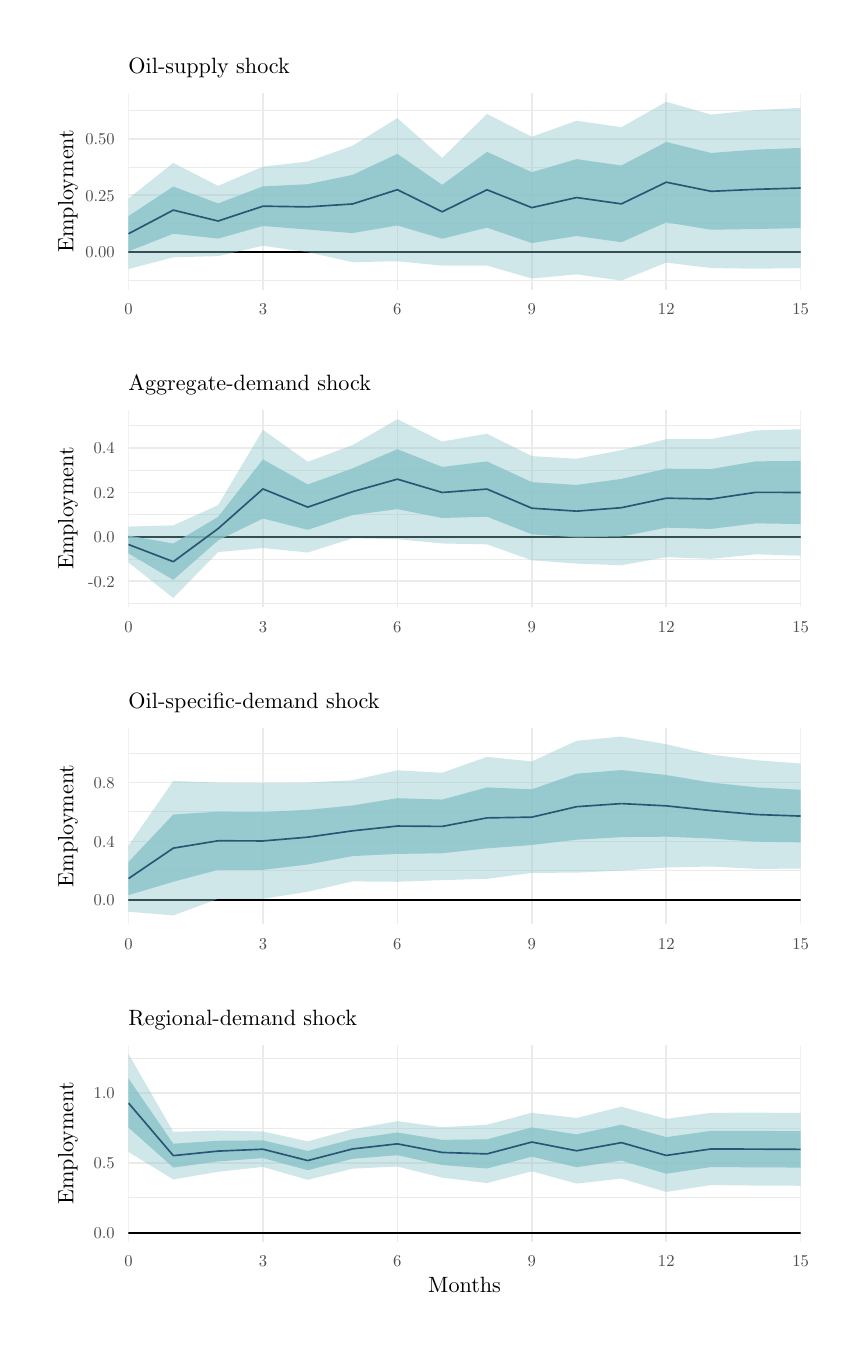
\begin{tikzpicture}[x=1pt,y=1pt]
\definecolor{fillColor}{RGB}{255,255,255}
\path[use as bounding box,fill=fillColor,fill opacity=0.00] (0,0) rectangle (290.32,469.75);
\begin{scope}
\path[clip] (  0.00,  0.00) rectangle (290.32,469.75);
\definecolor{drawColor}{RGB}{255,255,255}
\definecolor{fillColor}{RGB}{255,255,255}

\path[draw=drawColor,line width= 0.6pt,line join=round,line cap=round,fill=fillColor] (  0.00,  0.00) rectangle (290.32,469.76);
\end{scope}
\begin{scope}
\path[clip] (  5.50,349.57) rectangle (284.82,464.26);
\definecolor{fillColor}{RGB}{255,255,255}

\path[fill=fillColor] (  5.50,349.57) rectangle (284.82,464.26);
\end{scope}
\begin{scope}
\path[clip] (  5.50,234.88) rectangle (284.82,349.57);
\definecolor{fillColor}{RGB}{255,255,255}

\path[fill=fillColor] (  5.50,234.88) rectangle (284.82,349.57);
\end{scope}
\begin{scope}
\path[clip] (  5.50,120.19) rectangle (284.82,234.88);
\definecolor{fillColor}{RGB}{255,255,255}

\path[fill=fillColor] (  5.50,120.19) rectangle (284.82,234.88);
\end{scope}
\begin{scope}
\path[clip] (  5.50,  5.50) rectangle (284.82,120.19);
\definecolor{fillColor}{RGB}{255,255,255}

\path[fill=fillColor] (  5.50,  5.50) rectangle (284.82,120.19);
\end{scope}
\begin{scope}
\path[clip] ( 36.43,375.13) rectangle (279.32,446.19);
\definecolor{drawColor}{gray}{0.92}

\path[draw=drawColor,line width= 0.3pt,line join=round] ( 36.43,378.57) --
	(279.32,378.57);

\path[draw=drawColor,line width= 0.3pt,line join=round] ( 36.43,398.97) --
	(279.32,398.97);

\path[draw=drawColor,line width= 0.3pt,line join=round] ( 36.43,419.37) --
	(279.32,419.37);

\path[draw=drawColor,line width= 0.3pt,line join=round] ( 36.43,439.77) --
	(279.32,439.77);

\path[draw=drawColor,line width= 0.6pt,line join=round] ( 36.43,388.77) --
	(279.32,388.77);

\path[draw=drawColor,line width= 0.6pt,line join=round] ( 36.43,409.17) --
	(279.32,409.17);

\path[draw=drawColor,line width= 0.6pt,line join=round] ( 36.43,429.57) --
	(279.32,429.57);

\path[draw=drawColor,line width= 0.6pt,line join=round] ( 36.43,375.13) --
	( 36.43,446.19);

\path[draw=drawColor,line width= 0.6pt,line join=round] ( 85.01,375.13) --
	( 85.01,446.19);

\path[draw=drawColor,line width= 0.6pt,line join=round] (133.59,375.13) --
	(133.59,446.19);

\path[draw=drawColor,line width= 0.6pt,line join=round] (182.17,375.13) --
	(182.17,446.19);

\path[draw=drawColor,line width= 0.6pt,line join=round] (230.75,375.13) --
	(230.75,446.19);

\path[draw=drawColor,line width= 0.6pt,line join=round] (279.32,375.13) --
	(279.32,446.19);
\definecolor{drawColor}{RGB}{0,0,0}

\path[draw=drawColor,line width= 0.6pt,line join=round] ( 36.43,388.77) -- (279.32,388.77);
\definecolor{fillColor}{RGB}{136,195,200}

\path[fill=fillColor,fill opacity=0.40] ( 36.43,408.02) --
	( 52.62,420.86) --
	( 68.82,412.57) --
	( 85.01,419.53) --
	(101.20,421.36) --
	(117.39,427.06) --
	(133.59,437.05) --
	(149.78,422.67) --
	(165.97,438.55) --
	(182.17,430.32) --
	(198.36,436.12) --
	(214.55,433.78) --
	(230.75,442.96) --
	(246.94,438.33) --
	(263.13,440.01) --
	(279.32,440.77) --
	(279.32,382.84) --
	(263.13,382.65) --
	(246.94,382.88) --
	(230.75,384.87) --
	(214.55,378.36) --
	(198.36,380.60) --
	(182.17,379.12) --
	(165.97,383.80) --
	(149.78,383.76) --
	(133.59,385.34) --
	(117.39,385.01) --
	(101.20,388.62) --
	( 85.01,390.95) --
	( 68.82,387.20) --
	( 52.62,386.77) --
	( 36.43,382.54) --
	cycle;

\path[] ( 36.43,408.02) --
	( 52.62,420.86) --
	( 68.82,412.57) --
	( 85.01,419.53) --
	(101.20,421.36) --
	(117.39,427.06) --
	(133.59,437.05) --
	(149.78,422.67) --
	(165.97,438.55) --
	(182.17,430.32) --
	(198.36,436.12) --
	(214.55,433.78) --
	(230.75,442.96) --
	(246.94,438.33) --
	(263.13,440.01) --
	(279.32,440.77);

\path[] (279.32,382.84) --
	(263.13,382.65) --
	(246.94,382.88) --
	(230.75,384.87) --
	(214.55,378.36) --
	(198.36,380.60) --
	(182.17,379.12) --
	(165.97,383.80) --
	(149.78,383.76) --
	(133.59,385.34) --
	(117.39,385.01) --
	(101.20,388.62) --
	( 85.01,390.95) --
	( 68.82,387.20) --
	( 52.62,386.77) --
	( 36.43,382.54);
\definecolor{fillColor}{RGB}{136,195,200}

\path[fill=fillColor,fill opacity=0.80] ( 36.43,401.65) --
	( 52.62,412.34) --
	( 68.82,406.23) --
	( 85.01,412.39) --
	(101.20,413.18) --
	(117.39,416.55) --
	(133.59,424.12) --
	(149.78,412.94) --
	(165.97,424.86) --
	(182.17,417.52) --
	(198.36,422.24) --
	(214.55,419.93) --
	(230.75,428.44) --
	(246.94,424.47) --
	(263.13,425.67) --
	(279.32,426.29) --
	(279.32,397.32) --
	(263.13,396.99) --
	(246.94,396.74) --
	(230.75,399.39) --
	(214.55,392.22) --
	(198.36,394.48) --
	(182.17,391.92) --
	(165.97,397.48) --
	(149.78,393.49) --
	(133.59,398.27) --
	(117.39,395.52) --
	(101.20,396.80) --
	( 85.01,398.09) --
	( 68.82,393.54) --
	( 52.62,395.30) --
	( 36.43,388.91) --
	cycle;

\path[] ( 36.43,401.65) --
	( 52.62,412.34) --
	( 68.82,406.23) --
	( 85.01,412.39) --
	(101.20,413.18) --
	(117.39,416.55) --
	(133.59,424.12) --
	(149.78,412.94) --
	(165.97,424.86) --
	(182.17,417.52) --
	(198.36,422.24) --
	(214.55,419.93) --
	(230.75,428.44) --
	(246.94,424.47) --
	(263.13,425.67) --
	(279.32,426.29);

\path[] (279.32,397.32) --
	(263.13,396.99) --
	(246.94,396.74) --
	(230.75,399.39) --
	(214.55,392.22) --
	(198.36,394.48) --
	(182.17,391.92) --
	(165.97,397.48) --
	(149.78,393.49) --
	(133.59,398.27) --
	(117.39,395.52) --
	(101.20,396.80) --
	( 85.01,398.09) --
	( 68.82,393.54) --
	( 52.62,395.30) --
	( 36.43,388.91);
\definecolor{drawColor}{RGB}{42,86,118}

\path[draw=drawColor,line width= 0.6pt,line join=round] ( 36.43,395.28) --
	( 52.62,403.82) --
	( 68.82,399.88) --
	( 85.01,405.24) --
	(101.20,404.99) --
	(117.39,406.04) --
	(133.59,411.20) --
	(149.78,403.22) --
	(165.97,411.17) --
	(182.17,404.72) --
	(198.36,408.36) --
	(214.55,406.07) --
	(230.75,413.91) --
	(246.94,410.61) --
	(263.13,411.33) --
	(279.32,411.80);
\end{scope}
\begin{scope}
\path[clip] (  0.00,  0.00) rectangle (290.32,469.75);
\definecolor{drawColor}{gray}{0.30}

\node[text=drawColor,anchor=base east,inner sep=0pt, outer sep=0pt, scale=  0.60] at ( 31.48,386.70) {0.00};

\node[text=drawColor,anchor=base east,inner sep=0pt, outer sep=0pt, scale=  0.60] at ( 31.48,407.11) {0.25};

\node[text=drawColor,anchor=base east,inner sep=0pt, outer sep=0pt, scale=  0.60] at ( 31.48,427.51) {0.50};
\end{scope}
\begin{scope}
\path[clip] (  0.00,  0.00) rectangle (290.32,469.75);
\definecolor{drawColor}{gray}{0.30}

\node[text=drawColor,anchor=base,inner sep=0pt, outer sep=0pt, scale=  0.60] at ( 36.43,366.05) {0};

\node[text=drawColor,anchor=base,inner sep=0pt, outer sep=0pt, scale=  0.60] at ( 85.01,366.05) {3};

\node[text=drawColor,anchor=base,inner sep=0pt, outer sep=0pt, scale=  0.60] at (133.59,366.05) {6};

\node[text=drawColor,anchor=base,inner sep=0pt, outer sep=0pt, scale=  0.60] at (182.17,366.05) {9};

\node[text=drawColor,anchor=base,inner sep=0pt, outer sep=0pt, scale=  0.60] at (230.75,366.05) {12};

\node[text=drawColor,anchor=base,inner sep=0pt, outer sep=0pt, scale=  0.60] at (279.32,366.05) {15};
\end{scope}
\begin{scope}
\path[clip] (  0.00,  0.00) rectangle (290.32,469.75);
\definecolor{drawColor}{RGB}{0,0,0}

\node[text=drawColor,rotate= 90.00,anchor=base,inner sep=0pt, outer sep=0pt, scale=  0.80] at ( 16.51,410.66) {Employment};
\end{scope}
\begin{scope}
\path[clip] (  0.00,  0.00) rectangle (290.32,469.75);
\definecolor{drawColor}{RGB}{0,0,0}

\node[text=drawColor,anchor=base west,inner sep=0pt, outer sep=0pt, scale=  0.80] at ( 36.43,453.25) {Oil-supply shock};
\end{scope}
\begin{scope}
\path[clip] ( 36.43,260.44) rectangle (279.32,331.50);
\definecolor{drawColor}{gray}{0.92}

\path[draw=drawColor,line width= 0.3pt,line join=round] ( 36.43,261.67) --
	(279.32,261.67);

\path[draw=drawColor,line width= 0.3pt,line join=round] ( 36.43,277.71) --
	(279.32,277.71);

\path[draw=drawColor,line width= 0.3pt,line join=round] ( 36.43,293.76) --
	(279.32,293.76);

\path[draw=drawColor,line width= 0.3pt,line join=round] ( 36.43,309.80) --
	(279.32,309.80);

\path[draw=drawColor,line width= 0.3pt,line join=round] ( 36.43,325.85) --
	(279.32,325.85);

\path[draw=drawColor,line width= 0.6pt,line join=round] ( 36.43,269.69) --
	(279.32,269.69);

\path[draw=drawColor,line width= 0.6pt,line join=round] ( 36.43,285.74) --
	(279.32,285.74);

\path[draw=drawColor,line width= 0.6pt,line join=round] ( 36.43,301.78) --
	(279.32,301.78);

\path[draw=drawColor,line width= 0.6pt,line join=round] ( 36.43,317.82) --
	(279.32,317.82);

\path[draw=drawColor,line width= 0.6pt,line join=round] ( 36.43,260.44) --
	( 36.43,331.50);

\path[draw=drawColor,line width= 0.6pt,line join=round] ( 85.01,260.44) --
	( 85.01,331.50);

\path[draw=drawColor,line width= 0.6pt,line join=round] (133.59,260.44) --
	(133.59,331.50);

\path[draw=drawColor,line width= 0.6pt,line join=round] (182.17,260.44) --
	(182.17,331.50);

\path[draw=drawColor,line width= 0.6pt,line join=round] (230.75,260.44) --
	(230.75,331.50);

\path[draw=drawColor,line width= 0.6pt,line join=round] (279.32,260.44) --
	(279.32,331.50);
\definecolor{drawColor}{RGB}{0,0,0}

\path[draw=drawColor,line width= 0.6pt,line join=round] ( 36.43,285.74) -- (279.32,285.74);
\definecolor{fillColor}{RGB}{136,195,200}

\path[fill=fillColor,fill opacity=0.40] ( 36.43,289.47) --
	( 52.62,289.90) --
	( 68.82,297.21) --
	( 85.01,324.43) --
	(101.20,312.88) --
	(117.39,318.91) --
	(133.59,328.27) --
	(149.78,320.22) --
	(165.97,323.00) --
	(182.17,314.93) --
	(198.36,313.98) --
	(214.55,317.09) --
	(230.75,321.03) --
	(246.94,321.07) --
	(263.13,324.23) --
	(279.32,324.62) --
	(279.32,278.96) --
	(263.13,279.45) --
	(246.94,277.80) --
	(230.75,278.42) --
	(214.55,275.49) --
	(198.36,276.09) --
	(182.17,277.29) --
	(165.97,283.05) --
	(149.78,283.36) --
	(133.59,284.93) --
	(117.39,285.23) --
	(101.20,280.10) --
	( 85.01,281.71) --
	( 68.82,280.25) --
	( 52.62,263.67) --
	( 36.43,276.51) --
	cycle;

\path[] ( 36.43,289.47) --
	( 52.62,289.90) --
	( 68.82,297.21) --
	( 85.01,324.43) --
	(101.20,312.88) --
	(117.39,318.91) --
	(133.59,328.27) --
	(149.78,320.22) --
	(165.97,323.00) --
	(182.17,314.93) --
	(198.36,313.98) --
	(214.55,317.09) --
	(230.75,321.03) --
	(246.94,321.07) --
	(263.13,324.23) --
	(279.32,324.62);

\path[] (279.32,278.96) --
	(263.13,279.45) --
	(246.94,277.80) --
	(230.75,278.42) --
	(214.55,275.49) --
	(198.36,276.09) --
	(182.17,277.29) --
	(165.97,283.05) --
	(149.78,283.36) --
	(133.59,284.93) --
	(117.39,285.23) --
	(101.20,280.10) --
	( 85.01,281.71) --
	( 68.82,280.25) --
	( 52.62,263.67) --
	( 36.43,276.51);
\definecolor{fillColor}{RGB}{136,195,200}

\path[fill=fillColor,fill opacity=0.80] ( 36.43,286.23) --
	( 52.62,283.34) --
	( 68.82,292.97) --
	( 85.01,313.75) --
	(101.20,304.68) --
	(117.39,310.49) --
	(133.59,317.44) --
	(149.78,311.01) --
	(165.97,313.01) --
	(182.17,305.52) --
	(198.36,304.51) --
	(214.55,306.69) --
	(230.75,310.38) --
	(246.94,310.25) --
	(263.13,313.03) --
	(279.32,313.21) --
	(279.32,290.37) --
	(263.13,290.64) --
	(246.94,288.62) --
	(230.75,289.07) --
	(214.55,285.89) --
	(198.36,285.56) --
	(182.17,286.70) --
	(165.97,293.03) --
	(149.78,292.58) --
	(133.59,295.77) --
	(117.39,293.65) --
	(101.20,288.30) --
	( 85.01,292.39) --
	( 68.82,284.49) --
	( 52.62,270.23) --
	( 36.43,279.75) --
	cycle;

\path[] ( 36.43,286.23) --
	( 52.62,283.34) --
	( 68.82,292.97) --
	( 85.01,313.75) --
	(101.20,304.68) --
	(117.39,310.49) --
	(133.59,317.44) --
	(149.78,311.01) --
	(165.97,313.01) --
	(182.17,305.52) --
	(198.36,304.51) --
	(214.55,306.69) --
	(230.75,310.38) --
	(246.94,310.25) --
	(263.13,313.03) --
	(279.32,313.21);

\path[] (279.32,290.37) --
	(263.13,290.64) --
	(246.94,288.62) --
	(230.75,289.07) --
	(214.55,285.89) --
	(198.36,285.56) --
	(182.17,286.70) --
	(165.97,293.03) --
	(149.78,292.58) --
	(133.59,295.77) --
	(117.39,293.65) --
	(101.20,288.30) --
	( 85.01,292.39) --
	( 68.82,284.49) --
	( 52.62,270.23) --
	( 36.43,279.75);
\definecolor{drawColor}{RGB}{42,86,118}

\path[draw=drawColor,line width= 0.6pt,line join=round] ( 36.43,282.99) --
	( 52.62,276.78) --
	( 68.82,288.73) --
	( 85.01,303.07) --
	(101.20,296.49) --
	(117.39,302.07) --
	(133.59,306.60) --
	(149.78,301.79) --
	(165.97,303.02) --
	(182.17,296.11) --
	(198.36,295.04) --
	(214.55,296.29) --
	(230.75,299.72) --
	(246.94,299.43) --
	(263.13,301.84) --
	(279.32,301.79);
\end{scope}
\begin{scope}
\path[clip] (  0.00,  0.00) rectangle (290.32,469.75);
\definecolor{drawColor}{gray}{0.30}

\node[text=drawColor,anchor=base east,inner sep=0pt, outer sep=0pt, scale=  0.60] at ( 31.48,267.63) {-0.2};

\node[text=drawColor,anchor=base east,inner sep=0pt, outer sep=0pt, scale=  0.60] at ( 31.48,283.67) {0.0};

\node[text=drawColor,anchor=base east,inner sep=0pt, outer sep=0pt, scale=  0.60] at ( 31.48,299.71) {0.2};

\node[text=drawColor,anchor=base east,inner sep=0pt, outer sep=0pt, scale=  0.60] at ( 31.48,315.76) {0.4};
\end{scope}
\begin{scope}
\path[clip] (  0.00,  0.00) rectangle (290.32,469.75);
\definecolor{drawColor}{gray}{0.30}

\node[text=drawColor,anchor=base,inner sep=0pt, outer sep=0pt, scale=  0.60] at ( 36.43,251.36) {0};

\node[text=drawColor,anchor=base,inner sep=0pt, outer sep=0pt, scale=  0.60] at ( 85.01,251.36) {3};

\node[text=drawColor,anchor=base,inner sep=0pt, outer sep=0pt, scale=  0.60] at (133.59,251.36) {6};

\node[text=drawColor,anchor=base,inner sep=0pt, outer sep=0pt, scale=  0.60] at (182.17,251.36) {9};

\node[text=drawColor,anchor=base,inner sep=0pt, outer sep=0pt, scale=  0.60] at (230.75,251.36) {12};

\node[text=drawColor,anchor=base,inner sep=0pt, outer sep=0pt, scale=  0.60] at (279.32,251.36) {15};
\end{scope}
\begin{scope}
\path[clip] (  0.00,  0.00) rectangle (290.32,469.75);
\definecolor{drawColor}{RGB}{0,0,0}

\node[text=drawColor,rotate= 90.00,anchor=base,inner sep=0pt, outer sep=0pt, scale=  0.80] at ( 16.51,295.97) {Employment};
\end{scope}
\begin{scope}
\path[clip] (  0.00,  0.00) rectangle (290.32,469.75);
\definecolor{drawColor}{RGB}{0,0,0}

\node[text=drawColor,anchor=base west,inner sep=0pt, outer sep=0pt, scale=  0.80] at ( 36.43,338.56) {Aggregate-demand shock};
\end{scope}
\begin{scope}
\path[clip] ( 36.43,145.75) rectangle (279.32,216.81);
\definecolor{drawColor}{gray}{0.92}

\path[draw=drawColor,line width= 0.3pt,line join=round] ( 36.43,165.09) --
	(279.32,165.09);

\path[draw=drawColor,line width= 0.3pt,line join=round] ( 36.43,186.38) --
	(279.32,186.38);

\path[draw=drawColor,line width= 0.3pt,line join=round] ( 36.43,207.67) --
	(279.32,207.67);

\path[draw=drawColor,line width= 0.6pt,line join=round] ( 36.43,154.44) --
	(279.32,154.44);

\path[draw=drawColor,line width= 0.6pt,line join=round] ( 36.43,175.73) --
	(279.32,175.73);

\path[draw=drawColor,line width= 0.6pt,line join=round] ( 36.43,197.03) --
	(279.32,197.03);

\path[draw=drawColor,line width= 0.6pt,line join=round] ( 36.43,145.75) --
	( 36.43,216.81);

\path[draw=drawColor,line width= 0.6pt,line join=round] ( 85.01,145.75) --
	( 85.01,216.81);

\path[draw=drawColor,line width= 0.6pt,line join=round] (133.59,145.75) --
	(133.59,216.81);

\path[draw=drawColor,line width= 0.6pt,line join=round] (182.17,145.75) --
	(182.17,216.81);

\path[draw=drawColor,line width= 0.6pt,line join=round] (230.75,145.75) --
	(230.75,216.81);

\path[draw=drawColor,line width= 0.6pt,line join=round] (279.32,145.75) --
	(279.32,216.81);
\definecolor{drawColor}{RGB}{0,0,0}

\path[draw=drawColor,line width= 0.6pt,line join=round] ( 36.43,154.44) -- (279.32,154.44);
\definecolor{fillColor}{RGB}{136,195,200}

\path[fill=fillColor,fill opacity=0.40] ( 36.43,174.25) --
	( 52.62,197.56) --
	( 68.82,196.95) --
	( 85.01,196.81) --
	(101.20,196.97) --
	(117.39,197.82) --
	(133.59,201.39) --
	(149.78,200.52) --
	(165.97,206.24) --
	(182.17,204.60) --
	(198.36,212.07) --
	(214.55,213.58) --
	(230.75,210.82) --
	(246.94,207.06) --
	(263.13,205.06) --
	(279.32,203.86) --
	(279.32,165.87) --
	(263.13,165.78) --
	(246.94,166.64) --
	(230.75,166.27) --
	(214.55,165.16) --
	(198.36,164.42) --
	(182.17,164.33) --
	(165.97,162.18) --
	(149.78,161.72) --
	(133.59,161.12) --
	(117.39,161.25) --
	(101.20,157.52) --
	( 85.01,154.94) --
	( 68.82,154.92) --
	( 52.62,148.98) --
	( 36.43,150.29) --
	cycle;

\path[] ( 36.43,174.25) --
	( 52.62,197.56) --
	( 68.82,196.95) --
	( 85.01,196.81) --
	(101.20,196.97) --
	(117.39,197.82) --
	(133.59,201.39) --
	(149.78,200.52) --
	(165.97,206.24) --
	(182.17,204.60) --
	(198.36,212.07) --
	(214.55,213.58) --
	(230.75,210.82) --
	(246.94,207.06) --
	(263.13,205.06) --
	(279.32,203.86);

\path[] (279.32,165.87) --
	(263.13,165.78) --
	(246.94,166.64) --
	(230.75,166.27) --
	(214.55,165.16) --
	(198.36,164.42) --
	(182.17,164.33) --
	(165.97,162.18) --
	(149.78,161.72) --
	(133.59,161.12) --
	(117.39,161.25) --
	(101.20,157.52) --
	( 85.01,154.94) --
	( 68.82,154.92) --
	( 52.62,148.98) --
	( 36.43,150.29);
\definecolor{fillColor}{RGB}{136,195,200}

\path[fill=fillColor,fill opacity=0.80] ( 36.43,168.26) --
	( 52.62,185.42) --
	( 68.82,186.45) --
	( 85.01,186.34) --
	(101.20,187.10) --
	(117.39,188.68) --
	(133.59,191.32) --
	(149.78,190.82) --
	(165.97,195.22) --
	(182.17,194.53) --
	(198.36,200.16) --
	(214.55,201.48) --
	(230.75,199.68) --
	(246.94,196.96) --
	(263.13,195.24) --
	(279.32,194.36) --
	(279.32,175.37) --
	(263.13,175.60) --
	(246.94,176.75) --
	(230.75,177.41) --
	(214.55,177.26) --
	(198.36,176.33) --
	(182.17,174.40) --
	(165.97,173.20) --
	(149.78,171.42) --
	(133.59,171.19) --
	(117.39,170.39) --
	(101.20,167.38) --
	( 85.01,165.41) --
	( 68.82,165.43) --
	( 52.62,161.13) --
	( 36.43,156.28) --
	cycle;

\path[] ( 36.43,168.26) --
	( 52.62,185.42) --
	( 68.82,186.45) --
	( 85.01,186.34) --
	(101.20,187.10) --
	(117.39,188.68) --
	(133.59,191.32) --
	(149.78,190.82) --
	(165.97,195.22) --
	(182.17,194.53) --
	(198.36,200.16) --
	(214.55,201.48) --
	(230.75,199.68) --
	(246.94,196.96) --
	(263.13,195.24) --
	(279.32,194.36);

\path[] (279.32,175.37) --
	(263.13,175.60) --
	(246.94,176.75) --
	(230.75,177.41) --
	(214.55,177.26) --
	(198.36,176.33) --
	(182.17,174.40) --
	(165.97,173.20) --
	(149.78,171.42) --
	(133.59,171.19) --
	(117.39,170.39) --
	(101.20,167.38) --
	( 85.01,165.41) --
	( 68.82,165.43) --
	( 52.62,161.13) --
	( 36.43,156.28);
\definecolor{drawColor}{RGB}{42,86,118}

\path[draw=drawColor,line width= 0.6pt,line join=round] ( 36.43,162.27) --
	( 52.62,173.27) --
	( 68.82,175.94) --
	( 85.01,175.87) --
	(101.20,177.24) --
	(117.39,179.53) --
	(133.59,181.25) --
	(149.78,181.12) --
	(165.97,184.21) --
	(182.17,184.47) --
	(198.36,188.25) --
	(214.55,189.37) --
	(230.75,188.55) --
	(246.94,186.85) --
	(263.13,185.42) --
	(279.32,184.86);
\end{scope}
\begin{scope}
\path[clip] (  0.00,  0.00) rectangle (290.32,469.75);
\definecolor{drawColor}{gray}{0.30}

\node[text=drawColor,anchor=base east,inner sep=0pt, outer sep=0pt, scale=  0.60] at ( 31.48,152.37) {0.0};

\node[text=drawColor,anchor=base east,inner sep=0pt, outer sep=0pt, scale=  0.60] at ( 31.48,173.67) {0.4};

\node[text=drawColor,anchor=base east,inner sep=0pt, outer sep=0pt, scale=  0.60] at ( 31.48,194.96) {0.8};
\end{scope}
\begin{scope}
\path[clip] (  0.00,  0.00) rectangle (290.32,469.75);
\definecolor{drawColor}{gray}{0.30}

\node[text=drawColor,anchor=base,inner sep=0pt, outer sep=0pt, scale=  0.60] at ( 36.43,136.67) {0};

\node[text=drawColor,anchor=base,inner sep=0pt, outer sep=0pt, scale=  0.60] at ( 85.01,136.67) {3};

\node[text=drawColor,anchor=base,inner sep=0pt, outer sep=0pt, scale=  0.60] at (133.59,136.67) {6};

\node[text=drawColor,anchor=base,inner sep=0pt, outer sep=0pt, scale=  0.60] at (182.17,136.67) {9};

\node[text=drawColor,anchor=base,inner sep=0pt, outer sep=0pt, scale=  0.60] at (230.75,136.67) {12};

\node[text=drawColor,anchor=base,inner sep=0pt, outer sep=0pt, scale=  0.60] at (279.32,136.67) {15};
\end{scope}
\begin{scope}
\path[clip] (  0.00,  0.00) rectangle (290.32,469.75);
\definecolor{drawColor}{RGB}{0,0,0}

\node[text=drawColor,rotate= 90.00,anchor=base,inner sep=0pt, outer sep=0pt, scale=  0.80] at ( 16.51,181.28) {Employment};
\end{scope}
\begin{scope}
\path[clip] (  0.00,  0.00) rectangle (290.32,469.75);
\definecolor{drawColor}{RGB}{0,0,0}

\node[text=drawColor,anchor=base west,inner sep=0pt, outer sep=0pt, scale=  0.80] at ( 36.43,223.87) {Oil-specific-demand shock};
\end{scope}
\begin{scope}
\path[clip] ( 36.43, 31.06) rectangle (279.32,102.12);
\definecolor{drawColor}{gray}{0.92}

\path[draw=drawColor,line width= 0.3pt,line join=round] ( 36.43, 46.91) --
	(279.32, 46.91);

\path[draw=drawColor,line width= 0.3pt,line join=round] ( 36.43, 72.13) --
	(279.32, 72.13);

\path[draw=drawColor,line width= 0.3pt,line join=round] ( 36.43, 97.36) --
	(279.32, 97.36);

\path[draw=drawColor,line width= 0.6pt,line join=round] ( 36.43, 34.29) --
	(279.32, 34.29);

\path[draw=drawColor,line width= 0.6pt,line join=round] ( 36.43, 59.52) --
	(279.32, 59.52);

\path[draw=drawColor,line width= 0.6pt,line join=round] ( 36.43, 84.74) --
	(279.32, 84.74);

\path[draw=drawColor,line width= 0.6pt,line join=round] ( 36.43, 31.06) --
	( 36.43,102.12);

\path[draw=drawColor,line width= 0.6pt,line join=round] ( 85.01, 31.06) --
	( 85.01,102.12);

\path[draw=drawColor,line width= 0.6pt,line join=round] (133.59, 31.06) --
	(133.59,102.12);

\path[draw=drawColor,line width= 0.6pt,line join=round] (182.17, 31.06) --
	(182.17,102.12);

\path[draw=drawColor,line width= 0.6pt,line join=round] (230.75, 31.06) --
	(230.75,102.12);

\path[draw=drawColor,line width= 0.6pt,line join=round] (279.32, 31.06) --
	(279.32,102.12);
\definecolor{drawColor}{RGB}{0,0,0}

\path[draw=drawColor,line width= 0.6pt,line join=round] ( 36.43, 34.29) -- (279.32, 34.29);
\definecolor{fillColor}{RGB}{136,195,200}

\path[fill=fillColor,fill opacity=0.40] ( 36.43, 98.89) --
	( 52.62, 70.76) --
	( 68.82, 71.26) --
	( 85.01, 70.88) --
	(101.20, 67.32) --
	(117.39, 71.71) --
	(133.59, 74.62) --
	(149.78, 72.41) --
	(165.97, 73.33) --
	(182.17, 77.64) --
	(198.36, 75.76) --
	(214.55, 79.84) --
	(230.75, 75.43) --
	(246.94, 77.64) --
	(263.13, 77.68) --
	(279.32, 77.60) --
	(279.32, 51.27) --
	(263.13, 51.34) --
	(246.94, 51.52) --
	(230.75, 49.03) --
	(214.55, 53.88) --
	(198.36, 52.07) --
	(182.17, 56.50) --
	(165.97, 52.25) --
	(149.78, 54.21) --
	(133.59, 58.22) --
	(117.39, 57.46) --
	(101.20, 53.43) --
	( 85.01, 58.08) --
	( 68.82, 56.33) --
	( 52.62, 53.56) --
	( 36.43, 63.46) --
	cycle;

\path[] ( 36.43, 98.89) --
	( 52.62, 70.76) --
	( 68.82, 71.26) --
	( 85.01, 70.88) --
	(101.20, 67.32) --
	(117.39, 71.71) --
	(133.59, 74.62) --
	(149.78, 72.41) --
	(165.97, 73.33) --
	(182.17, 77.64) --
	(198.36, 75.76) --
	(214.55, 79.84) --
	(230.75, 75.43) --
	(246.94, 77.64) --
	(263.13, 77.68) --
	(279.32, 77.60);

\path[] (279.32, 51.27) --
	(263.13, 51.34) --
	(246.94, 51.52) --
	(230.75, 49.03) --
	(214.55, 53.88) --
	(198.36, 52.07) --
	(182.17, 56.50) --
	(165.97, 52.25) --
	(149.78, 54.21) --
	(133.59, 58.22) --
	(117.39, 57.46) --
	(101.20, 53.43) --
	( 85.01, 58.08) --
	( 68.82, 56.33) --
	( 52.62, 53.56) --
	( 36.43, 63.46);
\definecolor{fillColor}{RGB}{136,195,200}

\path[fill=fillColor,fill opacity=0.80] ( 36.43, 90.04) --
	( 52.62, 66.46) --
	( 68.82, 67.53) --
	( 85.01, 67.68) --
	(101.20, 63.85) --
	(117.39, 68.15) --
	(133.59, 70.52) --
	(149.78, 67.86) --
	(165.97, 68.06) --
	(182.17, 72.35) --
	(198.36, 69.84) --
	(214.55, 73.35) --
	(230.75, 68.83) --
	(246.94, 71.11) --
	(263.13, 71.09) --
	(279.32, 71.02) --
	(279.32, 57.85) --
	(263.13, 57.92) --
	(246.94, 58.05) --
	(230.75, 55.63) --
	(214.55, 60.37) --
	(198.36, 57.99) --
	(182.17, 61.79) --
	(165.97, 57.52) --
	(149.78, 58.76) --
	(133.59, 62.32) --
	(117.39, 61.02) --
	(101.20, 56.91) --
	( 85.01, 61.28) --
	( 68.82, 60.06) --
	( 52.62, 57.86) --
	( 36.43, 72.32) --
	cycle;

\path[] ( 36.43, 90.04) --
	( 52.62, 66.46) --
	( 68.82, 67.53) --
	( 85.01, 67.68) --
	(101.20, 63.85) --
	(117.39, 68.15) --
	(133.59, 70.52) --
	(149.78, 67.86) --
	(165.97, 68.06) --
	(182.17, 72.35) --
	(198.36, 69.84) --
	(214.55, 73.35) --
	(230.75, 68.83) --
	(246.94, 71.11) --
	(263.13, 71.09) --
	(279.32, 71.02);

\path[] (279.32, 57.85) --
	(263.13, 57.92) --
	(246.94, 58.05) --
	(230.75, 55.63) --
	(214.55, 60.37) --
	(198.36, 57.99) --
	(182.17, 61.79) --
	(165.97, 57.52) --
	(149.78, 58.76) --
	(133.59, 62.32) --
	(117.39, 61.02) --
	(101.20, 56.91) --
	( 85.01, 61.28) --
	( 68.82, 60.06) --
	( 52.62, 57.86) --
	( 36.43, 72.32);
\definecolor{drawColor}{RGB}{42,86,118}

\path[draw=drawColor,line width= 0.6pt,line join=round] ( 36.43, 81.18) --
	( 52.62, 62.16) --
	( 68.82, 63.80) --
	( 85.01, 64.48) --
	(101.20, 60.38) --
	(117.39, 64.58) --
	(133.59, 66.42) --
	(149.78, 63.31) --
	(165.97, 62.79) --
	(182.17, 67.07) --
	(198.36, 63.92) --
	(214.55, 66.86) --
	(230.75, 62.23) --
	(246.94, 64.58) --
	(263.13, 64.51) --
	(279.32, 64.43);
\end{scope}
\begin{scope}
\path[clip] (  0.00,  0.00) rectangle (290.32,469.75);
\definecolor{drawColor}{gray}{0.30}

\node[text=drawColor,anchor=base east,inner sep=0pt, outer sep=0pt, scale=  0.60] at ( 31.48, 32.23) {0.0};

\node[text=drawColor,anchor=base east,inner sep=0pt, outer sep=0pt, scale=  0.60] at ( 31.48, 57.45) {0.5};

\node[text=drawColor,anchor=base east,inner sep=0pt, outer sep=0pt, scale=  0.60] at ( 31.48, 82.68) {1.0};
\end{scope}
\begin{scope}
\path[clip] (  0.00,  0.00) rectangle (290.32,469.75);
\definecolor{drawColor}{gray}{0.30}

\node[text=drawColor,anchor=base,inner sep=0pt, outer sep=0pt, scale=  0.60] at ( 36.43, 21.98) {0};

\node[text=drawColor,anchor=base,inner sep=0pt, outer sep=0pt, scale=  0.60] at ( 85.01, 21.98) {3};

\node[text=drawColor,anchor=base,inner sep=0pt, outer sep=0pt, scale=  0.60] at (133.59, 21.98) {6};

\node[text=drawColor,anchor=base,inner sep=0pt, outer sep=0pt, scale=  0.60] at (182.17, 21.98) {9};

\node[text=drawColor,anchor=base,inner sep=0pt, outer sep=0pt, scale=  0.60] at (230.75, 21.98) {12};

\node[text=drawColor,anchor=base,inner sep=0pt, outer sep=0pt, scale=  0.60] at (279.32, 21.98) {15};
\end{scope}
\begin{scope}
\path[clip] (  0.00,  0.00) rectangle (290.32,469.75);
\definecolor{drawColor}{RGB}{0,0,0}

\node[text=drawColor,anchor=base,inner sep=0pt, outer sep=0pt, scale=  0.80] at (157.88, 12.56) {Months};
\end{scope}
\begin{scope}
\path[clip] (  0.00,  0.00) rectangle (290.32,469.75);
\definecolor{drawColor}{RGB}{0,0,0}

\node[text=drawColor,rotate= 90.00,anchor=base,inner sep=0pt, outer sep=0pt, scale=  0.80] at ( 16.51, 66.59) {Employment};
\end{scope}
\begin{scope}
\path[clip] (  0.00,  0.00) rectangle (290.32,469.75);
\definecolor{drawColor}{RGB}{0,0,0}

\node[text=drawColor,anchor=base west,inner sep=0pt, outer sep=0pt, scale=  0.80] at ( 36.43,109.18) {Regional-demand shock};
\end{scope}
\end{tikzpicture}
}
\caption{Cumulative employment responses to one-standard-deviation structural shocks in Kern County, California}
\end{figure}

\begin{figure}[htbp]
  \centering
  % \resizebox{<horizontal size>}{<vertical size>}{%
  \resizebox{0.8\textwidth}{!}{
  % Created by tikzDevice version 0.12.6 on 2026-02-22 21:44:02
% !TEX encoding = UTF-8 Unicode
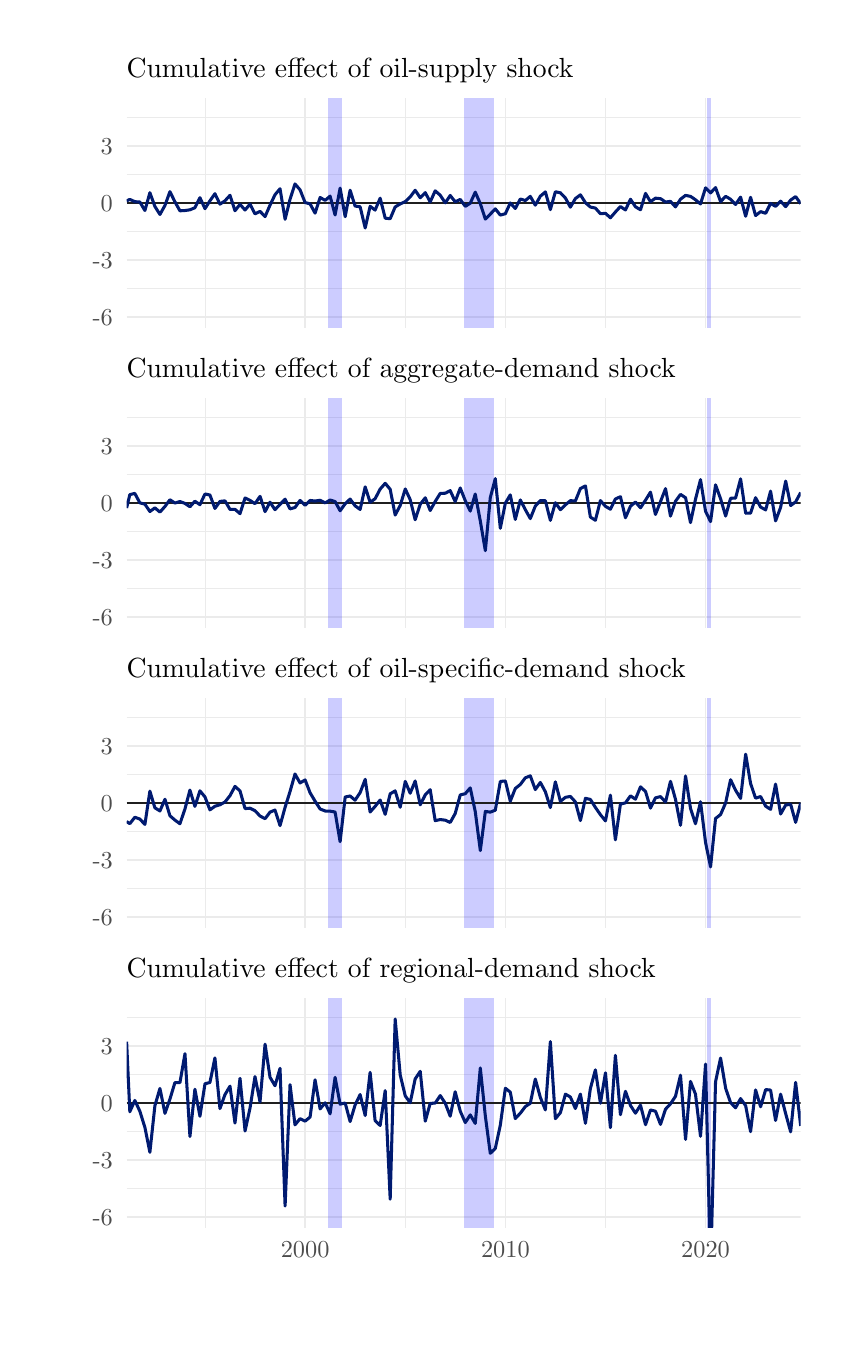
\begin{tikzpicture}[x=1pt,y=1pt]
\definecolor{fillColor}{RGB}{255,255,255}
\path[use as bounding box,fill=fillColor,fill opacity=0.00] (0,0) rectangle (290.32,469.75);
\begin{scope}
\path[clip] ( 35.75,361.36) rectangle (279.32,444.42);
\definecolor{drawColor}{gray}{0.92}

\path[draw=drawColor,line width= 0.3pt,line join=round] ( 35.75,375.44) --
	(279.32,375.44);

\path[draw=drawColor,line width= 0.3pt,line join=round] ( 35.75,396.03) --
	(279.32,396.03);

\path[draw=drawColor,line width= 0.3pt,line join=round] ( 35.75,416.62) --
	(279.32,416.62);

\path[draw=drawColor,line width= 0.3pt,line join=round] ( 35.75,437.22) --
	(279.32,437.22);

\path[draw=drawColor,line width= 0.3pt,line join=round] ( 64.07,361.36) --
	( 64.07,444.42);

\path[draw=drawColor,line width= 0.3pt,line join=round] (136.43,361.36) --
	(136.43,444.42);

\path[draw=drawColor,line width= 0.3pt,line join=round] (208.78,361.36) --
	(208.78,444.42);

\path[draw=drawColor,line width= 0.6pt,line join=round] ( 35.75,365.14) --
	(279.32,365.14);

\path[draw=drawColor,line width= 0.6pt,line join=round] ( 35.75,385.73) --
	(279.32,385.73);

\path[draw=drawColor,line width= 0.6pt,line join=round] ( 35.75,406.33) --
	(279.32,406.33);

\path[draw=drawColor,line width= 0.6pt,line join=round] ( 35.75,426.92) --
	(279.32,426.92);

\path[draw=drawColor,line width= 0.6pt,line join=round] (100.25,361.36) --
	(100.25,444.42);

\path[draw=drawColor,line width= 0.6pt,line join=round] (172.61,361.36) --
	(172.61,444.42);

\path[draw=drawColor,line width= 0.6pt,line join=round] (244.95,361.36) --
	(244.95,444.42);
\definecolor{fillColor}{RGB}{0,0,255}

\path[fill=fillColor,fill opacity=0.20] (108.66,361.36) rectangle (113.52,444.42);

\path[fill=fillColor,fill opacity=0.20] (157.52,361.36) rectangle (168.37,444.42);

\path[fill=fillColor,fill opacity=0.20] (245.57,361.36) rectangle (246.76,444.42);
\definecolor{drawColor}{gray}{0.12}

\path[draw=drawColor,line width= 0.6pt,line join=round] ( 35.75,406.33) -- (279.32,406.33);
\definecolor{drawColor}{RGB}{0,26,112}

\path[draw=drawColor,line width= 1.1pt,line join=round] ( 35.75,407.13) --
	( 36.91,407.69) --
	( 38.72,406.87) --
	( 40.54,406.75) --
	( 42.36,403.67) --
	( 44.16,410.11) --
	( 45.97,405.14) --
	( 47.79,402.25) --
	( 49.61,405.51) --
	( 51.40,410.49) --
	( 53.20,406.84) --
	( 55.02,403.57) --
	( 56.84,403.67) --
	( 58.63,403.93) --
	( 60.43,404.67) --
	( 62.25,408.31) --
	( 64.07,404.34) --
	( 65.86,407.18) --
	( 67.66,409.75) --
	( 69.48,405.97) --
	( 71.30,407.20) --
	( 73.11,409.17) --
	( 74.91,403.60) --
	( 76.73,405.89) --
	( 78.55,403.85) --
	( 80.34,405.99) --
	( 82.14,402.45) --
	( 83.96,403.38) --
	( 85.78,401.47) --
	( 87.57,405.62) --
	( 89.37,409.37) --
	( 91.19,411.54) --
	( 93.02,400.50) --
	( 94.80,407.73) --
	( 96.60,413.28) --
	( 98.42,411.15) --
	(100.25,406.56) --
	(102.05,406.07) --
	(103.85,402.72) --
	(105.67,408.38) --
	(107.50,407.34) --
	(109.28,408.88) --
	(111.08,402.06) --
	(112.90,411.77) --
	(114.73,401.43) --
	(116.51,411.02) --
	(118.31,405.28) --
	(120.13,405.03) --
	(121.96,397.36) --
	(123.74,405.21) --
	(125.54,403.83) --
	(127.37,408.13) --
	(129.19,400.90) --
	(130.99,400.71) --
	(132.79,404.96) --
	(134.62,406.06) --
	(136.44,406.89) --
	(138.22,408.60) --
	(140.02,410.99) --
	(141.85,408.29) --
	(143.67,410.14) --
	(145.45,406.76) --
	(147.25,410.79) --
	(149.08,409.19) --
	(150.90,406.45) --
	(152.68,409.11) --
	(154.48,406.82) --
	(156.31,407.68) --
	(158.13,405.18) --
	(159.93,406.32) --
	(161.73,410.32) --
	(163.56,406.15) --
	(165.38,400.58) --
	(167.16,402.36) --
	(168.97,404.28) --
	(170.79,402.02) --
	(172.61,402.51) --
	(174.39,406.41) --
	(176.20,404.41) --
	(178.02,407.84) --
	(179.84,407.28) --
	(181.62,408.79) --
	(183.43,405.61) --
	(185.25,408.85) --
	(187.07,410.39) --
	(188.87,404.00) --
	(190.68,410.45) --
	(192.50,410.08) --
	(194.32,408.17) --
	(196.10,404.87) --
	(197.91,407.99) --
	(199.73,409.34) --
	(201.55,406.49) --
	(203.33,404.94) --
	(205.14,404.55) --
	(206.96,402.52) --
	(208.78,402.65) --
	(210.57,401.05) --
	(212.37,403.13) --
	(214.19,405.12) --
	(216.01,403.88) --
	(217.82,407.76) --
	(219.62,405.03) --
	(221.44,403.94) --
	(223.26,409.85) --
	(225.05,406.86) --
	(226.85,408.14) --
	(228.67,407.96) --
	(230.49,406.74) --
	(232.28,406.98) --
	(234.08,404.98) --
	(235.90,407.76) --
	(237.72,409.15) --
	(239.51,408.79) --
	(241.31,407.56) --
	(243.13,406.04) --
	(244.95,411.87) --
	(246.76,410.04) --
	(248.56,411.95) --
	(250.38,406.89) --
	(252.21,408.80) --
	(253.99,407.75) --
	(255.79,405.86) --
	(257.61,408.51) --
	(259.44,401.59) --
	(261.22,408.45) --
	(263.02,401.85) --
	(264.84,403.27) --
	(266.67,402.67) --
	(268.45,406.23) --
	(270.25,405.18) --
	(272.07,407.05) --
	(273.90,405.06) --
	(275.70,407.47) --
	(277.50,408.70) --
	(279.32,406.16);
\end{scope}
\begin{scope}
\path[clip] (  0.00,  0.00) rectangle (290.32,469.75);
\definecolor{drawColor}{gray}{0.30}

\node[text=drawColor,anchor=base east,inner sep=0pt, outer sep=0pt, scale=  0.88] at ( 30.80,362.11) {-6};

\node[text=drawColor,anchor=base east,inner sep=0pt, outer sep=0pt, scale=  0.88] at ( 30.80,382.70) {-3};

\node[text=drawColor,anchor=base east,inner sep=0pt, outer sep=0pt, scale=  0.88] at ( 30.80,403.30) {0};

\node[text=drawColor,anchor=base east,inner sep=0pt, outer sep=0pt, scale=  0.88] at ( 30.80,423.89) {3};
\end{scope}
\begin{scope}
\path[clip] (  0.00,  0.00) rectangle (290.32,469.75);
\definecolor{drawColor}{RGB}{0,0,0}

\node[text=drawColor,anchor=base west,inner sep=0pt, outer sep=0pt, scale=  1.00] at ( 35.75,451.87) {Cumulative effect of oil-supply shock};
\end{scope}
\begin{scope}
\path[clip] ( 35.75,252.97) rectangle (279.32,336.03);
\definecolor{drawColor}{gray}{0.92}

\path[draw=drawColor,line width= 0.3pt,line join=round] ( 35.75,267.04) --
	(279.32,267.04);

\path[draw=drawColor,line width= 0.3pt,line join=round] ( 35.75,287.64) --
	(279.32,287.64);

\path[draw=drawColor,line width= 0.3pt,line join=round] ( 35.75,308.23) --
	(279.32,308.23);

\path[draw=drawColor,line width= 0.3pt,line join=round] ( 35.75,328.82) --
	(279.32,328.82);

\path[draw=drawColor,line width= 0.3pt,line join=round] ( 64.07,252.97) --
	( 64.07,336.03);

\path[draw=drawColor,line width= 0.3pt,line join=round] (136.43,252.97) --
	(136.43,336.03);

\path[draw=drawColor,line width= 0.3pt,line join=round] (208.78,252.97) --
	(208.78,336.03);

\path[draw=drawColor,line width= 0.6pt,line join=round] ( 35.75,256.75) --
	(279.32,256.75);

\path[draw=drawColor,line width= 0.6pt,line join=round] ( 35.75,277.34) --
	(279.32,277.34);

\path[draw=drawColor,line width= 0.6pt,line join=round] ( 35.75,297.93) --
	(279.32,297.93);

\path[draw=drawColor,line width= 0.6pt,line join=round] ( 35.75,318.53) --
	(279.32,318.53);

\path[draw=drawColor,line width= 0.6pt,line join=round] (100.25,252.97) --
	(100.25,336.03);

\path[draw=drawColor,line width= 0.6pt,line join=round] (172.61,252.97) --
	(172.61,336.03);

\path[draw=drawColor,line width= 0.6pt,line join=round] (244.95,252.97) --
	(244.95,336.03);
\definecolor{fillColor}{RGB}{0,0,255}

\path[fill=fillColor,fill opacity=0.20] (108.66,252.97) rectangle (113.52,336.03);

\path[fill=fillColor,fill opacity=0.20] (157.52,252.97) rectangle (168.37,336.03);

\path[fill=fillColor,fill opacity=0.20] (245.57,252.97) rectangle (246.76,336.03);
\definecolor{drawColor}{gray}{0.12}

\path[draw=drawColor,line width= 0.6pt,line join=round] ( 35.75,297.93) -- (279.32,297.93);
\definecolor{drawColor}{RGB}{0,26,112}

\path[draw=drawColor,line width= 1.1pt,line join=round] ( 35.75,296.18) --
	( 36.91,301.00) --
	( 38.72,301.46) --
	( 40.54,298.03) --
	( 42.36,297.57) --
	( 44.16,294.91) --
	( 45.97,296.23) --
	( 47.79,294.70) --
	( 49.61,296.74) --
	( 51.40,299.17) --
	( 53.20,297.97) --
	( 55.02,298.52) --
	( 56.84,297.84) --
	( 58.63,296.63) --
	( 60.43,298.64) --
	( 62.25,297.37) --
	( 64.07,301.25) --
	( 65.86,300.87) --
	( 67.66,296.02) --
	( 69.48,298.56) --
	( 71.30,298.77) --
	( 73.11,295.66) --
	( 74.91,295.69) --
	( 76.73,294.14) --
	( 78.55,299.82) --
	( 80.34,298.95) --
	( 82.14,297.72) --
	( 83.96,300.39) --
	( 85.78,294.86) --
	( 87.57,298.29) --
	( 89.37,295.58) --
	( 91.19,297.49) --
	( 93.02,299.36) --
	( 94.80,295.85) --
	( 96.60,296.37) --
	( 98.42,298.91) --
	(100.25,297.15) --
	(102.05,298.90) --
	(103.85,298.69) --
	(105.67,298.98) --
	(107.50,298.02) --
	(109.28,299.06) --
	(111.08,298.51) --
	(112.90,295.18) --
	(114.73,297.74) --
	(116.51,299.40) --
	(118.31,296.97) --
	(120.13,295.65) --
	(121.96,303.82) --
	(123.74,298.25) --
	(125.54,299.51) --
	(127.37,303.02) --
	(129.19,305.10) --
	(130.99,302.94) --
	(132.79,293.64) --
	(134.62,297.09) --
	(136.44,303.06) --
	(138.22,299.21) --
	(140.02,291.94) --
	(141.85,297.52) --
	(143.67,299.87) --
	(145.45,295.27) --
	(147.25,298.53) --
	(149.08,301.46) --
	(150.90,301.52) --
	(152.68,302.46) --
	(154.48,298.50) --
	(156.31,303.41) --
	(158.13,298.80) --
	(159.93,295.07) --
	(161.73,301.23) --
	(163.56,291.45) --
	(165.38,280.75) --
	(167.16,299.91) --
	(168.97,306.79) --
	(170.79,288.86) --
	(172.61,297.94) --
	(174.39,300.92) --
	(176.20,292.05) --
	(178.02,299.09) --
	(179.84,295.56) --
	(181.62,292.36) --
	(183.43,296.86) --
	(185.25,298.86) --
	(187.07,298.80) --
	(188.87,291.71) --
	(190.68,298.09) --
	(192.50,295.57) --
	(194.32,297.33) --
	(196.10,298.83) --
	(197.91,298.72) --
	(199.73,303.22) --
	(201.55,304.15) --
	(203.33,292.91) --
	(205.14,291.74) --
	(206.96,298.86) --
	(208.78,296.78) --
	(210.57,295.75) --
	(212.37,299.42) --
	(214.19,300.28) --
	(216.01,292.65) --
	(217.82,296.81) --
	(219.62,298.34) --
	(221.44,296.25) --
	(223.26,299.02) --
	(225.05,301.90) --
	(226.85,293.84) --
	(228.67,298.49) --
	(230.49,303.18) --
	(232.28,293.25) --
	(234.08,298.61) --
	(235.90,301.10) --
	(237.72,299.90) --
	(239.51,290.90) --
	(241.31,299.33) --
	(243.13,306.44) --
	(244.95,294.98) --
	(246.76,291.28) --
	(248.56,304.55) --
	(250.38,299.51) --
	(252.21,293.27) --
	(253.99,299.69) --
	(255.79,299.75) --
	(257.61,306.71) --
	(259.44,294.29) --
	(261.22,294.32) --
	(263.02,299.90) --
	(264.84,296.52) --
	(266.67,295.49) --
	(268.45,302.27) --
	(270.25,291.52) --
	(272.07,296.39) --
	(273.90,305.91) --
	(275.70,297.07) --
	(277.50,298.39) --
	(279.32,301.76);
\end{scope}
\begin{scope}
\path[clip] (  0.00,  0.00) rectangle (290.32,469.75);
\definecolor{drawColor}{gray}{0.30}

\node[text=drawColor,anchor=base east,inner sep=0pt, outer sep=0pt, scale=  0.88] at ( 30.80,253.72) {-6};

\node[text=drawColor,anchor=base east,inner sep=0pt, outer sep=0pt, scale=  0.88] at ( 30.80,274.31) {-3};

\node[text=drawColor,anchor=base east,inner sep=0pt, outer sep=0pt, scale=  0.88] at ( 30.80,294.90) {0};

\node[text=drawColor,anchor=base east,inner sep=0pt, outer sep=0pt, scale=  0.88] at ( 30.80,315.50) {3};
\end{scope}
\begin{scope}
\path[clip] (  0.00,  0.00) rectangle (290.32,469.75);
\definecolor{drawColor}{RGB}{0,0,0}

\node[text=drawColor,anchor=base west,inner sep=0pt, outer sep=0pt, scale=  1.00] at ( 35.75,343.48) {Cumulative effect of aggregate-demand shock};
\end{scope}
\begin{scope}
\path[clip] ( 35.75,144.58) rectangle (279.32,227.64);
\definecolor{drawColor}{gray}{0.92}

\path[draw=drawColor,line width= 0.3pt,line join=round] ( 35.75,158.65) --
	(279.32,158.65);

\path[draw=drawColor,line width= 0.3pt,line join=round] ( 35.75,179.24) --
	(279.32,179.24);

\path[draw=drawColor,line width= 0.3pt,line join=round] ( 35.75,199.84) --
	(279.32,199.84);

\path[draw=drawColor,line width= 0.3pt,line join=round] ( 35.75,220.43) --
	(279.32,220.43);

\path[draw=drawColor,line width= 0.3pt,line join=round] ( 64.07,144.58) --
	( 64.07,227.64);

\path[draw=drawColor,line width= 0.3pt,line join=round] (136.43,144.58) --
	(136.43,227.64);

\path[draw=drawColor,line width= 0.3pt,line join=round] (208.78,144.58) --
	(208.78,227.64);

\path[draw=drawColor,line width= 0.6pt,line join=round] ( 35.75,148.35) --
	(279.32,148.35);

\path[draw=drawColor,line width= 0.6pt,line join=round] ( 35.75,168.95) --
	(279.32,168.95);

\path[draw=drawColor,line width= 0.6pt,line join=round] ( 35.75,189.54) --
	(279.32,189.54);

\path[draw=drawColor,line width= 0.6pt,line join=round] ( 35.75,210.13) --
	(279.32,210.13);

\path[draw=drawColor,line width= 0.6pt,line join=round] (100.25,144.58) --
	(100.25,227.64);

\path[draw=drawColor,line width= 0.6pt,line join=round] (172.61,144.58) --
	(172.61,227.64);

\path[draw=drawColor,line width= 0.6pt,line join=round] (244.95,144.58) --
	(244.95,227.64);
\definecolor{fillColor}{RGB}{0,0,255}

\path[fill=fillColor,fill opacity=0.20] (108.66,144.58) rectangle (113.52,227.64);

\path[fill=fillColor,fill opacity=0.20] (157.52,144.58) rectangle (168.37,227.64);

\path[fill=fillColor,fill opacity=0.20] (245.57,144.58) rectangle (246.76,227.64);
\definecolor{drawColor}{gray}{0.12}

\path[draw=drawColor,line width= 0.6pt,line join=round] ( 35.75,189.54) -- (279.32,189.54);
\definecolor{drawColor}{RGB}{0,26,112}

\path[draw=drawColor,line width= 1.1pt,line join=round] ( 35.75,182.89) --
	( 36.91,182.11) --
	( 38.72,184.43) --
	( 40.54,183.78) --
	( 42.36,181.84) --
	( 44.16,193.88) --
	( 45.97,187.84) --
	( 47.79,186.71) --
	( 49.61,190.94) --
	( 51.40,184.98) --
	( 53.20,183.42) --
	( 55.02,182.08) --
	( 56.84,187.45) --
	( 58.63,194.25) --
	( 60.43,188.35) --
	( 62.25,193.98) --
	( 64.07,191.77) --
	( 65.86,187.10) --
	( 67.66,188.41) --
	( 69.48,188.94) --
	( 71.30,189.95) --
	( 73.11,192.24) --
	( 74.91,195.58) --
	( 76.73,193.95) --
	( 78.55,187.56) --
	( 80.34,187.71) --
	( 82.14,186.81) --
	( 83.96,184.88) --
	( 85.78,183.91) --
	( 87.57,186.28) --
	( 89.37,187.03) --
	( 91.19,181.41) --
	( 93.02,188.04) --
	( 94.80,193.72) --
	( 96.60,200.06) --
	( 98.42,196.82) --
	(100.25,197.92) --
	(102.05,193.27) --
	(103.85,190.24) --
	(105.67,187.42) --
	(107.50,186.69) --
	(109.28,186.64) --
	(111.08,186.32) --
	(112.90,175.60) --
	(114.73,191.75) --
	(116.51,192.12) --
	(118.31,190.58) --
	(120.13,193.32) --
	(121.96,198.13) --
	(123.74,186.32) --
	(125.54,188.36) --
	(127.37,190.66) --
	(129.19,185.48) --
	(130.99,192.89) --
	(132.79,193.97) --
	(134.62,188.05) --
	(136.44,197.38) --
	(138.22,193.11) --
	(140.02,197.54) --
	(141.85,188.92) --
	(143.67,192.53) --
	(145.45,194.40) --
	(147.25,183.20) --
	(149.08,183.60) --
	(150.90,183.37) --
	(152.68,182.54) --
	(154.48,185.77) --
	(156.31,192.50) --
	(158.13,192.95) --
	(159.93,195.04) --
	(161.73,186.48) --
	(163.56,172.39) --
	(165.38,186.53) --
	(167.16,186.28) --
	(168.97,186.98) --
	(170.79,197.38) --
	(172.61,197.54) --
	(174.39,190.24) --
	(176.20,194.83) --
	(178.02,196.28) --
	(179.84,198.69) --
	(181.62,199.40) --
	(183.43,194.44) --
	(185.25,197.01) --
	(187.07,193.63) --
	(188.87,187.92) --
	(190.68,197.23) --
	(192.50,190.17) --
	(194.32,191.64) --
	(196.10,191.96) --
	(197.91,189.99) --
	(199.73,183.23) --
	(201.55,191.28) --
	(203.33,190.87) --
	(205.14,187.99) --
	(206.96,185.37) --
	(208.78,183.10) --
	(210.57,192.42) --
	(212.37,176.28) --
	(214.19,189.19) --
	(216.01,189.63) --
	(217.82,192.18) --
	(219.62,190.95) --
	(221.44,195.41) --
	(223.26,193.73) --
	(225.05,187.74) --
	(226.85,191.45) --
	(228.67,191.90) --
	(230.49,189.93) --
	(232.28,197.41) --
	(234.08,190.93) --
	(235.90,181.52) --
	(237.72,199.34) --
	(239.51,187.64) --
	(241.31,182.08) --
	(243.13,190.04) --
	(244.95,175.31) --
	(246.76,166.50) --
	(248.56,183.99) --
	(250.38,185.41) --
	(252.21,189.64) --
	(253.99,198.00) --
	(255.79,194.21) --
	(257.61,191.24) --
	(259.44,207.22) --
	(261.22,196.63) --
	(263.02,191.33) --
	(264.84,191.93) --
	(266.67,188.43) --
	(268.45,187.28) --
	(270.25,196.41) --
	(272.07,185.59) --
	(273.90,188.83) --
	(275.70,189.13) --
	(277.50,182.59) --
	(279.32,189.65);
\end{scope}
\begin{scope}
\path[clip] (  0.00,  0.00) rectangle (290.32,469.75);
\definecolor{drawColor}{gray}{0.30}

\node[text=drawColor,anchor=base east,inner sep=0pt, outer sep=0pt, scale=  0.88] at ( 30.80,145.32) {-6};

\node[text=drawColor,anchor=base east,inner sep=0pt, outer sep=0pt, scale=  0.88] at ( 30.80,165.92) {-3};

\node[text=drawColor,anchor=base east,inner sep=0pt, outer sep=0pt, scale=  0.88] at ( 30.80,186.51) {0};

\node[text=drawColor,anchor=base east,inner sep=0pt, outer sep=0pt, scale=  0.88] at ( 30.80,207.10) {3};
\end{scope}
\begin{scope}
\path[clip] (  0.00,  0.00) rectangle (290.32,469.75);
\definecolor{drawColor}{RGB}{0,0,0}

\node[text=drawColor,anchor=base west,inner sep=0pt, outer sep=0pt, scale=  1.00] at ( 35.75,235.08) {Cumulative effect of oil-specific-demand shock};
\end{scope}
\begin{scope}
\path[clip] ( 35.75, 36.19) rectangle (279.32,119.25);
\definecolor{drawColor}{gray}{0.92}

\path[draw=drawColor,line width= 0.3pt,line join=round] ( 35.75, 50.26) --
	(279.32, 50.26);

\path[draw=drawColor,line width= 0.3pt,line join=round] ( 35.75, 70.85) --
	(279.32, 70.85);

\path[draw=drawColor,line width= 0.3pt,line join=round] ( 35.75, 91.45) --
	(279.32, 91.45);

\path[draw=drawColor,line width= 0.3pt,line join=round] ( 35.75,112.04) --
	(279.32,112.04);

\path[draw=drawColor,line width= 0.3pt,line join=round] ( 64.07, 36.19) --
	( 64.07,119.25);

\path[draw=drawColor,line width= 0.3pt,line join=round] (136.43, 36.19) --
	(136.43,119.25);

\path[draw=drawColor,line width= 0.3pt,line join=round] (208.78, 36.19) --
	(208.78,119.25);

\path[draw=drawColor,line width= 0.6pt,line join=round] ( 35.75, 39.96) --
	(279.32, 39.96);

\path[draw=drawColor,line width= 0.6pt,line join=round] ( 35.75, 60.55) --
	(279.32, 60.55);

\path[draw=drawColor,line width= 0.6pt,line join=round] ( 35.75, 81.15) --
	(279.32, 81.15);

\path[draw=drawColor,line width= 0.6pt,line join=round] ( 35.75,101.74) --
	(279.32,101.74);

\path[draw=drawColor,line width= 0.6pt,line join=round] (100.25, 36.19) --
	(100.25,119.25);

\path[draw=drawColor,line width= 0.6pt,line join=round] (172.61, 36.19) --
	(172.61,119.25);

\path[draw=drawColor,line width= 0.6pt,line join=round] (244.95, 36.19) --
	(244.95,119.25);
\definecolor{fillColor}{RGB}{0,0,255}

\path[fill=fillColor,fill opacity=0.20] (108.66, 36.19) rectangle (113.52,119.25);

\path[fill=fillColor,fill opacity=0.20] (157.52, 36.19) rectangle (168.37,119.25);

\path[fill=fillColor,fill opacity=0.20] (245.57, 36.19) rectangle (246.76,119.25);
\definecolor{drawColor}{gray}{0.12}

\path[draw=drawColor,line width= 0.6pt,line join=round] ( 35.75, 81.15) -- (279.32, 81.15);
\definecolor{drawColor}{RGB}{0,26,112}

\path[draw=drawColor,line width= 1.1pt,line join=round] ( 35.75,103.32) --
	( 36.91, 78.01) --
	( 38.72, 82.10) --
	( 40.54, 78.21) --
	( 42.36, 72.35) --
	( 44.16, 63.36) --
	( 45.97, 80.19) --
	( 47.79, 86.44) --
	( 49.61, 77.44) --
	( 51.40, 82.56) --
	( 53.20, 88.55) --
	( 55.02, 88.53) --
	( 56.84, 98.99) --
	( 58.63, 69.07) --
	( 60.43, 86.15) --
	( 62.25, 76.38) --
	( 64.07, 88.13) --
	( 65.86, 88.59) --
	( 67.66, 97.48) --
	( 69.48, 79.16) --
	( 71.30, 84.23) --
	( 73.11, 87.25) --
	( 74.91, 73.92) --
	( 76.73, 90.09) --
	( 78.55, 71.06) --
	( 80.34, 79.34) --
	( 82.14, 90.72) --
	( 83.96, 81.58) --
	( 85.78,102.44) --
	( 87.57, 90.47) --
	( 89.37, 87.42) --
	( 91.19, 93.70) --
	( 93.02, 43.94) --
	( 94.80, 87.80) --
	( 96.60, 73.28) --
	( 98.42, 75.51) --
	(100.25, 74.62) --
	(102.05, 76.10) --
	(103.85, 89.56) --
	(105.67, 79.05) --
	(107.50, 81.25) --
	(109.28, 77.27) --
	(111.08, 90.45) --
	(112.90, 80.76) --
	(114.73, 81.18) --
	(116.51, 74.48) --
	(118.31, 80.43) --
	(120.13, 84.23) --
	(121.96, 76.65) --
	(123.74, 92.27) --
	(125.54, 74.83) --
	(127.37, 73.05) --
	(129.19, 85.67) --
	(130.99, 46.43) --
	(132.79,111.55) --
	(134.62, 91.28) --
	(136.44, 83.74) --
	(138.22, 81.28) --
	(140.02, 89.88) --
	(141.85, 92.63) --
	(143.67, 74.62) --
	(145.45, 81.04) --
	(147.25, 81.14) --
	(149.08, 83.88) --
	(150.90, 81.06) --
	(152.68, 76.41) --
	(154.48, 85.24) --
	(156.31, 78.22) --
	(158.13, 74.12) --
	(159.93, 76.88) --
	(161.73, 73.79) --
	(163.56, 93.84) --
	(165.38, 76.41) --
	(167.16, 63.00) --
	(168.97, 64.77) --
	(170.79, 73.19) --
	(172.61, 86.51) --
	(174.39, 85.10) --
	(176.20, 75.55) --
	(178.02, 77.50) --
	(179.84, 79.91) --
	(181.62, 81.06) --
	(183.43, 89.83) --
	(185.25, 83.20) --
	(187.07, 78.68) --
	(188.87,103.36) --
	(190.68, 75.51) --
	(192.50, 77.68) --
	(194.32, 84.38) --
	(196.10, 83.35) --
	(197.91, 79.19) --
	(199.73, 84.40) --
	(201.55, 73.83) --
	(203.33, 86.40) --
	(205.14, 93.16) --
	(206.96, 81.09) --
	(208.78, 92.09) --
	(210.57, 72.28) --
	(212.37, 98.40) --
	(214.19, 76.95) --
	(216.01, 85.41) --
	(217.82, 80.29) --
	(219.62, 77.50) --
	(221.44, 80.39) --
	(223.26, 73.34) --
	(225.05, 78.67) --
	(226.85, 78.22) --
	(228.67, 73.45) --
	(230.49, 78.96) --
	(232.28, 80.88) --
	(234.08, 83.57) --
	(235.90, 91.24) --
	(237.72, 68.02) --
	(239.51, 88.98) --
	(241.31, 84.38) --
	(243.13, 69.15) --
	(244.95, 95.26) --
	(246.76, 20.61) --
	(248.56, 88.87) --
	(250.38, 97.43) --
	(252.21, 86.46) --
	(253.99, 81.33) --
	(255.79, 79.44) --
	(257.61, 82.77) --
	(259.44, 80.20) --
	(261.22, 70.83) --
	(263.02, 85.91) --
	(264.84, 79.81) --
	(266.67, 86.02) --
	(268.45, 85.85) --
	(270.25, 74.87) --
	(272.07, 84.38) --
	(273.90, 77.33) --
	(275.70, 70.75) --
	(277.50, 88.62) --
	(279.32, 72.90);
\end{scope}
\begin{scope}
\path[clip] (  0.00,  0.00) rectangle (290.32,469.75);
\definecolor{drawColor}{gray}{0.30}

\node[text=drawColor,anchor=base east,inner sep=0pt, outer sep=0pt, scale=  0.88] at ( 30.80, 36.93) {-6};

\node[text=drawColor,anchor=base east,inner sep=0pt, outer sep=0pt, scale=  0.88] at ( 30.80, 57.52) {-3};

\node[text=drawColor,anchor=base east,inner sep=0pt, outer sep=0pt, scale=  0.88] at ( 30.80, 78.12) {0};

\node[text=drawColor,anchor=base east,inner sep=0pt, outer sep=0pt, scale=  0.88] at ( 30.80, 98.71) {3};
\end{scope}
\begin{scope}
\path[clip] (  0.00,  0.00) rectangle (290.32,469.75);
\definecolor{drawColor}{gray}{0.30}

\node[text=drawColor,anchor=base,inner sep=0pt, outer sep=0pt, scale=  0.88] at (100.25, 25.18) {2000};

\node[text=drawColor,anchor=base,inner sep=0pt, outer sep=0pt, scale=  0.88] at (172.61, 25.18) {2010};

\node[text=drawColor,anchor=base,inner sep=0pt, outer sep=0pt, scale=  0.88] at (244.95, 25.18) {2020};
\end{scope}
\begin{scope}
\path[clip] (  0.00,  0.00) rectangle (290.32,469.75);
\definecolor{drawColor}{RGB}{0,0,0}

\node[text=drawColor,anchor=base west,inner sep=0pt, outer sep=0pt, scale=  1.00] at ( 35.75,126.69) {Cumulative effect of regional-demand shock};
\end{scope}
\end{tikzpicture}
}
\caption{Historical decomposition of employment growth in Kern County, California,
January $1995$ through December $2024$}
\end{figure}


\begin{figure}[htbp]
  \centering
  % \resizebox{<horizontal size>}{<vertical size>}{%
  \resizebox{\textwidth}{!}{
  % Created by tikzDevice version 0.12.6 on 2026-02-23 20:01:48
% !TEX encoding = UTF-8 Unicode
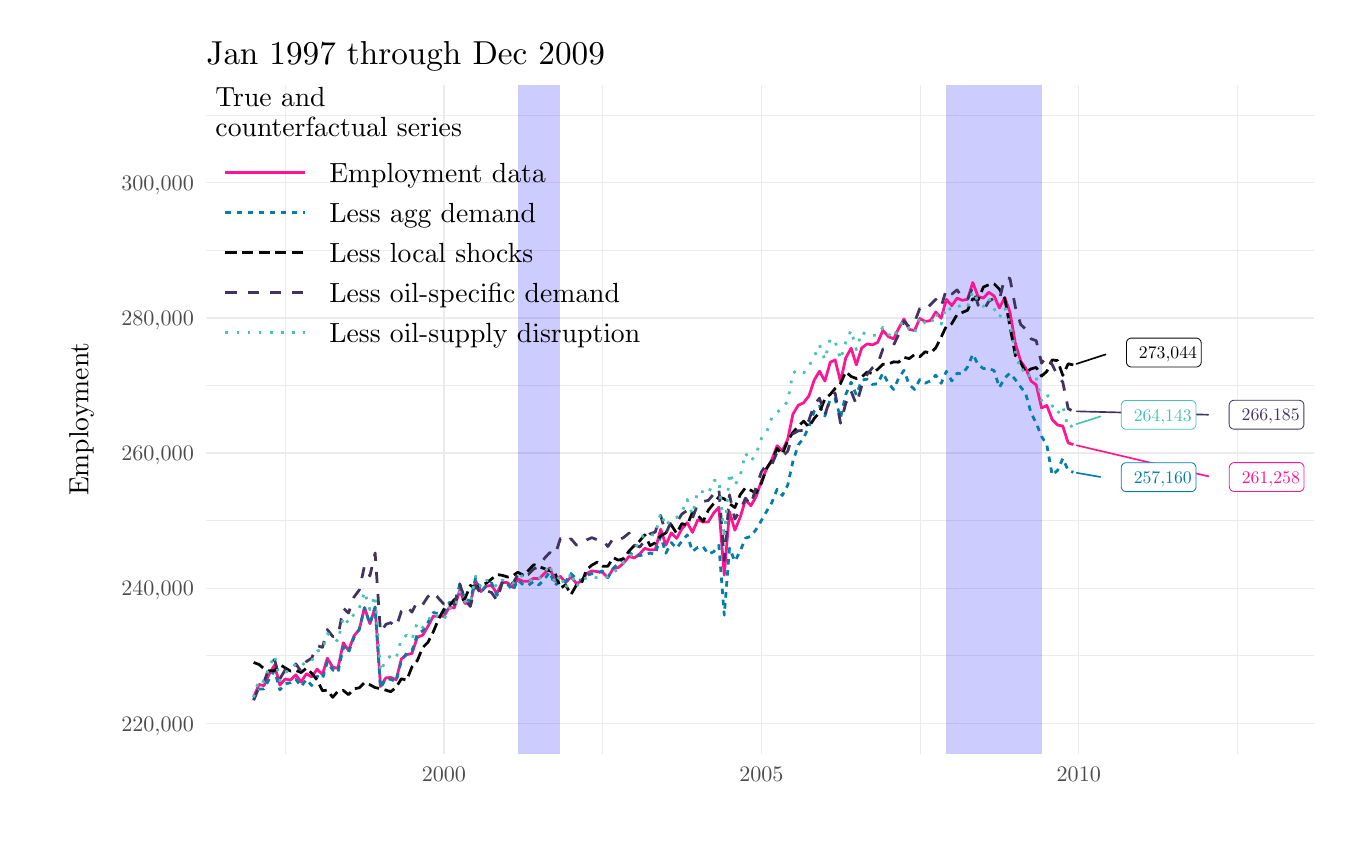
\begin{tikzpicture}[x=1pt,y=1pt]
\definecolor{fillColor}{RGB}{255,255,255}
\path[use as bounding box,fill=fillColor,fill opacity=0.00] (0,0) rectangle (469.75,290.32);
\begin{scope}
\path[clip] ( 64.55, 27.90) rectangle (464.75,269.73);
\definecolor{drawColor}{gray}{0.92}

\path[draw=drawColor,line width= 0.3pt,line join=round] ( 64.55, 63.32) --
	(464.75, 63.32);

\path[draw=drawColor,line width= 0.3pt,line join=round] ( 64.55,112.17) --
	(464.75,112.17);

\path[draw=drawColor,line width= 0.3pt,line join=round] ( 64.55,161.03) --
	(464.75,161.03);

\path[draw=drawColor,line width= 0.3pt,line join=round] ( 64.55,209.88) --
	(464.75,209.88);

\path[draw=drawColor,line width= 0.3pt,line join=round] ( 64.55,258.73) --
	(464.75,258.73);

\path[draw=drawColor,line width= 0.3pt,line join=round] ( 93.08, 27.90) --
	( 93.08,269.73);

\path[draw=drawColor,line width= 0.3pt,line join=round] (207.78, 27.90) --
	(207.78,269.73);

\path[draw=drawColor,line width= 0.3pt,line join=round] (322.48, 27.90) --
	(322.48,269.73);

\path[draw=drawColor,line width= 0.3pt,line join=round] (437.15, 27.90) --
	(437.15,269.73);

\path[draw=drawColor,line width= 0.5pt,line join=round] ( 64.55, 38.89) --
	(464.75, 38.89);

\path[draw=drawColor,line width= 0.5pt,line join=round] ( 64.55, 87.74) --
	(464.75, 87.74);

\path[draw=drawColor,line width= 0.5pt,line join=round] ( 64.55,136.60) --
	(464.75,136.60);

\path[draw=drawColor,line width= 0.5pt,line join=round] ( 64.55,185.45) --
	(464.75,185.45);

\path[draw=drawColor,line width= 0.5pt,line join=round] ( 64.55,234.31) --
	(464.75,234.31);

\path[draw=drawColor,line width= 0.5pt,line join=round] (150.41, 27.90) --
	(150.41,269.73);

\path[draw=drawColor,line width= 0.5pt,line join=round] (265.14, 27.90) --
	(265.14,269.73);

\path[draw=drawColor,line width= 0.5pt,line join=round] (379.81, 27.90) --
	(379.81,269.73);
\definecolor{fillColor}{RGB}{0,0,255}

\path[fill=fillColor,fill opacity=0.20] (177.10, 27.90) rectangle (192.49,269.73);

\path[fill=fillColor,fill opacity=0.20] (331.96, 27.90) rectangle (366.37,269.73);
\definecolor{drawColor}{RGB}{255,20,147}

\path[draw=drawColor,line width= 1.0pt,line join=round] ( 81.65, 48.45) --
	( 83.60, 52.99) --
	( 85.36, 52.53) --
	( 87.30, 56.81) --
	( 89.19, 59.97) --
	( 91.13, 52.75) --
	( 93.02, 54.97) --
	( 94.96, 54.56) --
	( 96.91, 56.49) --
	( 98.79, 53.88) --
	(100.74, 56.89) --
	(102.62, 55.71) --
	(104.57, 58.50) --
	(106.52, 56.53) --
	(108.28, 62.49) --
	(110.22, 59.23) --
	(112.11, 58.82) --
	(114.05, 68.05) --
	(115.94, 65.28) --
	(117.88, 70.46) --
	(119.83, 72.93) --
	(121.71, 80.76) --
	(123.66, 74.95) --
	(125.55, 80.77) --
	(127.49, 52.28) --
	(129.44, 55.40) --
	(131.20, 55.50) --
	(133.14, 54.69) --
	(135.03, 62.21) --
	(136.97, 63.75) --
	(138.86, 64.21) --
	(140.81, 70.06) --
	(142.75, 70.82) --
	(144.64, 73.98) --
	(146.58, 77.69) --
	(148.47, 77.62) --
	(150.41, 77.59) --
	(152.36, 80.88) --
	(154.18, 80.62) --
	(156.13, 87.01) --
	(158.01, 82.28) --
	(159.96, 82.37) --
	(161.84, 90.45) --
	(163.79, 86.55) --
	(165.74, 88.49) --
	(167.62, 88.80) --
	(169.57, 85.87) --
	(171.45, 89.97) --
	(173.40, 89.76) --
	(175.34, 88.06) --
	(177.10, 91.12) --
	(179.05, 90.27) --
	(180.93, 90.28) --
	(182.88, 91.35) --
	(184.76, 91.19) --
	(186.71, 93.06) --
	(188.66, 95.12) --
	(190.54, 90.37) --
	(192.49, 92.04) --
	(194.37, 89.81) --
	(196.32, 91.84) --
	(198.26, 89.52) --
	(200.02, 90.20) --
	(201.97, 93.04) --
	(203.85, 94.04) --
	(205.80, 93.76) --
	(207.68, 93.52) --
	(209.63, 91.56) --
	(211.58, 94.88) --
	(213.46, 95.25) --
	(215.41, 96.92) --
	(217.29, 99.26) --
	(219.24, 98.69) --
	(221.19,100.22) --
	(222.94,102.17) --
	(224.89,101.60) --
	(226.78,101.70) --
	(228.72,109.10) --
	(230.61,103.35) --
	(232.55,107.75) --
	(234.50,105.77) --
	(236.38,109.18) --
	(238.33,111.46) --
	(240.21,107.97) --
	(242.16,112.50) --
	(244.11,111.67) --
	(245.93,111.72) --
	(247.87,114.90) --
	(249.76,117.03) --
	(251.71, 92.50) --
	(253.59,115.42) --
	(255.54,108.73) --
	(257.48,113.44) --
	(259.37,119.71) --
	(261.31,117.57) --
	(263.20,120.79) --
	(265.14,126.55) --
	(267.09,131.04) --
	(268.85,134.13) --
	(270.80,139.25) --
	(272.68,137.41) --
	(274.63,141.54) --
	(276.51,150.65) --
	(278.46,153.88) --
	(280.40,154.79) --
	(282.29,157.24) --
	(284.23,162.99) --
	(286.12,166.18) --
	(288.07,162.61) --
	(290.01,169.42) --
	(291.77,170.25) --
	(293.72,162.40) --
	(295.60,170.93) --
	(297.55,174.52) --
	(299.43,168.47) --
	(301.38,174.57) --
	(303.33,176.06) --
	(305.21,175.70) --
	(307.16,176.60) --
	(309.04,180.95) --
	(310.99,178.66) --
	(312.93,177.87) --
	(314.69,181.61) --
	(316.64,185.05) --
	(318.52,181.30) --
	(320.47,180.88) --
	(322.35,185.23) --
	(324.30,184.16) --
	(326.25,184.47) --
	(328.13,187.59) --
	(330.08,185.32) --
	(331.96,192.16) --
	(333.91,189.87) --
	(335.85,192.59) --
	(337.68,191.82) --
	(339.62,192.14) --
	(341.51,198.25) --
	(343.45,193.14) --
	(345.34,192.61) --
	(347.28,194.71) --
	(349.23,193.37) --
	(351.11,189.03) --
	(353.06,192.77) --
	(354.94,187.55) --
	(356.89,176.28) --
	(358.84,169.76) --
	(360.60,167.33) --
	(362.54,162.66) --
	(364.43,161.24) --
	(366.37,152.90) --
	(368.26,153.79) --
	(370.20,148.75) --
	(372.15,146.74) --
	(374.04,146.34) --
	(375.98,140.27) --
	(377.87,139.67);
\definecolor{drawColor}{RGB}{0,127,168}

\path[draw=drawColor,line width= 1.0pt,dash pattern=on 2pt off 2pt ,line join=round] ( 81.65, 47.69) --
	( 83.60, 51.39) --
	( 85.36, 51.39) --
	( 87.30, 54.97) --
	( 89.19, 58.03) --
	( 91.13, 51.01) --
	( 93.02, 53.25) --
	( 94.96, 53.58) --
	( 96.91, 54.87) --
	( 98.79, 52.25) --
	(100.74, 54.80) --
	(102.62, 52.61) --
	(104.57, 55.98) --
	(106.52, 55.05) --
	(108.28, 61.22) --
	(110.22, 58.24) --
	(112.11, 57.29) --
	(114.05, 66.55) --
	(115.94, 64.54) --
	(117.88, 69.92) --
	(119.83, 72.88) --
	(121.71, 80.76) --
	(123.66, 74.90) --
	(125.55, 81.00) --
	(127.49, 51.71) --
	(129.44, 55.13) --
	(131.20, 54.82) --
	(133.14, 54.02) --
	(135.03, 61.63) --
	(136.97, 64.33) --
	(138.86, 65.14) --
	(140.81, 71.15) --
	(142.75, 72.38) --
	(144.64, 75.37) --
	(146.58, 78.99) --
	(148.47, 78.59) --
	(150.41, 78.82) --
	(152.36, 82.65) --
	(154.18, 82.08) --
	(156.13, 89.05) --
	(158.01, 83.73) --
	(159.96, 83.20) --
	(161.84, 91.47) --
	(163.79, 86.43) --
	(165.74, 88.84) --
	(167.62, 89.68) --
	(169.57, 85.17) --
	(171.45, 89.64) --
	(173.40, 89.21) --
	(175.34, 86.89) --
	(177.10, 90.72) --
	(179.05, 88.99) --
	(180.93, 88.86) --
	(182.88, 90.22) --
	(184.76, 88.96) --
	(186.71, 90.99) --
	(188.66, 93.61) --
	(190.54, 88.78) --
	(192.49, 90.78) --
	(194.37, 90.09) --
	(196.32, 93.08) --
	(198.26, 91.02) --
	(200.02, 90.59) --
	(201.97, 92.42) --
	(203.85, 92.99) --
	(205.80, 93.21) --
	(207.68, 94.02) --
	(209.63, 91.65) --
	(211.58, 94.96) --
	(213.46, 96.80) --
	(215.41, 98.71) --
	(217.29,100.82) --
	(219.24, 99.26) --
	(221.19, 99.58) --
	(222.94, 99.89) --
	(224.89,100.45) --
	(226.78,100.04) --
	(228.72,106.59) --
	(230.61,100.43) --
	(232.55,104.23) --
	(234.50,102.23) --
	(236.38,104.75) --
	(238.33,107.04) --
	(240.21,101.07) --
	(242.16,102.55) --
	(244.11,102.74) --
	(245.93,100.08) --
	(247.87,100.94) --
	(249.76,103.28) --
	(251.71, 78.01) --
	(253.59,102.22) --
	(255.54, 97.50) --
	(257.48,101.20) --
	(259.37,105.86) --
	(261.31,106.50) --
	(263.20,108.98) --
	(265.14,112.26) --
	(267.09,115.69) --
	(268.85,118.62) --
	(270.80,123.53) --
	(272.68,121.28) --
	(274.63,124.98) --
	(276.51,133.58) --
	(278.46,139.56) --
	(280.40,142.05) --
	(282.29,146.16) --
	(284.23,151.82) --
	(286.12,153.50) --
	(288.07,149.97) --
	(290.01,156.07) --
	(291.77,156.12) --
	(293.72,149.32) --
	(295.60,157.73) --
	(297.55,162.22) --
	(299.43,157.63) --
	(301.38,162.94) --
	(303.33,163.32) --
	(305.21,161.40) --
	(307.16,161.68) --
	(309.04,165.56) --
	(310.99,161.81) --
	(312.93,159.59) --
	(314.69,163.59) --
	(316.64,166.50) --
	(318.52,161.33) --
	(320.47,159.60) --
	(322.35,163.14) --
	(324.30,161.89) --
	(326.25,162.67) --
	(328.13,164.76) --
	(330.08,161.80) --
	(331.96,166.15) --
	(333.91,162.68) --
	(335.85,165.44) --
	(337.68,165.19) --
	(339.62,167.68) --
	(341.51,172.31) --
	(343.45,168.55) --
	(345.34,167.15) --
	(347.28,167.22) --
	(349.23,166.38) --
	(351.11,160.27) --
	(353.06,163.74) --
	(354.94,165.48) --
	(356.89,163.14) --
	(358.84,160.44) --
	(360.60,158.23) --
	(362.54,151.19) --
	(364.43,147.40) --
	(366.37,142.62) --
	(368.26,139.55) --
	(370.20,128.65) --
	(372.15,130.35) --
	(374.04,134.64) --
	(375.98,130.34) --
	(377.87,129.66);
\definecolor{drawColor}{RGB}{7,7,7}

\path[draw=drawColor,line width= 1.0pt,dash pattern=on 4pt off 2pt ,line join=round] ( 81.65, 60.94) --
	( 83.60, 60.21) --
	( 85.36, 58.74) --
	( 87.30, 57.89) --
	( 89.19, 57.97) --
	( 91.13, 60.14) --
	( 93.02, 59.01) --
	( 94.96, 57.83) --
	( 96.91, 58.08) --
	( 98.79, 57.27) --
	(100.74, 58.91) --
	(102.62, 57.05) --
	(104.57, 54.68) --
	(106.52, 50.73) --
	(108.28, 50.93) --
	(110.22, 48.33) --
	(112.11, 50.56) --
	(114.05, 50.83) --
	(115.94, 49.29) --
	(117.88, 51.40) --
	(119.83, 51.80) --
	(121.71, 53.64) --
	(123.66, 52.90) --
	(125.55, 51.85) --
	(127.49, 51.47) --
	(129.44, 50.94) --
	(131.20, 50.38) --
	(133.14, 51.94) --
	(135.03, 55.04) --
	(136.97, 54.56) --
	(138.86, 59.33) --
	(140.81, 61.66) --
	(142.75, 66.34) --
	(144.64, 68.22) --
	(146.58, 72.03) --
	(148.47, 76.61) --
	(150.41, 80.17) --
	(152.36, 81.44) --
	(154.18, 83.72) --
	(156.13, 82.91) --
	(158.01, 84.01) --
	(159.96, 88.75) --
	(161.84, 87.89) --
	(163.79, 89.02) --
	(165.74, 89.58) --
	(167.62, 91.11) --
	(169.57, 92.72) --
	(171.45, 92.44) --
	(173.40, 91.81) --
	(175.34, 92.28) --
	(177.10, 93.54) --
	(179.05, 92.47) --
	(180.93, 94.18) --
	(182.88, 96.27) --
	(184.76, 95.58) --
	(186.71, 94.85) --
	(188.66, 94.03) --
	(190.54, 93.45) --
	(192.49, 87.80) --
	(194.37, 88.98) --
	(196.32, 85.45) --
	(198.26, 88.86) --
	(200.02, 89.33) --
	(201.97, 94.47) --
	(203.85, 96.09) --
	(205.80, 97.19) --
	(207.68, 95.73) --
	(209.63, 95.69) --
	(211.58, 98.80) --
	(213.46, 97.90) --
	(215.41, 98.46) --
	(217.29,101.18) --
	(219.24,103.22) --
	(221.19,104.89) --
	(222.94,107.07) --
	(224.89,103.14) --
	(226.78,104.22) --
	(228.72,106.68) --
	(230.61,107.74) --
	(232.55,110.68) --
	(234.50,107.56) --
	(236.38,111.11) --
	(238.33,110.59) --
	(240.21,115.17) --
	(242.16,114.05) --
	(244.11,111.93) --
	(245.93,115.92) --
	(247.87,118.34) --
	(249.76,120.74) --
	(251.71,120.08) --
	(253.59,118.31) --
	(255.54,116.90) --
	(257.48,121.57) --
	(259.37,124.07) --
	(261.31,123.15) --
	(263.20,122.14) --
	(265.14,125.75) --
	(267.09,131.25) --
	(268.85,133.73) --
	(270.80,138.26) --
	(272.68,136.19) --
	(274.63,141.04) --
	(276.51,144.05) --
	(278.46,146.28) --
	(280.40,148.14) --
	(282.29,145.99) --
	(284.23,149.12) --
	(286.12,151.24) --
	(288.07,156.21) --
	(290.01,157.80) --
	(291.77,159.92) --
	(293.72,161.70) --
	(295.60,166.01) --
	(297.55,164.29) --
	(299.43,163.54) --
	(301.38,164.08) --
	(303.33,165.87) --
	(305.21,165.35) --
	(307.16,166.89) --
	(309.04,168.70) --
	(310.99,168.77) --
	(312.93,169.57) --
	(314.69,169.43) --
	(316.64,171.20) --
	(318.52,170.74) --
	(320.47,172.18) --
	(322.35,171.40) --
	(324.30,173.20) --
	(326.25,172.73) --
	(328.13,174.61) --
	(330.08,178.47) --
	(331.96,182.48) --
	(333.91,183.34) --
	(335.85,186.68) --
	(337.68,187.39) --
	(339.62,188.21) --
	(341.51,192.37) --
	(343.45,191.95) --
	(345.34,196.59) --
	(347.28,197.42) --
	(349.23,197.74) --
	(351.11,195.85) --
	(353.06,192.53) --
	(354.94,182.35) --
	(356.89,171.92) --
	(358.84,169.35) --
	(360.60,165.73) --
	(362.54,167.01) --
	(364.43,167.55) --
	(366.37,164.42) --
	(368.26,166.11) --
	(370.20,170.27) --
	(372.15,170.01) --
	(374.04,164.66) --
	(375.98,168.85) --
	(377.87,168.46);
\definecolor{drawColor}{RGB}{66,52,96}

\path[draw=drawColor,line width= 1.0pt,dash pattern=on 4pt off 4pt ,line join=round] ( 81.65, 47.28) --
	( 83.60, 52.06) --
	( 85.36, 53.70) --
	( 87.30, 59.33) --
	( 89.19, 62.03) --
	( 91.13, 55.02) --
	( 93.02, 58.24) --
	( 94.96, 57.85) --
	( 96.91, 60.43) --
	( 98.79, 57.71) --
	(100.74, 61.31) --
	(102.62, 62.49) --
	(104.57, 67.01) --
	(106.52, 66.40) --
	(108.28, 72.84) --
	(110.22, 70.34) --
	(112.11, 70.35) --
	(114.05, 80.55) --
	(115.94, 78.80) --
	(117.88, 84.52) --
	(119.83, 87.15) --
	(121.71, 95.87) --
	(123.66, 92.20) --
	(125.55,100.46) --
	(127.49, 71.83) --
	(129.44, 74.72) --
	(131.20, 75.33) --
	(133.14, 73.68) --
	(135.03, 79.44) --
	(136.97, 81.24) --
	(138.86, 79.12) --
	(140.81, 83.03) --
	(142.75, 81.84) --
	(144.64, 84.76) --
	(146.58, 86.48) --
	(148.47, 84.12) --
	(150.41, 82.00) --
	(152.36, 83.25) --
	(154.18, 81.82) --
	(156.13, 89.37) --
	(158.01, 83.57) --
	(159.96, 81.17) --
	(161.84, 88.75) --
	(163.79, 85.66) --
	(165.74, 86.85) --
	(167.62, 86.20) --
	(169.57, 83.37) --
	(171.45, 89.67) --
	(173.40, 91.43) --
	(175.34, 89.50) --
	(177.10, 92.66) --
	(179.05, 92.35) --
	(180.93, 92.77) --
	(182.88, 94.76) --
	(184.76, 95.50) --
	(186.71, 98.55) --
	(188.66,100.65) --
	(190.54, 99.66) --
	(192.49,105.71) --
	(194.37,104.40) --
	(196.32,105.65) --
	(198.26,103.37) --
	(200.02,103.35) --
	(201.97,105.22) --
	(203.85,106.04) --
	(205.80,105.28) --
	(207.68,105.44) --
	(209.63,102.81) --
	(211.58,105.75) --
	(213.46,105.06) --
	(215.41,106.14) --
	(217.29,107.70) --
	(219.24,103.39) --
	(221.19,102.65) --
	(222.94,104.95) --
	(224.89,107.42) --
	(226.78,108.06) --
	(228.72,114.07) --
	(230.61,107.48) --
	(232.55,111.98) --
	(234.50,111.50) --
	(236.38,114.56) --
	(238.33,115.85) --
	(240.21,112.98) --
	(242.16,118.36) --
	(244.11,119.11) --
	(245.93,119.49) --
	(247.87,121.75) --
	(249.76,123.77) --
	(251.71, 97.80) --
	(253.59,121.52) --
	(255.54,112.77) --
	(257.48,115.91) --
	(259.37,120.31) --
	(261.31,117.86) --
	(263.20,124.29) --
	(265.14,129.81) --
	(267.09,132.72) --
	(268.85,132.31) --
	(270.80,136.92) --
	(272.68,135.38) --
	(274.63,137.23) --
	(276.51,143.53) --
	(278.46,144.64) --
	(280.40,144.78) --
	(282.29,148.47) --
	(284.23,154.07) --
	(286.12,156.43) --
	(288.07,150.41) --
	(290.01,156.27) --
	(291.77,158.29) --
	(293.72,147.40) --
	(295.60,154.52) --
	(297.55,158.94) --
	(299.43,154.18) --
	(301.38,160.88) --
	(303.33,165.03) --
	(305.21,167.39) --
	(307.16,168.86) --
	(309.04,174.18) --
	(310.99,174.36) --
	(312.93,175.66) --
	(314.69,179.39) --
	(316.64,184.25) --
	(318.52,182.25) --
	(320.47,183.85) --
	(322.35,188.84) --
	(324.30,188.21) --
	(326.25,190.28) --
	(328.13,192.14) --
	(330.08,189.44) --
	(331.96,195.80) --
	(333.91,194.03) --
	(335.85,195.57) --
	(337.68,192.88) --
	(339.62,192.07) --
	(341.51,196.57) --
	(343.45,190.05) --
	(345.34,188.08) --
	(347.28,191.42) --
	(349.23,192.59) --
	(351.11,191.89) --
	(353.06,200.02) --
	(354.94,199.74) --
	(356.89,189.36) --
	(358.84,183.03) --
	(360.60,181.41) --
	(362.54,177.89) --
	(364.43,177.21) --
	(366.37,169.07) --
	(368.26,171.57) --
	(370.20,168.55) --
	(372.15,164.60) --
	(374.04,162.24) --
	(375.98,152.63) --
	(377.87,151.71);
\definecolor{drawColor}{RGB}{72,194,180}

\path[draw=drawColor,line width= 1.0pt,dash pattern=on 1pt off 3pt ,line join=round] ( 81.65, 48.34) --
	( 83.60, 54.88) --
	( 85.36, 54.00) --
	( 87.30, 59.19) --
	( 89.19, 63.54) --
	( 91.13, 54.39) --
	( 93.02, 57.40) --
	( 94.96, 58.10) --
	( 96.91, 60.49) --
	( 98.79, 59.49) --
	(100.74, 61.48) --
	(102.62, 61.52) --
	(104.57, 65.11) --
	(106.52, 65.42) --
	(108.28, 71.38) --
	(110.22, 70.40) --
	(112.11, 68.50) --
	(114.05, 77.48) --
	(115.94, 75.17) --
	(117.88, 78.34) --
	(119.83, 80.54) --
	(121.71, 86.51) --
	(123.66, 79.99) --
	(125.55, 85.16) --
	(127.49, 57.60) --
	(129.44, 62.01) --
	(131.20, 63.32) --
	(133.14, 62.38) --
	(135.03, 69.42) --
	(136.97, 70.81) --
	(138.86, 69.28) --
	(140.81, 75.42) --
	(142.75, 73.60) --
	(144.64, 76.06) --
	(146.58, 78.76) --
	(148.47, 77.40) --
	(150.41, 76.32) --
	(152.36, 80.57) --
	(154.18, 80.24) --
	(156.13, 86.46) --
	(158.01, 82.98) --
	(159.96, 82.17) --
	(161.84, 92.14) --
	(163.79, 88.15) --
	(165.74, 90.57) --
	(167.62, 90.52) --
	(169.57, 88.20) --
	(171.45, 90.74) --
	(173.40, 90.15) --
	(175.34, 89.56) --
	(177.10, 91.25) --
	(179.05, 92.53) --
	(180.93, 91.30) --
	(182.88, 89.83) --
	(184.76, 91.31) --
	(186.71, 93.32) --
	(188.66, 96.35) --
	(190.54, 89.25) --
	(192.49, 92.64) --
	(194.37, 87.48) --
	(196.32, 93.61) --
	(198.26, 88.19) --
	(200.02, 90.96) --
	(201.97, 91.41) --
	(203.85, 92.17) --
	(205.80, 91.49) --
	(207.68, 92.01) --
	(209.63, 91.86) --
	(211.58, 93.30) --
	(213.46, 94.86) --
	(215.41, 97.09) --
	(217.29, 98.51) --
	(219.24,101.34) --
	(221.19,105.44) --
	(222.94,107.31) --
	(224.89,107.21) --
	(226.78,106.96) --
	(228.72,115.03) --
	(230.61,110.15) --
	(232.55,112.94) --
	(234.50,113.35) --
	(236.38,115.26) --
	(238.33,119.86) --
	(240.21,114.35) --
	(242.16,123.06) --
	(244.11,122.53) --
	(245.93,121.76) --
	(247.87,126.62) --
	(249.76,127.03) --
	(251.71,106.06) --
	(253.59,129.46) --
	(255.54,124.95) --
	(257.48,128.45) --
	(259.37,136.61) --
	(261.31,133.61) --
	(263.20,136.15) --
	(265.14,141.91) --
	(267.09,144.33) --
	(268.85,149.42) --
	(270.80,151.41) --
	(272.68,152.66) --
	(274.63,155.41) --
	(276.51,165.56) --
	(278.46,166.60) --
	(280.40,165.55) --
	(282.29,167.97) --
	(284.23,171.49) --
	(286.12,175.68) --
	(288.07,170.35) --
	(290.01,177.92) --
	(291.77,176.98) --
	(293.72,170.42) --
	(295.60,176.72) --
	(297.55,181.00) --
	(299.43,173.94) --
	(301.38,180.35) --
	(303.33,179.23) --
	(305.21,179.08) --
	(307.16,179.28) --
	(309.04,182.02) --
	(310.99,179.58) --
	(312.93,178.22) --
	(314.69,182.58) --
	(316.64,184.10) --
	(318.52,181.50) --
	(320.47,179.79) --
	(322.35,185.88) --
	(324.30,183.59) --
	(326.25,182.99) --
	(328.13,187.30) --
	(330.08,183.14) --
	(331.96,189.63) --
	(333.91,188.16) --
	(335.85,189.40) --
	(337.68,190.16) --
	(339.62,189.40) --
	(341.51,195.07) --
	(343.45,191.50) --
	(345.34,189.59) --
	(347.28,192.47) --
	(349.23,188.71) --
	(351.11,185.55) --
	(353.06,189.17) --
	(354.94,183.07) --
	(356.89,173.29) --
	(358.84,166.18) --
	(360.60,167.16) --
	(362.54,163.30) --
	(364.43,163.86) --
	(366.37,155.57) --
	(368.26,158.06) --
	(370.20,153.75) --
	(372.15,150.83) --
	(374.04,153.54) --
	(375.98,145.73) --
	(377.87,146.72);
\end{scope}
\begin{scope}
\path[clip] ( 64.55, 27.90) rectangle (464.75,269.73);
\definecolor{drawColor}{RGB}{255,20,147}

\path[draw=drawColor,line width= 0.6pt,line join=round,line cap=round] (426.69,128.19) -- (378.99,139.41);
\definecolor{drawColor}{RGB}{72,194,180}

\path[draw=drawColor,line width= 0.6pt,line join=round,line cap=round] (387.63,149.84) -- (378.93,147.06);
\definecolor{drawColor}{RGB}{0,127,168}

\path[draw=drawColor,line width= 0.6pt,line join=round,line cap=round] (387.64,127.97) -- (379.03,129.46);
\definecolor{drawColor}{RGB}{66,52,96}

\path[draw=drawColor,line width= 0.6pt,line join=round,line cap=round] (426.62,150.46) -- (379.07,151.68);
\definecolor{drawColor}{RGB}{7,7,7}

\path[draw=drawColor,line width= 0.6pt,line join=round,line cap=round] (389.51,172.24) -- (378.93,168.81);
\definecolor{drawColor}{RGB}{255,20,147}
\definecolor{fillColor}{RGB}{255,255,255}

\path[draw=drawColor,line width= 0.3pt,line join=round,line cap=round,fill=fillColor] (436.02,122.72) --
	(459.41,122.72) --
	(459.34,122.72) --
	(459.63,122.73) --
	(459.91,122.79) --
	(460.18,122.89) --
	(460.43,123.04) --
	(460.66,123.22) --
	(460.85,123.44) --
	(461.01,123.69) --
	(461.12,123.95) --
	(461.19,124.24) --
	(461.22,124.53) --
	(461.22,124.53) --
	(461.22,131.35) --
	(461.22,131.35) --
	(461.19,131.63) --
	(461.12,131.92) --
	(461.01,132.18) --
	(460.85,132.43) --
	(460.66,132.65) --
	(460.43,132.83) --
	(460.18,132.98) --
	(459.91,133.08) --
	(459.63,133.14) --
	(459.41,133.15) --
	(436.02,133.15) --
	(436.24,133.14) --
	(435.95,133.15) --
	(435.66,133.12) --
	(435.38,133.03) --
	(435.12,132.91) --
	(434.88,132.74) --
	(434.67,132.54) --
	(434.49,132.31) --
	(434.36,132.05) --
	(434.27,131.78) --
	(434.22,131.49) --
	(434.21,131.35) --
	(434.21,124.53) --
	(434.22,124.67) --
	(434.22,124.38) --
	(434.27,124.09) --
	(434.36,123.82) --
	(434.49,123.56) --
	(434.67,123.33) --
	(434.88,123.13) --
	(435.12,122.96) --
	(435.38,122.84) --
	(435.66,122.76) --
	(435.95,122.72) --
	cycle;
\end{scope}
\begin{scope}
\path[clip] ( 64.55, 27.90) rectangle (464.75,269.73);
\definecolor{drawColor}{RGB}{255,20,147}

\node[text=drawColor,anchor=base east,inner sep=0pt, outer sep=0pt, scale=  0.64] at (459.71,125.73) {261,258};
\definecolor{drawColor}{RGB}{72,194,180}
\definecolor{fillColor}{RGB}{255,255,255}

\path[draw=drawColor,line width= 0.3pt,line join=round,line cap=round,fill=fillColor] (396.97,145.18) --
	(420.36,145.18) --
	(420.28,145.18) --
	(420.58,145.19) --
	(420.86,145.25) --
	(421.13,145.36) --
	(421.38,145.50) --
	(421.61,145.68) --
	(421.80,145.90) --
	(421.96,146.15) --
	(422.07,146.42) --
	(422.14,146.70) --
	(422.16,146.99) --
	(422.16,146.99) --
	(422.16,153.81) --
	(422.16,153.81) --
	(422.14,154.10) --
	(422.07,154.38) --
	(421.96,154.65) --
	(421.80,154.89) --
	(421.61,155.11) --
	(421.38,155.29) --
	(421.13,155.44) --
	(420.86,155.54) --
	(420.58,155.60) --
	(420.36,155.61) --
	(396.97,155.61) --
	(397.19,155.60) --
	(396.90,155.61) --
	(396.61,155.58) --
	(396.33,155.50) --
	(396.07,155.37) --
	(395.83,155.21) --
	(395.62,155.00) --
	(395.44,154.77) --
	(395.31,154.51) --
	(395.22,154.24) --
	(395.17,153.95) --
	(395.16,153.81) --
	(395.16,146.99) --
	(395.17,147.13) --
	(395.17,146.84) --
	(395.22,146.56) --
	(395.31,146.28) --
	(395.44,146.02) --
	(395.62,145.79) --
	(395.83,145.59) --
	(396.07,145.42) --
	(396.33,145.30) --
	(396.61,145.22) --
	(396.90,145.18) --
	cycle;
\end{scope}
\begin{scope}
\path[clip] ( 64.55, 27.90) rectangle (464.75,269.73);
\definecolor{drawColor}{RGB}{72,194,180}

\node[text=drawColor,anchor=base east,inner sep=0pt, outer sep=0pt, scale=  0.64] at (420.66,148.19) {264,143};
\definecolor{drawColor}{RGB}{0,127,168}
\definecolor{fillColor}{RGB}{255,255,255}

\path[draw=drawColor,line width= 0.3pt,line join=round,line cap=round,fill=fillColor] (396.97,122.68) --
	(420.36,122.68) --
	(420.29,122.68) --
	(420.58,122.69) --
	(420.86,122.75) --
	(421.13,122.85) --
	(421.39,123.00) --
	(421.61,123.18) --
	(421.80,123.40) --
	(421.96,123.64) --
	(422.07,123.91) --
	(422.14,124.19) --
	(422.17,124.48) --
	(422.17,124.48) --
	(422.17,131.30) --
	(422.17,131.30) --
	(422.14,131.59) --
	(422.07,131.87) --
	(421.96,132.14) --
	(421.80,132.39) --
	(421.61,132.60) --
	(421.39,132.79) --
	(421.13,132.93) --
	(420.86,133.04) --
	(420.58,133.10) --
	(420.36,133.11) --
	(396.97,133.11) --
	(397.19,133.10) --
	(396.90,133.11) --
	(396.61,133.07) --
	(396.33,132.99) --
	(396.07,132.87) --
	(395.83,132.70) --
	(395.62,132.50) --
	(395.44,132.27) --
	(395.31,132.01) --
	(395.22,131.73) --
	(395.17,131.45) --
	(395.16,131.30) --
	(395.16,124.48) --
	(395.17,124.63) --
	(395.17,124.34) --
	(395.22,124.05) --
	(395.31,123.78) --
	(395.44,123.52) --
	(395.62,123.29) --
	(395.83,123.08) --
	(396.07,122.92) --
	(396.33,122.79) --
	(396.61,122.71) --
	(396.90,122.68) --
	cycle;
\end{scope}
\begin{scope}
\path[clip] ( 64.55, 27.90) rectangle (464.75,269.73);
\definecolor{drawColor}{RGB}{0,127,168}

\node[text=drawColor,anchor=base east,inner sep=0pt, outer sep=0pt, scale=  0.64] at (420.66,125.69) {257,160};
\definecolor{drawColor}{RGB}{66,52,96}
\definecolor{fillColor}{RGB}{255,255,255}

\path[draw=drawColor,line width= 0.3pt,line join=round,line cap=round,fill=fillColor] (435.96,145.25) --
	(459.35,145.25) --
	(459.27,145.25) --
	(459.56,145.26) --
	(459.85,145.32) --
	(460.12,145.42) --
	(460.37,145.57) --
	(460.60,145.75) --
	(460.79,145.97) --
	(460.95,146.21) --
	(461.06,146.48) --
	(461.13,146.76) --
	(461.15,147.05) --
	(461.15,147.05) --
	(461.15,153.87) --
	(461.15,153.87) --
	(461.13,154.16) --
	(461.06,154.44) --
	(460.95,154.71) --
	(460.79,154.96) --
	(460.60,155.17) --
	(460.37,155.36) --
	(460.12,155.50) --
	(459.85,155.61) --
	(459.56,155.66) --
	(459.35,155.68) --
	(435.96,155.68) --
	(436.18,155.66) --
	(435.88,155.68) --
	(435.60,155.64) --
	(435.32,155.56) --
	(435.05,155.44) --
	(434.81,155.27) --
	(434.61,155.07) --
	(434.43,154.84) --
	(434.30,154.58) --
	(434.20,154.30) --
	(434.16,154.02) --
	(434.15,153.87) --
	(434.15,147.05) --
	(434.16,147.20) --
	(434.16,146.91) --
	(434.20,146.62) --
	(434.30,146.34) --
	(434.43,146.09) --
	(434.61,145.85) --
	(434.81,145.65) --
	(435.05,145.49) --
	(435.32,145.36) --
	(435.60,145.28) --
	(435.88,145.25) --
	cycle;
\end{scope}
\begin{scope}
\path[clip] ( 64.55, 27.90) rectangle (464.75,269.73);
\definecolor{drawColor}{RGB}{66,52,96}

\node[text=drawColor,anchor=base east,inner sep=0pt, outer sep=0pt, scale=  0.64] at (459.65,148.26) {266,185};
\definecolor{drawColor}{RGB}{7,7,7}
\definecolor{fillColor}{RGB}{255,255,255}

\path[draw=drawColor,line width= 0.3pt,line join=round,line cap=round,fill=fillColor] (398.85,167.72) --
	(422.24,167.72) --
	(422.17,167.72) --
	(422.46,167.73) --
	(422.74,167.79) --
	(423.01,167.89) --
	(423.26,168.04) --
	(423.49,168.22) --
	(423.68,168.44) --
	(423.84,168.68) --
	(423.95,168.95) --
	(424.02,169.23) --
	(424.04,169.52) --
	(424.04,169.52) --
	(424.04,176.34) --
	(424.04,176.34) --
	(424.02,176.63) --
	(423.95,176.91) --
	(423.84,177.18) --
	(423.68,177.43) --
	(423.49,177.64) --
	(423.26,177.83) --
	(423.01,177.97) --
	(422.74,178.08) --
	(422.46,178.13) --
	(422.24,178.15) --
	(398.85,178.15) --
	(399.07,178.13) --
	(398.78,178.15) --
	(398.49,178.11) --
	(398.21,178.03) --
	(397.95,177.91) --
	(397.71,177.74) --
	(397.50,177.54) --
	(397.32,177.31) --
	(397.19,177.05) --
	(397.10,176.77) --
	(397.05,176.49) --
	(397.04,176.34) --
	(397.04,169.52) --
	(397.05,169.67) --
	(397.05,169.38) --
	(397.10,169.09) --
	(397.19,168.82) --
	(397.32,168.56) --
	(397.50,168.33) --
	(397.71,168.12) --
	(397.95,167.96) --
	(398.21,167.83) --
	(398.49,167.75) --
	(398.78,167.72) --
	cycle;
\end{scope}
\begin{scope}
\path[clip] ( 64.55, 27.90) rectangle (464.75,269.73);
\definecolor{drawColor}{RGB}{7,7,7}

\node[text=drawColor,anchor=base east,inner sep=0pt, outer sep=0pt, scale=  0.64] at (422.54,170.73) {273,044};
\end{scope}
\begin{scope}
\path[clip] (  0.00,  0.00) rectangle (469.75,290.32);
\definecolor{drawColor}{gray}{0.30}

\node[text=drawColor,anchor=base east,inner sep=0pt, outer sep=0pt, scale=  0.80] at ( 60.05, 36.13) {220,000};

\node[text=drawColor,anchor=base east,inner sep=0pt, outer sep=0pt, scale=  0.80] at ( 60.05, 84.99) {240,000};

\node[text=drawColor,anchor=base east,inner sep=0pt, outer sep=0pt, scale=  0.80] at ( 60.05,133.84) {260,000};

\node[text=drawColor,anchor=base east,inner sep=0pt, outer sep=0pt, scale=  0.80] at ( 60.05,182.70) {280,000};

\node[text=drawColor,anchor=base east,inner sep=0pt, outer sep=0pt, scale=  0.80] at ( 60.05,231.55) {300,000};
\end{scope}
\begin{scope}
\path[clip] (  0.00,  0.00) rectangle (469.75,290.32);
\definecolor{drawColor}{gray}{0.30}

\node[text=drawColor,anchor=base,inner sep=0pt, outer sep=0pt, scale=  0.80] at (150.41, 17.89) {2000};

\node[text=drawColor,anchor=base,inner sep=0pt, outer sep=0pt, scale=  0.80] at (265.14, 17.89) {2005};

\node[text=drawColor,anchor=base,inner sep=0pt, outer sep=0pt, scale=  0.80] at (379.81, 17.89) {2010};
\end{scope}
\begin{scope}
\path[clip] (  0.00,  0.00) rectangle (469.75,290.32);
\definecolor{drawColor}{RGB}{0,0,0}

\node[text=drawColor,rotate= 90.00,anchor=base,inner sep=0pt, outer sep=0pt, scale=  1.00] at ( 21.89,148.81) {Employment};
\end{scope}
\begin{scope}
\path[clip] (  0.00,  0.00) rectangle (469.75,290.32);
\definecolor{drawColor}{RGB}{0,0,0}

\node[text=drawColor,anchor=base west,inner sep=0pt, outer sep=0pt, scale=  1.00] at ( 67.87,261.95) {True and};

\node[text=drawColor,anchor=base west,inner sep=0pt, outer sep=0pt, scale=  1.00] at ( 67.87,251.15) {counterfactual series};
\end{scope}
\begin{scope}
\path[clip] (  0.00,  0.00) rectangle (469.75,290.32);
\definecolor{drawColor}{RGB}{255,20,147}

\path[draw=drawColor,line width= 1.0pt,line join=round] ( 71.48,237.95) -- (100.39,237.95);
\end{scope}
\begin{scope}
\path[clip] (  0.00,  0.00) rectangle (469.75,290.32);
\definecolor{drawColor}{RGB}{0,127,168}

\path[draw=drawColor,line width= 1.0pt,dash pattern=on 2pt off 2pt ,line join=round] ( 71.48,223.50) -- (100.39,223.50);
\end{scope}
\begin{scope}
\path[clip] (  0.00,  0.00) rectangle (469.75,290.32);
\definecolor{drawColor}{RGB}{7,7,7}

\path[draw=drawColor,line width= 1.0pt,dash pattern=on 4pt off 2pt ,line join=round] ( 71.48,209.05) -- (100.39,209.05);
\end{scope}
\begin{scope}
\path[clip] (  0.00,  0.00) rectangle (469.75,290.32);
\definecolor{drawColor}{RGB}{66,52,96}

\path[draw=drawColor,line width= 1.0pt,dash pattern=on 4pt off 4pt ,line join=round] ( 71.48,194.59) -- (100.39,194.59);
\end{scope}
\begin{scope}
\path[clip] (  0.00,  0.00) rectangle (469.75,290.32);
\definecolor{drawColor}{RGB}{72,194,180}

\path[draw=drawColor,line width= 1.0pt,dash pattern=on 1pt off 3pt ,line join=round] ( 71.48,180.14) -- (100.39,180.14);
\end{scope}
\begin{scope}
\path[clip] (  0.00,  0.00) rectangle (469.75,290.32);
\definecolor{drawColor}{RGB}{0,0,0}

\node[text=drawColor,anchor=base west,inner sep=0pt, outer sep=0pt, scale=  1.00] at (109.00,234.51) {Employment data};
\end{scope}
\begin{scope}
\path[clip] (  0.00,  0.00) rectangle (469.75,290.32);
\definecolor{drawColor}{RGB}{0,0,0}

\node[text=drawColor,anchor=base west,inner sep=0pt, outer sep=0pt, scale=  1.00] at (109.00,220.06) {Less agg demand};
\end{scope}
\begin{scope}
\path[clip] (  0.00,  0.00) rectangle (469.75,290.32);
\definecolor{drawColor}{RGB}{0,0,0}

\node[text=drawColor,anchor=base west,inner sep=0pt, outer sep=0pt, scale=  1.00] at (109.00,205.60) {Less local shocks};
\end{scope}
\begin{scope}
\path[clip] (  0.00,  0.00) rectangle (469.75,290.32);
\definecolor{drawColor}{RGB}{0,0,0}

\node[text=drawColor,anchor=base west,inner sep=0pt, outer sep=0pt, scale=  1.00] at (109.00,191.15) {Less oil-specific demand};
\end{scope}
\begin{scope}
\path[clip] (  0.00,  0.00) rectangle (469.75,290.32);
\definecolor{drawColor}{RGB}{0,0,0}

\node[text=drawColor,anchor=base west,inner sep=0pt, outer sep=0pt, scale=  1.00] at (109.00,176.69) {Less oil-supply disruption};
\end{scope}
\begin{scope}
\path[clip] (  0.00,  0.00) rectangle (469.75,290.32);
\definecolor{drawColor}{RGB}{0,0,0}

\node[text=drawColor,anchor=base west,inner sep=0pt, outer sep=0pt, scale=  1.20] at ( 64.55,277.06) {Jan 1997 through Dec 2009};
\end{scope}
\end{tikzpicture}
}
\caption{Counterfactuals for employment, January $1997$ through December $2009$}
\end{figure}

\begin{figure}[htbp]
  \centering
  % \resizebox{<horizontal size>}{<vertical size>}{%
  \resizebox{\textwidth}{!}{
  % Created by tikzDevice version 0.12.6 on 2026-02-23 20:01:58
% !TEX encoding = UTF-8 Unicode
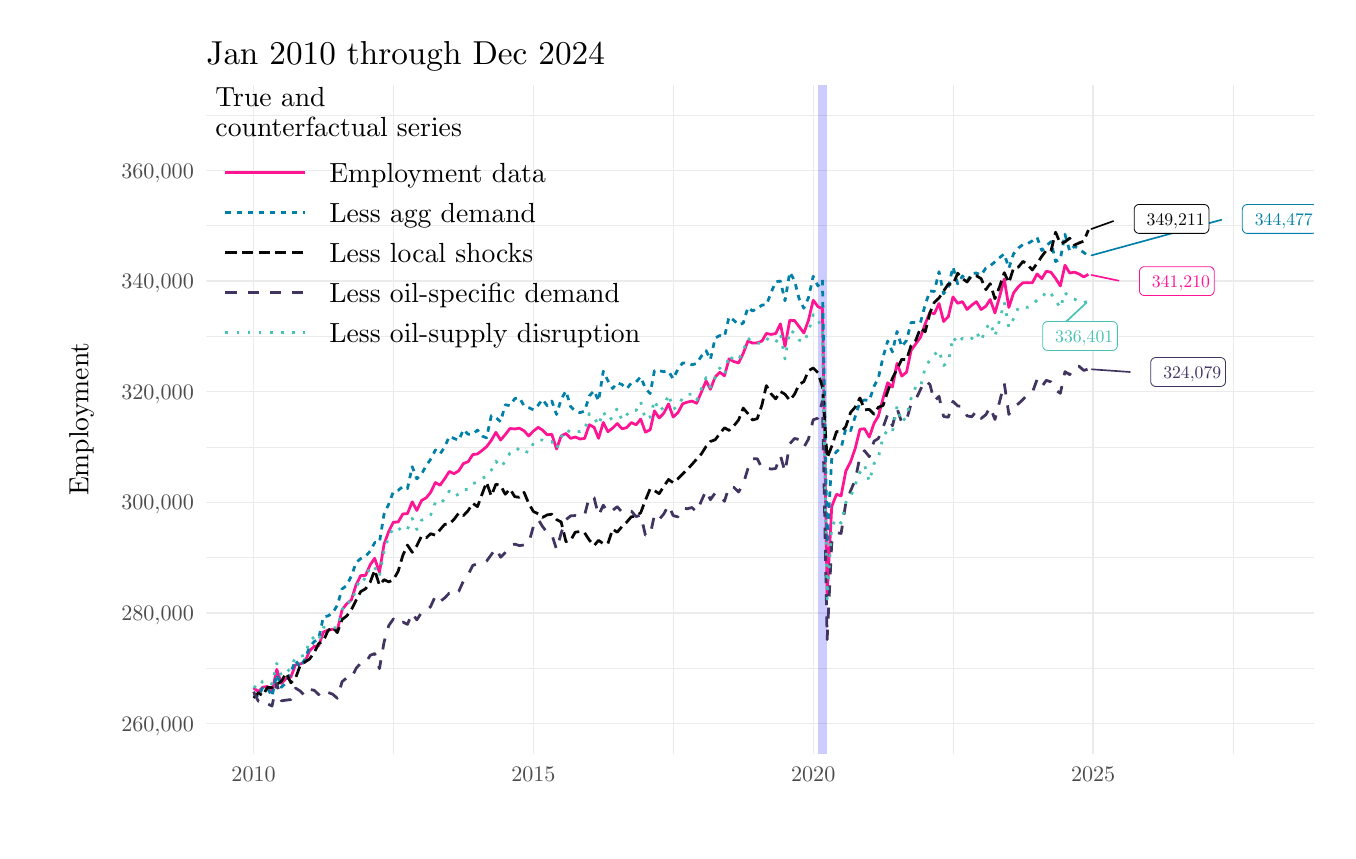
\begin{tikzpicture}[x=1pt,y=1pt]
\definecolor{fillColor}{RGB}{255,255,255}
\path[use as bounding box,fill=fillColor,fill opacity=0.00] (0,0) rectangle (469.75,290.32);
\begin{scope}
\path[clip] ( 64.55, 27.90) rectangle (464.75,269.73);
\definecolor{drawColor}{gray}{0.92}

\path[draw=drawColor,line width= 0.3pt,line join=round] ( 64.55, 58.87) --
	(464.75, 58.87);

\path[draw=drawColor,line width= 0.3pt,line join=round] ( 64.55, 98.85) --
	(464.75, 98.85);

\path[draw=drawColor,line width= 0.3pt,line join=round] ( 64.55,138.82) --
	(464.75,138.82);

\path[draw=drawColor,line width= 0.3pt,line join=round] ( 64.55,178.79) --
	(464.75,178.79);

\path[draw=drawColor,line width= 0.3pt,line join=round] ( 64.55,218.76) --
	(464.75,218.76);

\path[draw=drawColor,line width= 0.3pt,line join=round] ( 64.55,258.73) --
	(464.75,258.73);

\path[draw=drawColor,line width= 0.3pt,line join=round] (132.20, 27.90) --
	(132.20,269.73);

\path[draw=drawColor,line width= 0.3pt,line join=round] (233.30, 27.90) --
	(233.30,269.73);

\path[draw=drawColor,line width= 0.3pt,line join=round] (334.43, 27.90) --
	(334.43,269.73);

\path[draw=drawColor,line width= 0.3pt,line join=round] (435.56, 27.90) --
	(435.56,269.73);

\path[draw=drawColor,line width= 0.5pt,line join=round] ( 64.55, 38.89) --
	(464.75, 38.89);

\path[draw=drawColor,line width= 0.5pt,line join=round] ( 64.55, 78.86) --
	(464.75, 78.86);

\path[draw=drawColor,line width= 0.5pt,line join=round] ( 64.55,118.83) --
	(464.75,118.83);

\path[draw=drawColor,line width= 0.5pt,line join=round] ( 64.55,158.80) --
	(464.75,158.80);

\path[draw=drawColor,line width= 0.5pt,line join=round] ( 64.55,198.78) --
	(464.75,198.78);

\path[draw=drawColor,line width= 0.5pt,line join=round] ( 64.55,238.75) --
	(464.75,238.75);

\path[draw=drawColor,line width= 0.5pt,line join=round] ( 81.65, 27.90) --
	( 81.65,269.73);

\path[draw=drawColor,line width= 0.5pt,line join=round] (182.75, 27.90) --
	(182.75,269.73);

\path[draw=drawColor,line width= 0.5pt,line join=round] (283.85, 27.90) --
	(283.85,269.73);

\path[draw=drawColor,line width= 0.5pt,line join=round] (385.01, 27.90) --
	(385.01,269.73);
\definecolor{fillColor}{RGB}{0,0,255}

\path[fill=fillColor,fill opacity=0.20] (285.57, 27.90) rectangle (288.89,269.73);
\definecolor{drawColor}{RGB}{255,20,147}

\path[draw=drawColor,line width= 1.0pt,line join=round] ( 81.65, 51.73) --
	( 83.37, 50.34) --
	( 84.92, 51.98) --
	( 86.63, 52.28) --
	( 88.29, 50.32) --
	( 90.01, 58.43) --
	( 91.67, 53.37) --
	( 93.39, 55.11) --
	( 95.10, 55.65) --
	( 96.77, 60.11) --
	( 98.48, 60.40) --
	(100.14, 61.04) --
	(101.86, 65.17) --
	(103.58, 66.79) --
	(105.13, 66.92) --
	(106.84, 71.91) --
	(108.50, 72.61) --
	(110.22, 72.96) --
	(111.88, 72.48) --
	(113.60, 79.95) --
	(115.31, 82.18) --
	(116.97, 83.54) --
	(118.69, 89.07) --
	(120.35, 92.32) --
	(122.07, 92.40) --
	(123.78, 96.25) --
	(125.39, 98.58) --
	(127.11, 93.49) --
	(128.77,103.67) --
	(130.48,108.31) --
	(132.14,111.63) --
	(133.86,111.67) --
	(135.58,114.61) --
	(137.24,114.75) --
	(138.95,119.00) --
	(140.62,115.87) --
	(142.33,119.47) --
	(144.05,120.47) --
	(145.60,122.40) --
	(147.32,125.96) --
	(148.98,124.97) --
	(150.69,127.33) --
	(152.35,129.96) --
	(154.07,129.15) --
	(155.79,130.23) --
	(157.45,132.82) --
	(159.16,133.47) --
	(160.82,136.03) --
	(162.54,136.29) --
	(164.26,137.60) --
	(165.81,138.88) --
	(167.52,141.17) --
	(169.19,144.10) --
	(170.90,141.30) --
	(172.56,143.27) --
	(174.28,145.48) --
	(176.00,145.32) --
	(177.66,145.59) --
	(179.37,144.65) --
	(181.03,142.79) --
	(182.75,144.55) --
	(184.47,145.90) --
	(186.02,144.90) --
	(187.73,143.21) --
	(189.39,143.41) --
	(191.11,138.06) --
	(192.77,142.78) --
	(194.49,143.69) --
	(196.20,141.90) --
	(197.87,142.41) --
	(199.58,141.68) --
	(201.24,141.90) --
	(202.96,146.85) --
	(204.68,145.91) --
	(206.28,141.90) --
	(208.00,147.67) --
	(209.66,144.33) --
	(211.38,145.62) --
	(213.04,147.27) --
	(214.75,145.38) --
	(216.47,145.81) --
	(218.13,147.63) --
	(219.85,146.81) --
	(221.51,148.87) --
	(223.22,144.15) --
	(224.94,145.03) --
	(226.49,151.85) --
	(228.21,149.28) --
	(229.87,151.02) --
	(231.58,154.35) --
	(233.25,149.63) --
	(234.96,151.18) --
	(236.68,154.41) --
	(238.34,154.99) --
	(240.06,155.40) --
	(241.72,154.60) --
	(243.43,158.63) --
	(245.15,162.70) --
	(246.70,159.64) --
	(248.42,164.09) --
	(250.08,165.81) --
	(251.79,164.53) --
	(253.45,170.64) --
	(255.17,169.68) --
	(256.89,169.15) --
	(258.55,172.60) --
	(260.26,177.08) --
	(261.93,176.33) --
	(263.64,176.44) --
	(265.36,177.08) --
	(266.91,179.83) --
	(268.62,179.48) --
	(270.29,179.78) --
	(272.00,183.28) --
	(273.66,175.16) --
	(275.38,184.60) --
	(277.10,184.49) --
	(278.76,182.29) --
	(280.47,179.99) --
	(282.13,184.57) --
	(283.85,191.83) --
	(285.57,189.51) --
	(287.17,188.82) --
	(288.89, 85.48) --
	(290.55,117.33) --
	(292.27,121.70) --
	(293.93,121.15) --
	(295.64,130.13) --
	(297.36,133.46) --
	(299.02,138.26) --
	(300.74,145.21) --
	(302.40,145.40) --
	(304.12,142.37) --
	(305.83,147.36) --
	(307.38,149.92) --
	(309.10,156.36) --
	(310.76,162.04) --
	(312.48,160.45) --
	(314.14,169.04) --
	(315.85,164.42) --
	(317.57,165.82) --
	(319.23,173.72) --
	(320.95,176.12) --
	(322.61,178.39) --
	(324.32,183.35) --
	(326.04,187.46) --
	(327.59,186.89) --
	(329.31,190.67) --
	(330.97,184.16) --
	(332.68,185.91) --
	(334.35,193.02) --
	(336.06,190.72) --
	(337.78,191.33) --
	(339.44,188.49) --
	(341.16,190.08) --
	(342.82,191.31) --
	(344.53,188.46) --
	(346.25,189.67) --
	(347.80,192.10) --
	(349.52,187.22) --
	(351.18,193.07) --
	(352.89,199.48) --
	(354.55,189.24) --
	(356.27,194.48) --
	(357.99,196.74) --
	(359.65,198.16) --
	(361.36,198.19) --
	(363.03,198.14) --
	(364.74,201.33) --
	(366.46,199.62) --
	(368.06,202.29) --
	(369.78,201.94) --
	(371.44,199.69) --
	(373.16,196.99) --
	(374.82,204.50) --
	(376.54,201.65) --
	(378.25,201.98) --
	(379.91,201.32) --
	(381.63,200.23) --
	(383.29,201.19);
\definecolor{drawColor}{RGB}{0,127,168}

\path[draw=drawColor,line width= 1.0pt,dash pattern=on 2pt off 2pt ,line join=round] ( 81.65, 49.59) --
	( 83.37, 48.40) --
	( 84.92, 51.99) --
	( 86.63, 51.75) --
	( 88.29, 48.68) --
	( 90.01, 56.69) --
	( 91.67, 51.99) --
	( 93.39, 53.57) --
	( 95.10, 57.35) --
	( 96.77, 61.72) --
	( 98.48, 59.26) --
	(100.14, 62.06) --
	(101.86, 66.56) --
	(103.58, 68.51) --
	(105.13, 69.37) --
	(106.84, 77.41) --
	(108.50, 77.74) --
	(110.22, 78.80) --
	(111.88, 81.61) --
	(113.60, 87.47) --
	(115.31, 88.80) --
	(116.97, 92.19) --
	(118.69, 97.06) --
	(120.35, 98.48) --
	(122.07, 99.29) --
	(123.78,101.16) --
	(125.39,104.26) --
	(127.11,104.31) --
	(128.77,114.53) --
	(130.48,118.18) --
	(132.14,122.67) --
	(133.86,123.15) --
	(135.58,124.48) --
	(137.24,123.79) --
	(138.95,131.70) --
	(140.62,127.28) --
	(142.33,129.01) --
	(144.05,132.17) --
	(145.60,134.34) --
	(147.32,137.72) --
	(148.98,136.23) --
	(150.69,138.76) --
	(152.35,142.63) --
	(154.07,141.90) --
	(155.79,141.18) --
	(157.45,145.09) --
	(159.16,143.41) --
	(160.82,143.46) --
	(162.54,144.91) --
	(164.26,142.74) --
	(165.81,142.09) --
	(167.52,150.12) --
	(169.19,149.42) --
	(170.90,147.92) --
	(172.56,154.06) --
	(174.28,153.73) --
	(176.00,156.26) --
	(177.66,156.66) --
	(179.37,153.68) --
	(181.03,153.04) --
	(182.75,152.22) --
	(184.47,153.92) --
	(186.02,155.99) --
	(187.73,153.74) --
	(189.39,155.41) --
	(191.11,150.53) --
	(192.77,156.02) --
	(194.49,159.03) --
	(196.20,153.38) --
	(197.87,151.79) --
	(199.58,151.21) --
	(201.24,151.76) --
	(202.96,157.26) --
	(204.68,159.15) --
	(206.28,155.42) --
	(208.00,166.19) --
	(209.66,162.75) --
	(211.38,159.93) --
	(213.04,162.04) --
	(214.75,161.34) --
	(216.47,159.85) --
	(218.13,161.92) --
	(219.85,162.31) --
	(221.51,164.16) --
	(223.22,159.97) --
	(224.94,158.11) --
	(226.49,166.43) --
	(228.21,166.36) --
	(229.87,166.01) --
	(231.58,166.20) --
	(233.25,163.40) --
	(234.96,166.95) --
	(236.68,169.17) --
	(238.34,169.10) --
	(240.06,168.50) --
	(241.72,168.97) --
	(243.43,171.60) --
	(245.15,173.61) --
	(246.70,170.39) --
	(248.42,178.15) --
	(250.08,179.07) --
	(251.79,178.70) --
	(253.45,185.87) --
	(255.17,184.57) --
	(256.89,182.92) --
	(258.55,183.55) --
	(260.26,189.24) --
	(261.93,187.94) --
	(263.64,188.86) --
	(265.36,190.08) --
	(266.91,190.07) --
	(268.62,194.52) --
	(270.29,198.54) --
	(272.00,198.75) --
	(273.66,191.63) --
	(275.38,201.93) --
	(277.10,198.94) --
	(278.76,192.33) --
	(280.47,188.93) --
	(282.13,192.71) --
	(283.85,200.49) --
	(285.57,196.99) --
	(287.17,199.19) --
	(288.89,104.00) --
	(290.55,134.88) --
	(292.27,137.14) --
	(293.93,138.42) --
	(295.64,145.51) --
	(297.36,144.71) --
	(299.02,149.74) --
	(300.74,155.07) --
	(302.40,155.79) --
	(304.12,155.55) --
	(305.83,160.72) --
	(307.38,163.67) --
	(309.10,171.35) --
	(310.76,177.09) --
	(312.48,173.15) --
	(314.14,180.57) --
	(315.85,175.03) --
	(317.57,177.32) --
	(319.23,183.82) --
	(320.95,183.81) --
	(322.61,183.74) --
	(324.32,190.26) --
	(326.04,195.19) --
	(327.59,194.97) --
	(329.31,202.15) --
	(330.97,194.16) --
	(332.68,196.60) --
	(334.35,203.87) --
	(336.06,197.73) --
	(337.78,200.61) --
	(339.44,198.53) --
	(341.16,201.54) --
	(342.82,201.65) --
	(344.53,200.92) --
	(346.25,203.47) --
	(347.80,204.28) --
	(349.52,205.70) --
	(351.18,207.20) --
	(352.89,208.60) --
	(354.55,203.40) --
	(356.27,208.67) --
	(357.99,210.71) --
	(359.65,211.92) --
	(361.36,212.30) --
	(363.03,213.30) --
	(364.74,214.57) --
	(366.46,209.78) --
	(368.06,211.49) --
	(369.78,213.00) --
	(371.44,205.81) --
	(373.16,206.74) --
	(374.82,215.66) --
	(376.54,209.56) --
	(378.25,211.41) --
	(379.91,210.24) --
	(381.63,209.08) --
	(383.29,207.73);
\definecolor{drawColor}{RGB}{7,7,7}

\path[draw=drawColor,line width= 1.0pt,dash pattern=on 4pt off 2pt ,line join=round] ( 81.65, 48.13) --
	( 83.37, 49.99) --
	( 84.92, 48.90) --
	( 86.63, 51.93) --
	( 88.29, 51.84) --
	( 90.01, 53.06) --
	( 91.67, 54.09) --
	( 93.39, 57.14) --
	( 95.10, 53.57) --
	( 96.77, 55.19) --
	( 98.48, 59.88) --
	(100.14, 61.09) --
	(101.86, 62.17) --
	(103.58, 64.62) --
	(105.13, 67.72) --
	(106.84, 68.71) --
	(108.50, 72.40) --
	(110.22, 73.83) --
	(111.88, 71.72) --
	(113.60, 76.44) --
	(115.31, 77.77) --
	(116.97, 79.98) --
	(118.69, 83.47) --
	(120.35, 86.57) --
	(122.07, 87.54) --
	(123.78, 89.98) --
	(125.39, 94.31) --
	(127.11, 88.86) --
	(128.77, 90.85) --
	(130.48, 90.05) --
	(132.14, 90.84) --
	(133.86, 93.83) --
	(135.58, 99.69) --
	(137.24,103.35) --
	(138.95,100.74) --
	(140.62,103.13) --
	(142.33,106.59) --
	(144.05,105.97) --
	(145.60,107.45) --
	(147.32,106.93) --
	(148.98,108.86) --
	(150.69,110.84) --
	(152.35,110.90) --
	(154.07,112.66) --
	(155.79,114.94) --
	(157.45,113.99) --
	(159.16,115.80) --
	(160.82,118.46) --
	(162.54,117.23) --
	(164.26,121.94) --
	(165.81,126.03) --
	(167.52,121.12) --
	(169.19,125.35) --
	(170.90,124.89) --
	(172.56,121.72) --
	(174.28,123.64) --
	(176.00,120.85) --
	(177.66,120.62) --
	(179.37,122.40) --
	(181.03,118.45) --
	(182.75,115.48) --
	(184.47,114.64) --
	(186.02,113.33) --
	(187.73,114.26) --
	(189.39,114.50) --
	(191.11,112.57) --
	(192.77,111.71) --
	(194.49,104.63) --
	(196.20,105.09) --
	(197.87,108.01) --
	(199.58,108.25) --
	(201.24,107.78) --
	(202.96,105.14) --
	(204.68,103.18) --
	(206.28,105.06) --
	(208.00,103.86) --
	(209.66,103.91) --
	(211.38,109.12) --
	(213.04,108.01) --
	(214.75,110.06) --
	(216.47,111.66) --
	(218.13,113.59) --
	(219.85,113.75) --
	(221.51,115.05) --
	(223.22,119.59) --
	(224.94,123.71) --
	(226.49,123.02) --
	(228.21,121.94) --
	(229.87,124.61) --
	(231.58,127.06) --
	(233.25,125.88) --
	(234.96,127.33) --
	(236.68,129.08) --
	(238.34,130.64) --
	(240.06,132.53) --
	(241.72,134.41) --
	(243.43,136.29) --
	(245.15,139.01) --
	(246.70,140.79) --
	(248.42,141.40) --
	(250.08,143.61) --
	(251.79,145.73) --
	(253.45,144.79) --
	(255.17,146.43) --
	(256.89,148.57) --
	(258.55,152.86) --
	(260.26,150.84) --
	(261.93,148.55) --
	(263.64,149.04) --
	(265.36,154.11) --
	(266.91,160.99) --
	(268.62,158.03) --
	(270.29,156.19) --
	(272.00,158.84) --
	(273.66,157.86) --
	(275.38,155.63) --
	(277.10,157.85) --
	(278.76,161.37) --
	(280.47,162.44) --
	(282.13,166.36) --
	(283.85,167.35) --
	(285.57,165.65) --
	(287.17,160.55) --
	(288.89,134.82) --
	(290.55,139.08) --
	(292.27,144.38) --
	(293.93,144.23) --
	(295.64,146.18) --
	(297.36,151.29) --
	(299.02,153.19) --
	(300.74,156.53) --
	(302.40,152.25) --
	(304.12,152.36) --
	(305.83,150.67) --
	(307.38,153.16) --
	(309.10,153.79) --
	(310.76,158.85) --
	(312.48,163.64) --
	(314.14,166.95) --
	(315.85,170.49) --
	(317.57,170.30) --
	(319.23,175.52) --
	(320.95,177.44) --
	(322.61,181.80) --
	(324.32,180.43) --
	(326.04,187.34) --
	(327.59,191.03) --
	(329.31,192.64) --
	(330.97,195.16) --
	(332.68,197.67) --
	(334.35,197.48) --
	(336.06,201.59) --
	(337.78,199.67) --
	(339.44,198.42) --
	(341.16,200.75) --
	(342.82,200.66) --
	(344.53,199.62) --
	(346.25,195.65) --
	(347.80,197.83) --
	(349.52,192.36) --
	(351.18,196.69) --
	(352.89,201.78) --
	(354.55,198.15) --
	(356.27,203.48) --
	(357.99,203.78) --
	(359.65,205.88) --
	(361.36,204.61) --
	(363.03,202.77) --
	(364.74,205.14) --
	(366.46,207.71) --
	(368.06,209.83) --
	(369.78,209.67) --
	(371.44,216.42) --
	(373.16,212.27) --
	(374.82,212.91) --
	(376.54,214.23) --
	(378.25,211.73) --
	(379.91,212.53) --
	(381.63,213.18) --
	(383.29,217.19);
\definecolor{drawColor}{RGB}{66,52,96}

\path[draw=drawColor,line width= 1.0pt,dash pattern=on 4pt off 4pt ,line join=round] ( 81.65, 50.35) --
	( 83.37, 46.88) --
	( 84.92, 47.35) --
	( 86.63, 46.01) --
	( 88.29, 45.18) --
	( 90.01, 53.34) --
	( 91.67, 47.07) --
	( 93.39, 47.34) --
	( 95.10, 47.52) --
	( 96.77, 51.67) --
	( 98.48, 50.62) --
	(100.14, 48.91) --
	(101.86, 51.19) --
	(103.58, 50.88) --
	(105.13, 49.34) --
	(106.84, 51.10) --
	(108.50, 50.11) --
	(110.22, 49.47) --
	(111.88, 48.00) --
	(113.60, 53.97) --
	(115.31, 55.43) --
	(116.97, 55.21) --
	(118.69, 58.84) --
	(120.35, 60.68) --
	(122.07, 60.72) --
	(123.78, 63.51) --
	(125.39, 64.16) --
	(127.11, 58.72) --
	(128.77, 68.24) --
	(130.48, 74.28) --
	(132.14, 76.63) --
	(133.86, 74.77) --
	(135.58, 75.52) --
	(137.24, 74.71) --
	(138.95, 78.81) --
	(140.62, 76.32) --
	(142.33, 79.02) --
	(144.05, 79.57) --
	(145.60, 81.14) --
	(147.32, 84.95) --
	(148.98, 82.98) --
	(150.69, 84.23) --
	(152.35, 86.00) --
	(154.07, 85.18) --
	(155.79, 86.65) --
	(157.45, 90.37) --
	(159.16, 92.65) --
	(160.82, 95.98) --
	(162.54, 96.68) --
	(164.26, 97.27) --
	(165.81, 97.54) --
	(167.52, 99.88) --
	(169.19,102.19) --
	(170.90, 98.96) --
	(172.56,100.65) --
	(174.28,103.09) --
	(176.00,103.70) --
	(177.66,103.17) --
	(179.37,103.39) --
	(181.03,104.00) --
	(182.75,110.11) --
	(184.47,112.66) --
	(186.02,110.08) --
	(187.73,107.89) --
	(189.39,107.21) --
	(191.11,101.78) --
	(192.77,107.64) --
	(194.49,112.53) --
	(196.20,113.91) --
	(197.87,114.02) --
	(199.58,113.42) --
	(201.24,114.15) --
	(202.96,120.88) --
	(204.68,120.45) --
	(206.28,114.04) --
	(208.00,117.77) --
	(209.66,115.11) --
	(211.38,115.89) --
	(213.04,117.25) --
	(214.75,115.24) --
	(216.47,115.16) --
	(218.13,115.65) --
	(219.85,113.62) --
	(221.51,114.24) --
	(223.22,106.94) --
	(224.94,107.03) --
	(226.49,114.29) --
	(228.21,112.64) --
	(229.87,114.61) --
	(231.58,117.82) --
	(233.25,113.99) --
	(234.96,113.55) --
	(236.68,116.64) --
	(238.34,116.49) --
	(240.06,116.92) --
	(241.72,115.28) --
	(243.43,119.29) --
	(245.15,123.13) --
	(246.70,119.75) --
	(248.42,122.19) --
	(250.08,121.39) --
	(251.79,119.16) --
	(253.45,124.58) --
	(255.17,124.20) --
	(256.89,122.54) --
	(258.55,125.33) --
	(260.26,131.00) --
	(261.93,134.55) --
	(263.64,134.55) --
	(265.36,131.01) --
	(266.91,131.25) --
	(268.62,130.82) --
	(270.29,131.02) --
	(272.00,135.72) --
	(273.66,129.80) --
	(275.38,139.96) --
	(277.10,141.88) --
	(278.76,141.50) --
	(280.47,138.71) --
	(282.13,141.63) --
	(283.85,148.64) --
	(285.57,149.22) --
	(287.17,155.39) --
	(288.89, 69.22) --
	(290.55,104.30) --
	(292.27,107.85) --
	(293.93,107.56) --
	(295.64,118.64) --
	(297.36,122.95) --
	(299.02,126.90) --
	(300.74,135.26) --
	(302.40,137.45) --
	(304.12,135.29) --
	(305.83,140.90) --
	(307.38,141.85) --
	(309.10,145.93) --
	(310.76,150.56) --
	(312.48,146.44) --
	(314.14,152.72) --
	(315.85,147.63) --
	(317.57,148.49) --
	(319.23,154.45) --
	(320.95,156.07) --
	(322.61,159.55) --
	(324.32,162.83) --
	(326.04,161.34) --
	(327.59,155.40) --
	(329.31,157.09) --
	(330.97,149.82) --
	(332.68,149.56) --
	(334.35,155.28) --
	(336.06,153.64) --
	(337.78,153.45) --
	(339.44,150.03) --
	(341.16,149.72) --
	(342.82,151.78) --
	(344.53,149.12) --
	(346.25,150.47) --
	(347.80,153.28) --
	(349.52,148.72) --
	(351.18,155.12) --
	(352.89,161.81) --
	(354.55,150.57) --
	(356.27,153.24) --
	(357.99,154.43) --
	(359.65,155.97) --
	(361.36,157.84) --
	(363.03,158.49) --
	(364.74,163.17) --
	(366.46,160.59) --
	(368.06,162.89) --
	(369.78,162.31) --
	(371.44,159.37) --
	(373.16,158.19) --
	(374.82,166.01) --
	(376.54,164.95) --
	(378.25,167.78) --
	(379.91,167.96) --
	(381.63,166.47) --
	(383.29,166.96);
\definecolor{drawColor}{RGB}{72,194,180}

\path[draw=drawColor,line width= 1.0pt,dash pattern=on 1pt off 3pt ,line join=round] ( 81.65, 52.31) --
	( 83.37, 51.60) --
	( 84.92, 54.19) --
	( 86.63, 54.30) --
	( 88.29, 53.10) --
	( 90.01, 60.64) --
	( 91.67, 56.12) --
	( 93.39, 57.11) --
	( 95.10, 58.98) --
	( 96.77, 62.87) --
	( 98.48, 63.18) --
	(100.14, 63.50) --
	(101.86, 68.68) --
	(103.58, 70.17) --
	(105.13, 68.83) --
	(106.84, 73.68) --
	(108.50, 73.46) --
	(110.22, 73.40) --
	(111.88, 73.51) --
	(113.60, 79.88) --
	(115.31, 83.08) --
	(116.97, 82.51) --
	(118.69, 87.68) --
	(120.35, 91.65) --
	(122.07, 90.77) --
	(123.78, 95.77) --
	(125.39, 95.33) --
	(127.11, 92.04) --
	(128.77,101.07) --
	(130.48,106.53) --
	(132.14,109.46) --
	(133.86,108.75) --
	(135.58,110.14) --
	(137.24,109.12) --
	(138.95,113.03) --
	(140.62,108.97) --
	(142.33,112.34) --
	(144.05,113.01) --
	(145.60,114.23) --
	(147.32,118.73) --
	(148.98,118.10) --
	(150.69,120.04) --
	(152.35,122.88) --
	(154.07,121.01) --
	(155.79,121.80) --
	(157.45,123.43) --
	(159.16,123.47) --
	(160.82,125.53) --
	(162.54,126.15) --
	(164.26,127.47) --
	(165.81,128.21) --
	(167.52,130.36) --
	(169.19,133.72) --
	(170.90,131.52) --
	(172.56,133.55) --
	(174.28,136.65) --
	(176.00,136.66) --
	(177.66,138.66) --
	(179.37,137.45) --
	(181.03,136.74) --
	(182.75,140.13) --
	(184.47,141.48) --
	(186.02,141.31) --
	(187.73,140.58) --
	(189.39,140.76) --
	(191.11,138.08) --
	(192.77,142.32) --
	(194.49,145.13) --
	(196.20,144.10) --
	(197.87,144.75) --
	(199.58,144.30) --
	(201.24,144.93) --
	(202.96,150.89) --
	(204.68,149.55) --
	(206.28,146.60) --
	(208.00,151.55) --
	(209.66,148.38) --
	(211.38,149.37) --
	(213.04,152.82) --
	(214.75,148.50) --
	(216.47,150.43) --
	(218.13,152.10) --
	(219.85,152.00) --
	(221.51,155.16) --
	(223.22,148.74) --
	(224.94,149.62) --
	(226.49,155.71) --
	(228.21,151.72) --
	(229.87,153.18) --
	(231.58,157.84) --
	(233.25,152.47) --
	(234.96,153.41) --
	(236.68,156.63) --
	(238.34,157.77) --
	(240.06,157.93) --
	(241.72,155.68) --
	(243.43,159.77) --
	(245.15,163.91) --
	(246.70,160.43) --
	(248.42,163.74) --
	(250.08,167.35) --
	(251.79,164.86) --
	(253.45,172.13) --
	(255.17,170.02) --
	(256.89,170.42) --
	(258.55,173.54) --
	(260.26,178.19) --
	(261.93,176.59) --
	(263.64,176.31) --
	(265.36,176.35) --
	(266.91,178.06) --
	(268.62,176.96) --
	(270.29,176.43) --
	(272.00,179.72) --
	(273.66,170.59) --
	(275.38,180.96) --
	(277.10,179.99) --
	(278.76,177.46) --
	(280.47,176.62) --
	(282.13,180.29) --
	(283.85,186.66) --
	(285.57,185.14) --
	(287.17,180.49) --
	(288.89, 83.80) --
	(290.55,110.08) --
	(292.27,112.93) --
	(293.93,111.25) --
	(295.64,118.72) --
	(297.36,120.84) --
	(299.02,125.11) --
	(300.74,129.63) --
	(302.40,132.18) --
	(304.12,126.33) --
	(305.83,132.81) --
	(307.38,134.90) --
	(309.10,142.54) --
	(310.76,144.92) --
	(312.48,144.21) --
	(314.14,153.54) --
	(315.85,147.74) --
	(317.57,149.74) --
	(319.23,156.38) --
	(320.95,160.71) --
	(322.61,160.47) --
	(324.32,167.51) --
	(326.04,170.29) --
	(327.59,172.09) --
	(329.31,173.77) --
	(330.97,168.20) --
	(332.68,169.63) --
	(334.35,178.56) --
	(336.06,176.23) --
	(337.78,178.10) --
	(339.44,177.36) --
	(341.16,178.02) --
	(342.82,180.30) --
	(344.53,177.20) --
	(346.25,181.55) --
	(347.80,183.71) --
	(349.52,178.84) --
	(351.18,184.59) --
	(352.89,191.07) --
	(354.55,181.96) --
	(356.27,185.23) --
	(357.99,189.22) --
	(359.65,189.42) --
	(361.36,189.25) --
	(363.03,190.07) --
	(364.74,191.91) --
	(366.46,192.48) --
	(368.06,195.11) --
	(369.78,194.21) --
	(371.44,191.83) --
	(373.16,189.03) --
	(374.82,194.59) --
	(376.54,192.76) --
	(378.25,192.24) --
	(379.91,191.31) --
	(381.63,190.95) --
	(383.29,191.58);
\end{scope}
\begin{scope}
\path[clip] ( 64.55, 27.90) rectangle (464.75,269.73);
\definecolor{drawColor}{RGB}{255,20,147}

\path[draw=drawColor,line width= 0.6pt,line join=round,line cap=round] (394.22,198.89) -- (384.43,200.95);
\definecolor{drawColor}{RGB}{72,194,180}

\path[draw=drawColor,line width= 0.6pt,line join=round,line cap=round] (375.27,184.12) -- (382.63,190.97);
\definecolor{drawColor}{RGB}{0,127,168}

\path[draw=drawColor,line width= 0.6pt,line join=round,line cap=round] (431.38,220.90) -- (384.39,208.03);
\definecolor{drawColor}{RGB}{66,52,96}

\path[draw=drawColor,line width= 0.6pt,line join=round,line cap=round] (398.30,165.90) -- (384.49,166.87);
\definecolor{drawColor}{RGB}{7,7,7}

\path[draw=drawColor,line width= 0.6pt,line join=round,line cap=round] (392.31,220.42) -- (384.33,217.56);
\definecolor{drawColor}{RGB}{255,20,147}
\definecolor{fillColor}{RGB}{255,255,255}

\path[draw=drawColor,line width= 0.3pt,line join=round,line cap=round,fill=fillColor] (403.55,193.52) --
	(426.94,193.52) --
	(426.87,193.52) --
	(427.16,193.54) --
	(427.45,193.59) --
	(427.72,193.70) --
	(427.97,193.84) --
	(428.19,194.03) --
	(428.39,194.24) --
	(428.54,194.49) --
	(428.66,194.76) --
	(428.73,195.04) --
	(428.75,195.33) --
	(428.75,195.33) --
	(428.75,202.15) --
	(428.75,202.15) --
	(428.73,202.44) --
	(428.66,202.72) --
	(428.54,202.99) --
	(428.39,203.23) --
	(428.19,203.45) --
	(427.97,203.63) --
	(427.72,203.78) --
	(427.45,203.88) --
	(427.16,203.94) --
	(426.94,203.95) --
	(403.55,203.95) --
	(403.77,203.94) --
	(403.48,203.95) --
	(403.19,203.92) --
	(402.91,203.84) --
	(402.65,203.71) --
	(402.41,203.55) --
	(402.20,203.35) --
	(402.03,203.11) --
	(401.89,202.86) --
	(401.80,202.58) --
	(401.75,202.29) --
	(401.75,202.15) --
	(401.75,195.33) --
	(401.75,195.48) --
	(401.75,195.18) --
	(401.80,194.90) --
	(401.89,194.62) --
	(402.03,194.36) --
	(402.20,194.13) --
	(402.41,193.93) --
	(402.65,193.77) --
	(402.91,193.64) --
	(403.19,193.56) --
	(403.48,193.52) --
	cycle;
\end{scope}
\begin{scope}
\path[clip] ( 64.55, 27.90) rectangle (464.75,269.73);
\definecolor{drawColor}{RGB}{255,20,147}

\node[text=drawColor,anchor=base east,inner sep=0pt, outer sep=0pt, scale=  0.64] at (427.24,196.53) {341,210};
\definecolor{drawColor}{RGB}{72,194,180}
\definecolor{fillColor}{RGB}{255,255,255}

\path[draw=drawColor,line width= 0.3pt,line join=round,line cap=round,fill=fillColor] (368.57,173.69) --
	(391.96,173.69) --
	(391.89,173.69) --
	(392.18,173.71) --
	(392.46,173.76) --
	(392.73,173.87) --
	(392.99,174.01) --
	(393.21,174.20) --
	(393.40,174.41) --
	(393.56,174.66) --
	(393.67,174.93) --
	(393.74,175.21) --
	(393.77,175.50) --
	(393.77,175.50) --
	(393.77,182.32) --
	(393.77,182.32) --
	(393.74,182.61) --
	(393.67,182.89) --
	(393.56,183.16) --
	(393.40,183.40) --
	(393.21,183.62) --
	(392.99,183.80) --
	(392.73,183.95) --
	(392.46,184.05) --
	(392.18,184.11) --
	(391.96,184.12) --
	(368.57,184.12) --
	(368.79,184.11) --
	(368.50,184.12) --
	(368.21,184.09) --
	(367.93,184.01) --
	(367.67,183.88) --
	(367.43,183.72) --
	(367.22,183.52) --
	(367.04,183.28) --
	(366.91,183.03) --
	(366.82,182.75) --
	(366.77,182.46) --
	(366.77,182.32) --
	(366.77,175.50) --
	(366.77,175.65) --
	(366.77,175.35) --
	(366.82,175.07) --
	(366.91,174.79) --
	(367.04,174.53) --
	(367.22,174.30) --
	(367.43,174.10) --
	(367.67,173.93) --
	(367.93,173.81) --
	(368.21,173.73) --
	(368.50,173.69) --
	cycle;
\end{scope}
\begin{scope}
\path[clip] ( 64.55, 27.90) rectangle (464.75,269.73);
\definecolor{drawColor}{RGB}{72,194,180}

\node[text=drawColor,anchor=base east,inner sep=0pt, outer sep=0pt, scale=  0.64] at (392.26,176.70) {336,401};
\definecolor{drawColor}{RGB}{0,127,168}
\definecolor{fillColor}{RGB}{255,255,255}

\path[draw=drawColor,line width= 0.3pt,line join=round,line cap=round,fill=fillColor] (440.71,215.98) --
	(464.10,215.98) --
	(464.03,215.98) --
	(464.32,215.99) --
	(464.60,216.05) --
	(464.88,216.15) --
	(465.13,216.30) --
	(465.35,216.48) --
	(465.55,216.70) --
	(465.70,216.95) --
	(465.81,217.21) --
	(465.88,217.50) --
	(465.91,217.79) --
	(465.91,217.79) --
	(465.91,224.60) --
	(465.91,224.60) --
	(465.88,224.89) --
	(465.81,225.18) --
	(465.70,225.44) --
	(465.55,225.69) --
	(465.35,225.91) --
	(465.13,226.09) --
	(464.88,226.24) --
	(464.60,226.34) --
	(464.32,226.40) --
	(464.10,226.41) --
	(440.71,226.41) --
	(440.93,226.40) --
	(440.64,226.41) --
	(440.35,226.37) --
	(440.07,226.29) --
	(439.81,226.17) --
	(439.57,226.00) --
	(439.36,225.80) --
	(439.19,225.57) --
	(439.05,225.31) --
	(438.96,225.04) --
	(438.91,224.75) --
	(438.91,224.60) --
	(438.91,217.79) --
	(438.91,217.93) --
	(438.91,217.64) --
	(438.96,217.35) --
	(439.05,217.08) --
	(439.19,216.82) --
	(439.36,216.59) --
	(439.57,216.39) --
	(439.81,216.22) --
	(440.07,216.10) --
	(440.35,216.02) --
	(440.64,215.98) --
	cycle;
\end{scope}
\begin{scope}
\path[clip] ( 64.55, 27.90) rectangle (464.75,269.73);
\definecolor{drawColor}{RGB}{0,127,168}

\node[text=drawColor,anchor=base east,inner sep=0pt, outer sep=0pt, scale=  0.64] at (464.40,218.99) {344,477};
\definecolor{drawColor}{RGB}{66,52,96}
\definecolor{fillColor}{RGB}{255,255,255}

\path[draw=drawColor,line width= 0.3pt,line join=round,line cap=round,fill=fillColor] (407.63,160.68) --
	(431.02,160.68) --
	(430.95,160.68) --
	(431.24,160.69) --
	(431.52,160.75) --
	(431.80,160.85) --
	(432.05,161.00) --
	(432.27,161.18) --
	(432.47,161.40) --
	(432.62,161.64) --
	(432.74,161.91) --
	(432.80,162.19) --
	(432.83,162.48) --
	(432.83,162.48) --
	(432.83,169.30) --
	(432.83,169.30) --
	(432.80,169.59) --
	(432.74,169.87) --
	(432.62,170.14) --
	(432.47,170.39) --
	(432.27,170.61) --
	(432.05,170.79) --
	(431.80,170.94) --
	(431.52,171.04) --
	(431.24,171.10) --
	(431.02,171.11) --
	(407.63,171.11) --
	(407.85,171.10) --
	(407.56,171.11) --
	(407.27,171.07) --
	(406.99,170.99) --
	(406.73,170.87) --
	(406.49,170.70) --
	(406.28,170.50) --
	(406.11,170.27) --
	(405.97,170.01) --
	(405.88,169.74) --
	(405.83,169.45) --
	(405.83,169.30) --
	(405.83,162.48) --
	(405.83,162.63) --
	(405.83,162.34) --
	(405.88,162.05) --
	(405.97,161.78) --
	(406.11,161.52) --
	(406.28,161.29) --
	(406.49,161.09) --
	(406.73,160.92) --
	(406.99,160.80) --
	(407.27,160.71) --
	(407.56,160.68) --
	cycle;
\end{scope}
\begin{scope}
\path[clip] ( 64.55, 27.90) rectangle (464.75,269.73);
\definecolor{drawColor}{RGB}{66,52,96}

\node[text=drawColor,anchor=base east,inner sep=0pt, outer sep=0pt, scale=  0.64] at (431.32,163.69) {324,079};
\definecolor{drawColor}{RGB}{7,7,7}
\definecolor{fillColor}{RGB}{255,255,255}

\path[draw=drawColor,line width= 0.3pt,line join=round,line cap=round,fill=fillColor] (401.64,215.99) --
	(425.03,215.99) --
	(424.96,215.99) --
	(425.25,216.00) --
	(425.54,216.06) --
	(425.81,216.17) --
	(426.06,216.31) --
	(426.28,216.49) --
	(426.48,216.71) --
	(426.63,216.96) --
	(426.75,217.23) --
	(426.82,217.51) --
	(426.84,217.80) --
	(426.84,217.80) --
	(426.84,224.62) --
	(426.84,224.62) --
	(426.82,224.91) --
	(426.75,225.19) --
	(426.63,225.46) --
	(426.48,225.70) --
	(426.28,225.92) --
	(426.06,226.10) --
	(425.81,226.25) --
	(425.54,226.35) --
	(425.25,226.41) --
	(425.03,226.42) --
	(401.64,226.42) --
	(401.86,226.41) --
	(401.57,226.42) --
	(401.28,226.39) --
	(401.00,226.31) --
	(400.74,226.18) --
	(400.50,226.02) --
	(400.29,225.81) --
	(400.12,225.58) --
	(399.98,225.32) --
	(399.89,225.05) --
	(399.84,224.76) --
	(399.84,224.62) --
	(399.84,217.80) --
	(399.84,217.94) --
	(399.84,217.65) --
	(399.89,217.37) --
	(399.98,217.09) --
	(400.12,216.83) --
	(400.29,216.60) --
	(400.50,216.40) --
	(400.74,216.23) --
	(401.00,216.11) --
	(401.28,216.03) --
	(401.57,215.99) --
	cycle;
\end{scope}
\begin{scope}
\path[clip] ( 64.55, 27.90) rectangle (464.75,269.73);
\definecolor{drawColor}{RGB}{7,7,7}

\node[text=drawColor,anchor=base east,inner sep=0pt, outer sep=0pt, scale=  0.64] at (425.33,219.00) {349,211};
\end{scope}
\begin{scope}
\path[clip] (  0.00,  0.00) rectangle (469.75,290.32);
\definecolor{drawColor}{gray}{0.30}

\node[text=drawColor,anchor=base east,inner sep=0pt, outer sep=0pt, scale=  0.80] at ( 60.05, 36.13) {260,000};

\node[text=drawColor,anchor=base east,inner sep=0pt, outer sep=0pt, scale=  0.80] at ( 60.05, 76.11) {280,000};

\node[text=drawColor,anchor=base east,inner sep=0pt, outer sep=0pt, scale=  0.80] at ( 60.05,116.08) {300,000};

\node[text=drawColor,anchor=base east,inner sep=0pt, outer sep=0pt, scale=  0.80] at ( 60.05,156.05) {320,000};

\node[text=drawColor,anchor=base east,inner sep=0pt, outer sep=0pt, scale=  0.80] at ( 60.05,196.02) {340,000};

\node[text=drawColor,anchor=base east,inner sep=0pt, outer sep=0pt, scale=  0.80] at ( 60.05,235.99) {360,000};
\end{scope}
\begin{scope}
\path[clip] (  0.00,  0.00) rectangle (469.75,290.32);
\definecolor{drawColor}{gray}{0.30}

\node[text=drawColor,anchor=base,inner sep=0pt, outer sep=0pt, scale=  0.80] at ( 81.65, 17.89) {2010};

\node[text=drawColor,anchor=base,inner sep=0pt, outer sep=0pt, scale=  0.80] at (182.75, 17.89) {2015};

\node[text=drawColor,anchor=base,inner sep=0pt, outer sep=0pt, scale=  0.80] at (283.85, 17.89) {2020};

\node[text=drawColor,anchor=base,inner sep=0pt, outer sep=0pt, scale=  0.80] at (385.01, 17.89) {2025};
\end{scope}
\begin{scope}
\path[clip] (  0.00,  0.00) rectangle (469.75,290.32);
\definecolor{drawColor}{RGB}{0,0,0}

\node[text=drawColor,rotate= 90.00,anchor=base,inner sep=0pt, outer sep=0pt, scale=  1.00] at ( 21.89,148.81) {Employment};
\end{scope}
\begin{scope}
\path[clip] (  0.00,  0.00) rectangle (469.75,290.32);
\definecolor{drawColor}{RGB}{0,0,0}

\node[text=drawColor,anchor=base west,inner sep=0pt, outer sep=0pt, scale=  1.00] at ( 67.87,261.95) {True and};

\node[text=drawColor,anchor=base west,inner sep=0pt, outer sep=0pt, scale=  1.00] at ( 67.87,251.15) {counterfactual series};
\end{scope}
\begin{scope}
\path[clip] (  0.00,  0.00) rectangle (469.75,290.32);
\definecolor{drawColor}{RGB}{255,20,147}

\path[draw=drawColor,line width= 1.0pt,line join=round] ( 71.48,237.95) -- (100.39,237.95);
\end{scope}
\begin{scope}
\path[clip] (  0.00,  0.00) rectangle (469.75,290.32);
\definecolor{drawColor}{RGB}{0,127,168}

\path[draw=drawColor,line width= 1.0pt,dash pattern=on 2pt off 2pt ,line join=round] ( 71.48,223.50) -- (100.39,223.50);
\end{scope}
\begin{scope}
\path[clip] (  0.00,  0.00) rectangle (469.75,290.32);
\definecolor{drawColor}{RGB}{7,7,7}

\path[draw=drawColor,line width= 1.0pt,dash pattern=on 4pt off 2pt ,line join=round] ( 71.48,209.05) -- (100.39,209.05);
\end{scope}
\begin{scope}
\path[clip] (  0.00,  0.00) rectangle (469.75,290.32);
\definecolor{drawColor}{RGB}{66,52,96}

\path[draw=drawColor,line width= 1.0pt,dash pattern=on 4pt off 4pt ,line join=round] ( 71.48,194.59) -- (100.39,194.59);
\end{scope}
\begin{scope}
\path[clip] (  0.00,  0.00) rectangle (469.75,290.32);
\definecolor{drawColor}{RGB}{72,194,180}

\path[draw=drawColor,line width= 1.0pt,dash pattern=on 1pt off 3pt ,line join=round] ( 71.48,180.14) -- (100.39,180.14);
\end{scope}
\begin{scope}
\path[clip] (  0.00,  0.00) rectangle (469.75,290.32);
\definecolor{drawColor}{RGB}{0,0,0}

\node[text=drawColor,anchor=base west,inner sep=0pt, outer sep=0pt, scale=  1.00] at (109.00,234.51) {Employment data};
\end{scope}
\begin{scope}
\path[clip] (  0.00,  0.00) rectangle (469.75,290.32);
\definecolor{drawColor}{RGB}{0,0,0}

\node[text=drawColor,anchor=base west,inner sep=0pt, outer sep=0pt, scale=  1.00] at (109.00,220.06) {Less agg demand};
\end{scope}
\begin{scope}
\path[clip] (  0.00,  0.00) rectangle (469.75,290.32);
\definecolor{drawColor}{RGB}{0,0,0}

\node[text=drawColor,anchor=base west,inner sep=0pt, outer sep=0pt, scale=  1.00] at (109.00,205.60) {Less local shocks};
\end{scope}
\begin{scope}
\path[clip] (  0.00,  0.00) rectangle (469.75,290.32);
\definecolor{drawColor}{RGB}{0,0,0}

\node[text=drawColor,anchor=base west,inner sep=0pt, outer sep=0pt, scale=  1.00] at (109.00,191.15) {Less oil-specific demand};
\end{scope}
\begin{scope}
\path[clip] (  0.00,  0.00) rectangle (469.75,290.32);
\definecolor{drawColor}{RGB}{0,0,0}

\node[text=drawColor,anchor=base west,inner sep=0pt, outer sep=0pt, scale=  1.00] at (109.00,176.69) {Less oil-supply disruption};
\end{scope}
\begin{scope}
\path[clip] (  0.00,  0.00) rectangle (469.75,290.32);
\definecolor{drawColor}{RGB}{0,0,0}

\node[text=drawColor,anchor=base west,inner sep=0pt, outer sep=0pt, scale=  1.20] at ( 64.55,277.06) {Jan 2010 through Dec 2024};
\end{scope}
\end{tikzpicture}
}
\caption{Counterfactuals for employment, January 2010 through December 2024}
\end{figure}

\begin{figure}[htbp]
  \centering
  \resizebox{\textwidth}{!}{
    % Created by tikzDevice version 0.12.6 on 2026-02-22 21:43:39
% !TEX encoding = UTF-8 Unicode
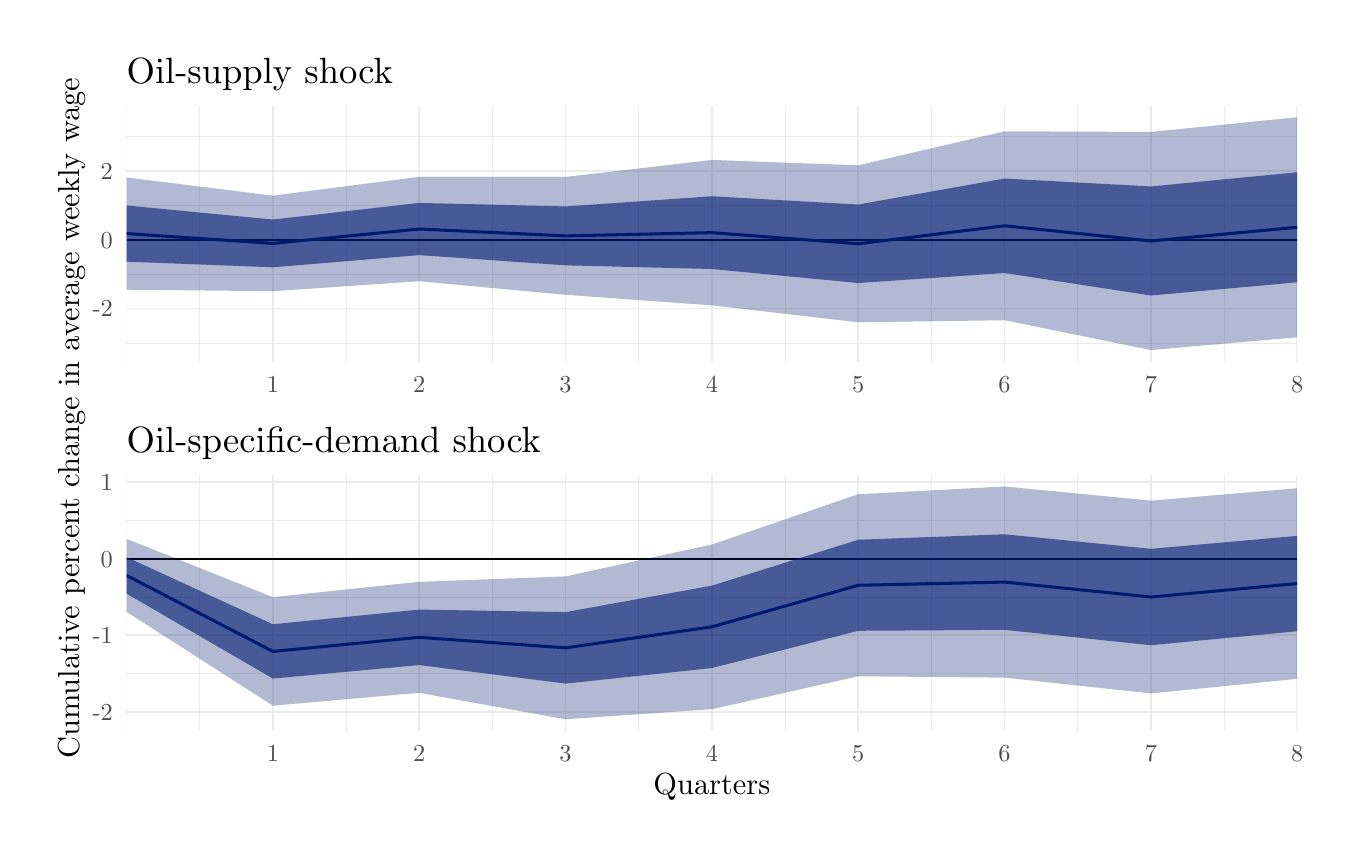
\begin{tikzpicture}[x=1pt,y=1pt]
\definecolor{fillColor}{RGB}{255,255,255}
\path[use as bounding box,fill=fillColor,fill opacity=0.00] (0,0) rectangle (469.75,290.32);
\begin{scope}
\path[clip] (  0.00,  0.00) rectangle (469.75,290.32);
\definecolor{drawColor}{RGB}{255,255,255}
\definecolor{fillColor}{RGB}{255,255,255}

\path[draw=drawColor,line width= 0.6pt,line join=round,line cap=round,fill=fillColor] (  0.00,  0.00) rectangle (469.76,290.32);
\end{scope}
\begin{scope}
\path[clip] ( 35.75,169.62) rectangle (458.75,262.17);
\definecolor{drawColor}{gray}{0.92}

\path[draw=drawColor,line width= 0.3pt,line join=round] ( 35.75,176.38) --
	(458.75,176.38);

\path[draw=drawColor,line width= 0.3pt,line join=round] ( 35.75,201.24) --
	(458.75,201.24);

\path[draw=drawColor,line width= 0.3pt,line join=round] ( 35.75,226.10) --
	(458.75,226.10);

\path[draw=drawColor,line width= 0.3pt,line join=round] ( 35.75,250.96) --
	(458.75,250.96);

\path[draw=drawColor,line width= 0.3pt,line join=round] ( 35.75,169.62) --
	( 35.75,262.17);

\path[draw=drawColor,line width= 0.3pt,line join=round] ( 62.18,169.62) --
	( 62.18,262.17);

\path[draw=drawColor,line width= 0.3pt,line join=round] (115.06,169.62) --
	(115.06,262.17);

\path[draw=drawColor,line width= 0.3pt,line join=round] (167.94,169.62) --
	(167.94,262.17);

\path[draw=drawColor,line width= 0.3pt,line join=round] (220.81,169.62) --
	(220.81,262.17);

\path[draw=drawColor,line width= 0.3pt,line join=round] (273.69,169.62) --
	(273.69,262.17);

\path[draw=drawColor,line width= 0.3pt,line join=round] (326.56,169.62) --
	(326.56,262.17);

\path[draw=drawColor,line width= 0.3pt,line join=round] (379.44,169.62) --
	(379.44,262.17);

\path[draw=drawColor,line width= 0.3pt,line join=round] (432.32,169.62) --
	(432.32,262.17);

\path[draw=drawColor,line width= 0.6pt,line join=round] ( 35.75,188.81) --
	(458.75,188.81);

\path[draw=drawColor,line width= 0.6pt,line join=round] ( 35.75,213.67) --
	(458.75,213.67);

\path[draw=drawColor,line width= 0.6pt,line join=round] ( 35.75,238.53) --
	(458.75,238.53);

\path[draw=drawColor,line width= 0.6pt,line join=round] ( 88.62,169.62) --
	( 88.62,262.17);

\path[draw=drawColor,line width= 0.6pt,line join=round] (141.50,169.62) --
	(141.50,262.17);

\path[draw=drawColor,line width= 0.6pt,line join=round] (194.37,169.62) --
	(194.37,262.17);

\path[draw=drawColor,line width= 0.6pt,line join=round] (247.25,169.62) --
	(247.25,262.17);

\path[draw=drawColor,line width= 0.6pt,line join=round] (300.13,169.62) --
	(300.13,262.17);

\path[draw=drawColor,line width= 0.6pt,line join=round] (353.00,169.62) --
	(353.00,262.17);

\path[draw=drawColor,line width= 0.6pt,line join=round] (405.88,169.62) --
	(405.88,262.17);

\path[draw=drawColor,line width= 0.6pt,line join=round] (458.75,169.62) --
	(458.75,262.17);
\definecolor{drawColor}{RGB}{0,0,0}

\path[draw=drawColor,line width= 0.6pt,line join=round] ( 35.75,213.67) -- (458.75,213.67);
\definecolor{drawColor}{RGB}{0,26,112}

\path[draw=drawColor,line width= 1.1pt,line join=round] ( 35.75,215.91) --
	( 88.62,212.36) --
	(141.50,217.56) --
	(194.37,215.08) --
	(247.25,216.25) --
	(300.13,212.23) --
	(353.00,218.73) --
	(405.88,213.23) --
	(458.75,218.20);
\definecolor{fillColor}{RGB}{0,26,112}

\path[fill=fillColor,fill opacity=0.60] ( 35.75,226.06) --
	( 88.62,220.99) --
	(141.50,226.99) --
	(194.37,225.72) --
	(247.25,229.39) --
	(300.13,226.41) --
	(353.00,235.80) --
	(405.88,232.94) --
	(458.75,238.08) --
	(458.75,198.32) --
	(405.88,193.53) --
	(353.00,201.67) --
	(300.13,198.05) --
	(247.25,203.11) --
	(194.37,204.44) --
	(141.50,208.13) --
	( 88.62,203.73) --
	( 35.75,205.77) --
	cycle;

\path[] ( 35.75,226.06) --
	( 88.62,220.99) --
	(141.50,226.99) --
	(194.37,225.72) --
	(247.25,229.39) --
	(300.13,226.41) --
	(353.00,235.80) --
	(405.88,232.94) --
	(458.75,238.08);

\path[] (458.75,198.32) --
	(405.88,193.53) --
	(353.00,201.67) --
	(300.13,198.05) --
	(247.25,203.11) --
	(194.37,204.44) --
	(141.50,208.13) --
	( 88.62,203.73) --
	( 35.75,205.77);
\definecolor{fillColor}{RGB}{0,26,112}

\path[fill=fillColor,fill opacity=0.30] ( 35.75,236.20) --
	( 88.62,229.62) --
	(141.50,236.42) --
	(194.37,236.37) --
	(247.25,242.53) --
	(300.13,240.58) --
	(353.00,252.87) --
	(405.88,252.64) --
	(458.75,257.96) --
	(458.75,178.44) --
	(405.88,173.82) --
	(353.00,184.60) --
	(300.13,183.87) --
	(247.25,189.97) --
	(194.37,193.79) --
	(141.50,198.69) --
	( 88.62,195.10) --
	( 35.75,195.63) --
	cycle;

\path[] ( 35.75,236.20) --
	( 88.62,229.62) --
	(141.50,236.42) --
	(194.37,236.37) --
	(247.25,242.53) --
	(300.13,240.58) --
	(353.00,252.87) --
	(405.88,252.64) --
	(458.75,257.96);

\path[] (458.75,178.44) --
	(405.88,173.82) --
	(353.00,184.60) --
	(300.13,183.87) --
	(247.25,189.97) --
	(194.37,193.79) --
	(141.50,198.69) --
	( 88.62,195.10) --
	( 35.75,195.63);
\end{scope}
\begin{scope}
\path[clip] (  0.00,  0.00) rectangle (469.75,290.32);
\definecolor{drawColor}{gray}{0.30}

\node[text=drawColor,anchor=base east,inner sep=0pt, outer sep=0pt, scale=  0.88] at ( 30.80,185.78) {-2};

\node[text=drawColor,anchor=base east,inner sep=0pt, outer sep=0pt, scale=  0.88] at ( 30.80,210.64) {0};

\node[text=drawColor,anchor=base east,inner sep=0pt, outer sep=0pt, scale=  0.88] at ( 30.80,235.50) {2};
\end{scope}
\begin{scope}
\path[clip] (  0.00,  0.00) rectangle (469.75,290.32);
\definecolor{drawColor}{gray}{0.30}

\node[text=drawColor,anchor=base,inner sep=0pt, outer sep=0pt, scale=  0.88] at ( 88.62,158.61) {1};

\node[text=drawColor,anchor=base,inner sep=0pt, outer sep=0pt, scale=  0.88] at (141.50,158.61) {2};

\node[text=drawColor,anchor=base,inner sep=0pt, outer sep=0pt, scale=  0.88] at (194.37,158.61) {3};

\node[text=drawColor,anchor=base,inner sep=0pt, outer sep=0pt, scale=  0.88] at (247.25,158.61) {4};

\node[text=drawColor,anchor=base,inner sep=0pt, outer sep=0pt, scale=  0.88] at (300.13,158.61) {5};

\node[text=drawColor,anchor=base,inner sep=0pt, outer sep=0pt, scale=  0.88] at (353.00,158.61) {6};

\node[text=drawColor,anchor=base,inner sep=0pt, outer sep=0pt, scale=  0.88] at (405.88,158.61) {7};

\node[text=drawColor,anchor=base,inner sep=0pt, outer sep=0pt, scale=  0.88] at (458.75,158.61) {8};
\end{scope}
\begin{scope}
\path[clip] (  0.00,  0.00) rectangle (469.75,290.32);
\definecolor{drawColor}{RGB}{0,0,0}

\node[text=drawColor,anchor=base west,inner sep=0pt, outer sep=0pt, scale=  1.32] at ( 35.75,270.23) {Oil-supply shock};
\end{scope}
\begin{scope}
\path[clip] ( 35.75, 36.19) rectangle (458.75,128.74);
\definecolor{drawColor}{gray}{0.92}

\path[draw=drawColor,line width= 0.3pt,line join=round] ( 35.75, 56.95) --
	(458.75, 56.95);

\path[draw=drawColor,line width= 0.3pt,line join=round] ( 35.75, 84.60) --
	(458.75, 84.60);

\path[draw=drawColor,line width= 0.3pt,line join=round] ( 35.75,112.25) --
	(458.75,112.25);

\path[draw=drawColor,line width= 0.3pt,line join=round] ( 35.75, 36.19) --
	( 35.75,128.74);

\path[draw=drawColor,line width= 0.3pt,line join=round] ( 62.18, 36.19) --
	( 62.18,128.74);

\path[draw=drawColor,line width= 0.3pt,line join=round] (115.06, 36.19) --
	(115.06,128.74);

\path[draw=drawColor,line width= 0.3pt,line join=round] (167.94, 36.19) --
	(167.94,128.74);

\path[draw=drawColor,line width= 0.3pt,line join=round] (220.81, 36.19) --
	(220.81,128.74);

\path[draw=drawColor,line width= 0.3pt,line join=round] (273.69, 36.19) --
	(273.69,128.74);

\path[draw=drawColor,line width= 0.3pt,line join=round] (326.56, 36.19) --
	(326.56,128.74);

\path[draw=drawColor,line width= 0.3pt,line join=round] (379.44, 36.19) --
	(379.44,128.74);

\path[draw=drawColor,line width= 0.3pt,line join=round] (432.32, 36.19) --
	(432.32,128.74);

\path[draw=drawColor,line width= 0.6pt,line join=round] ( 35.75, 43.13) --
	(458.75, 43.13);

\path[draw=drawColor,line width= 0.6pt,line join=round] ( 35.75, 70.78) --
	(458.75, 70.78);

\path[draw=drawColor,line width= 0.6pt,line join=round] ( 35.75, 98.43) --
	(458.75, 98.43);

\path[draw=drawColor,line width= 0.6pt,line join=round] ( 35.75,126.07) --
	(458.75,126.07);

\path[draw=drawColor,line width= 0.6pt,line join=round] ( 88.62, 36.19) --
	( 88.62,128.74);

\path[draw=drawColor,line width= 0.6pt,line join=round] (141.50, 36.19) --
	(141.50,128.74);

\path[draw=drawColor,line width= 0.6pt,line join=round] (194.37, 36.19) --
	(194.37,128.74);

\path[draw=drawColor,line width= 0.6pt,line join=round] (247.25, 36.19) --
	(247.25,128.74);

\path[draw=drawColor,line width= 0.6pt,line join=round] (300.13, 36.19) --
	(300.13,128.74);

\path[draw=drawColor,line width= 0.6pt,line join=round] (353.00, 36.19) --
	(353.00,128.74);

\path[draw=drawColor,line width= 0.6pt,line join=round] (405.88, 36.19) --
	(405.88,128.74);

\path[draw=drawColor,line width= 0.6pt,line join=round] (458.75, 36.19) --
	(458.75,128.74);
\definecolor{drawColor}{RGB}{0,0,0}

\path[draw=drawColor,line width= 0.6pt,line join=round] ( 35.75, 98.43) -- (458.75, 98.43);
\definecolor{drawColor}{RGB}{0,26,112}

\path[draw=drawColor,line width= 1.1pt,line join=round] ( 35.75, 92.39) --
	( 88.62, 64.93) --
	(141.50, 70.02) --
	(194.37, 66.22) --
	(247.25, 73.81) --
	(300.13, 88.83) --
	(353.00, 89.99) --
	(405.88, 84.59) --
	(458.75, 89.45);
\definecolor{fillColor}{RGB}{0,26,112}

\path[fill=fillColor,fill opacity=0.60] ( 35.75, 98.99) --
	( 88.62, 74.73) --
	(141.50, 80.05) --
	(194.37, 79.13) --
	(247.25, 88.69) --
	(300.13,105.28) --
	(353.00,107.26) --
	(405.88,102.00) --
	(458.75,106.67) --
	(458.75, 72.23) --
	(405.88, 67.17) --
	(353.00, 72.72) --
	(300.13, 72.38) --
	(247.25, 58.93) --
	(194.37, 53.31) --
	(141.50, 60.00) --
	( 88.62, 55.12) --
	( 35.75, 85.80) --
	cycle;

\path[] ( 35.75, 98.99) --
	( 88.62, 74.73) --
	(141.50, 80.05) --
	(194.37, 79.13) --
	(247.25, 88.69) --
	(300.13,105.28) --
	(353.00,107.26) --
	(405.88,102.00) --
	(458.75,106.67);

\path[] (458.75, 72.23) --
	(405.88, 67.17) --
	(353.00, 72.72) --
	(300.13, 72.38) --
	(247.25, 58.93) --
	(194.37, 53.31) --
	(141.50, 60.00) --
	( 88.62, 55.12) --
	( 35.75, 85.80);
\definecolor{fillColor}{RGB}{0,26,112}

\path[fill=fillColor,fill opacity=0.30] ( 35.75,105.58) --
	( 88.62, 84.54) --
	(141.50, 90.08) --
	(194.37, 92.04) --
	(247.25,103.56) --
	(300.13,121.73) --
	(353.00,124.53) --
	(405.88,119.41) --
	(458.75,123.89) --
	(458.75, 55.01) --
	(405.88, 49.76) --
	(353.00, 55.45) --
	(300.13, 55.94) --
	(247.25, 44.06) --
	(194.37, 40.39) --
	(141.50, 49.97) --
	( 88.62, 45.32) --
	( 35.75, 79.20) --
	cycle;

\path[] ( 35.75,105.58) --
	( 88.62, 84.54) --
	(141.50, 90.08) --
	(194.37, 92.04) --
	(247.25,103.56) --
	(300.13,121.73) --
	(353.00,124.53) --
	(405.88,119.41) --
	(458.75,123.89);

\path[] (458.75, 55.01) --
	(405.88, 49.76) --
	(353.00, 55.45) --
	(300.13, 55.94) --
	(247.25, 44.06) --
	(194.37, 40.39) --
	(141.50, 49.97) --
	( 88.62, 45.32) --
	( 35.75, 79.20);
\end{scope}
\begin{scope}
\path[clip] (  0.00,  0.00) rectangle (469.75,290.32);
\definecolor{drawColor}{gray}{0.30}

\node[text=drawColor,anchor=base east,inner sep=0pt, outer sep=0pt, scale=  0.88] at ( 30.80, 40.10) {-2};

\node[text=drawColor,anchor=base east,inner sep=0pt, outer sep=0pt, scale=  0.88] at ( 30.80, 67.75) {-1};

\node[text=drawColor,anchor=base east,inner sep=0pt, outer sep=0pt, scale=  0.88] at ( 30.80, 95.40) {0};

\node[text=drawColor,anchor=base east,inner sep=0pt, outer sep=0pt, scale=  0.88] at ( 30.80,123.04) {1};
\end{scope}
\begin{scope}
\path[clip] (  0.00,  0.00) rectangle (469.75,290.32);
\definecolor{drawColor}{gray}{0.30}

\node[text=drawColor,anchor=base,inner sep=0pt, outer sep=0pt, scale=  0.88] at ( 88.62, 25.18) {1};

\node[text=drawColor,anchor=base,inner sep=0pt, outer sep=0pt, scale=  0.88] at (141.50, 25.18) {2};

\node[text=drawColor,anchor=base,inner sep=0pt, outer sep=0pt, scale=  0.88] at (194.37, 25.18) {3};

\node[text=drawColor,anchor=base,inner sep=0pt, outer sep=0pt, scale=  0.88] at (247.25, 25.18) {4};

\node[text=drawColor,anchor=base,inner sep=0pt, outer sep=0pt, scale=  0.88] at (300.13, 25.18) {5};

\node[text=drawColor,anchor=base,inner sep=0pt, outer sep=0pt, scale=  0.88] at (353.00, 25.18) {6};

\node[text=drawColor,anchor=base,inner sep=0pt, outer sep=0pt, scale=  0.88] at (405.88, 25.18) {7};

\node[text=drawColor,anchor=base,inner sep=0pt, outer sep=0pt, scale=  0.88] at (458.75, 25.18) {8};
\end{scope}
\begin{scope}
\path[clip] (  0.00,  0.00) rectangle (469.75,290.32);
\definecolor{drawColor}{RGB}{0,0,0}

\node[text=drawColor,anchor=base,inner sep=0pt, outer sep=0pt, scale=  1.10] at (247.25, 13.14) {Quarters};
\end{scope}
\begin{scope}
\path[clip] (  0.00,  0.00) rectangle (469.75,290.32);
\definecolor{drawColor}{RGB}{0,0,0}

\node[text=drawColor,rotate= 90.00,anchor=base,inner sep=0pt, outer sep=0pt, scale=  1.10] at ( 18.58,149.18) {Cumulative percent change in average weekly wage};
\end{scope}
\begin{scope}
\path[clip] (  0.00,  0.00) rectangle (469.75,290.32);
\definecolor{drawColor}{RGB}{0,0,0}

\node[text=drawColor,anchor=base west,inner sep=0pt, outer sep=0pt, scale=  1.32] at ( 35.75,136.80) {Oil-specific-demand shock};
\end{scope}
\end{tikzpicture}

  }
  \caption[]{\label{fig:wage-oil-supply-shock} Responses of the average real wage to
    oil-supply and oil-specific-demand shocks}
\end{figure}

\begin{figure}[htbp]
  \centering
  % \resizebox{<horizontal size>}{<vertical size>}{%
  \resizebox{\textwidth}{!}{
  % Created by tikzDevice version 0.12.6 on 2026-05-29 10:59:11
% !TEX encoding = UTF-8 Unicode
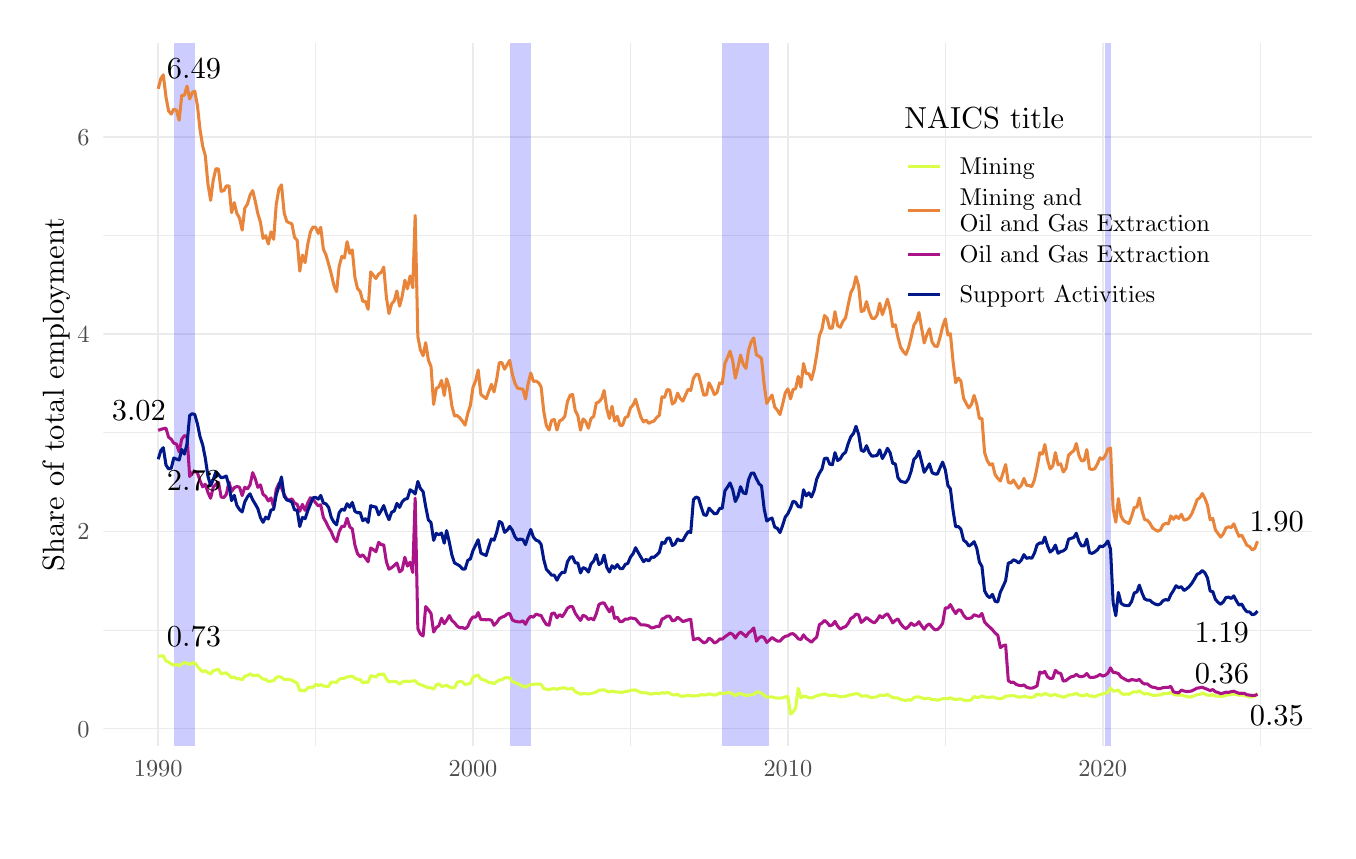
\begin{tikzpicture}[x=1pt,y=1pt]
\definecolor{fillColor}{RGB}{255,255,255}
\path[use as bounding box,fill=fillColor,fill opacity=0.00] (0,0) rectangle (469.75,290.32);
\begin{scope}
\path[clip] (  0.00,  0.00) rectangle (469.75,290.32);
\definecolor{fillColor}{RGB}{255,255,255}

\path[fill=fillColor] (  0.00,  0.00) rectangle (469.76,290.32);
\end{scope}
\begin{scope}
\path[clip] ( 27.31, 30.69) rectangle (464.25,284.82);
\definecolor{drawColor}{gray}{0.92}

\path[draw=drawColor,line width= 0.3pt,line join=round] ( 27.31, 72.66) --
	(464.25, 72.66);

\path[draw=drawColor,line width= 0.3pt,line join=round] ( 27.31,143.93) --
	(464.25,143.93);

\path[draw=drawColor,line width= 0.3pt,line join=round] ( 27.31,215.20) --
	(464.25,215.20);

\path[draw=drawColor,line width= 0.3pt,line join=round] (104.05, 30.69) --
	(104.05,284.82);

\path[draw=drawColor,line width= 0.3pt,line join=round] (217.81, 30.69) --
	(217.81,284.82);

\path[draw=drawColor,line width= 0.3pt,line join=round] (331.58, 30.69) --
	(331.58,284.82);

\path[draw=drawColor,line width= 0.3pt,line join=round] (445.33, 30.69) --
	(445.33,284.82);

\path[draw=drawColor,line width= 0.6pt,line join=round] ( 27.31, 37.02) --
	(464.25, 37.02);

\path[draw=drawColor,line width= 0.6pt,line join=round] ( 27.31,108.29) --
	(464.25,108.29);

\path[draw=drawColor,line width= 0.6pt,line join=round] ( 27.31,179.56) --
	(464.25,179.56);

\path[draw=drawColor,line width= 0.6pt,line join=round] ( 27.31,250.83) --
	(464.25,250.83);

\path[draw=drawColor,line width= 0.6pt,line join=round] ( 47.17, 30.69) --
	( 47.17,284.82);

\path[draw=drawColor,line width= 0.6pt,line join=round] (160.92, 30.69) --
	(160.92,284.82);

\path[draw=drawColor,line width= 0.6pt,line join=round] (274.70, 30.69) --
	(274.70,284.82);

\path[draw=drawColor,line width= 0.6pt,line join=round] (388.45, 30.69) --
	(388.45,284.82);
\definecolor{fillColor}{RGB}{0,0,255}

\path[fill=fillColor,fill opacity=0.20] ( 52.81, 30.69) rectangle ( 60.38,284.82);

\path[fill=fillColor,fill opacity=0.20] (174.16, 30.69) rectangle (181.79,284.82);

\path[fill=fillColor,fill opacity=0.20] (250.97, 30.69) rectangle (268.04,284.82);

\path[fill=fillColor,fill opacity=0.20] (389.42, 30.69) rectangle (391.29,284.82);
\definecolor{drawColor}{RGB}{218,255,71}

\path[draw=drawColor,line width= 1.1pt,line join=round] ( 47.17, 63.11) --
	( 48.14, 63.29) --
	( 49.01, 63.36) --
	( 49.98, 61.46) --
	( 50.91, 61.05) --
	( 51.88, 60.41) --
	( 52.81, 59.94) --
	( 53.78, 60.17) --
	( 54.74, 59.80) --
	( 55.68, 60.39) --
	( 56.64, 60.78) --
	( 57.58, 60.74) --
	( 58.54, 60.23) --
	( 59.51, 60.65) --
	( 60.38, 60.85) --
	( 61.35, 59.51) --
	( 62.28, 58.46) --
	( 63.25, 57.58) --
	( 64.18, 58.01) --
	( 65.15, 57.25) --
	( 66.11, 56.85) --
	( 67.05, 57.94) --
	( 68.01, 58.25) --
	( 68.95, 58.46) --
	( 69.91, 56.85) --
	( 70.88, 57.05) --
	( 71.78, 57.18) --
	( 72.75, 56.35) --
	( 73.68, 55.42) --
	( 74.65, 55.69) --
	( 75.58, 55.03) --
	( 76.55, 55.07) --
	( 77.51, 54.63) --
	( 78.45, 55.99) --
	( 79.41, 56.18) --
	( 80.35, 56.86) --
	( 81.31, 56.23) --
	( 82.28, 56.16) --
	( 83.15, 56.45) --
	( 84.11, 55.66) --
	( 85.05, 54.96) --
	( 86.01, 54.79) --
	( 86.95, 54.09) --
	( 87.91, 54.18) --
	( 88.88, 54.43) --
	( 89.81, 55.48) --
	( 90.78, 55.84) --
	( 91.71, 55.58) --
	( 92.68, 54.76) --
	( 93.65, 54.79) --
	( 94.52, 54.83) --
	( 95.48, 54.53) --
	( 96.42, 53.93) --
	( 97.38, 53.53) --
	( 98.32, 50.74) --
	( 99.28, 50.83) --
	(100.25, 50.66) --
	(101.18, 51.76) --
	(102.15, 52.02) --
	(103.08, 51.93) --
	(104.05, 53.02) --
	(105.01, 52.56) --
	(105.89, 52.98) --
	(106.85, 52.44) --
	(107.79, 52.31) --
	(108.75, 52.29) --
	(109.69, 53.86) --
	(110.65, 53.86) --
	(111.62, 53.69) --
	(112.55, 54.86) --
	(113.52, 55.21) --
	(114.45, 55.20) --
	(115.42, 55.70) --
	(116.38, 55.86) --
	(117.29, 56.02) --
	(118.25, 55.25) --
	(119.19, 54.85) --
	(120.15, 54.82) --
	(121.09, 53.52) --
	(122.05, 53.91) --
	(123.02, 53.70) --
	(123.95, 56.19) --
	(124.92, 55.95) --
	(125.85, 55.65) --
	(126.82, 56.72) --
	(127.78, 56.59) --
	(128.66, 56.80) --
	(129.62, 54.97) --
	(130.56, 53.88) --
	(131.52, 54.14) --
	(132.46, 54.03) --
	(133.42, 53.93) --
	(134.39, 53.09) --
	(135.32, 53.84) --
	(136.29, 54.20) --
	(137.22, 54.09) --
	(138.19, 54.13) --
	(139.15, 54.23) --
	(140.02, 54.37) --
	(140.99, 53.28) --
	(141.92, 52.93) --
	(142.89, 52.62) --
	(143.82, 52.13) --
	(144.79, 51.83) --
	(145.76, 51.77) --
	(146.69, 51.25) --
	(147.66, 52.87) --
	(148.59, 53.23) --
	(149.55, 52.31) --
	(150.52, 52.43) --
	(151.39, 52.74) --
	(152.36, 52.07) --
	(153.29, 51.77) --
	(154.26, 51.88) --
	(155.19, 53.73) --
	(156.16, 54.11) --
	(157.12, 53.90) --
	(158.06, 52.95) --
	(159.02, 53.16) --
	(159.96, 53.36) --
	(160.92, 55.65) --
	(161.89, 56.13) --
	(162.79, 56.40) --
	(163.76, 54.93) --
	(164.69, 54.65) --
	(165.66, 54.34) --
	(166.59, 53.70) --
	(167.56, 53.69) --
	(168.52, 53.22) --
	(169.46, 53.96) --
	(170.42, 54.64) --
	(171.36, 54.69) --
	(172.32, 55.34) --
	(173.29, 55.44) --
	(174.16, 55.39) --
	(175.13, 54.08) --
	(176.06, 53.66) --
	(177.03, 53.26) --
	(177.96, 52.83) --
	(178.93, 52.38) --
	(179.89, 51.94) --
	(180.83, 52.57) --
	(181.79, 52.97) --
	(182.73, 53.02) --
	(183.69, 53.13) --
	(184.66, 53.15) --
	(185.53, 53.03) --
	(186.50, 51.50) --
	(187.43, 51.29) --
	(188.40, 51.07) --
	(189.33, 51.41) --
	(190.30, 51.51) --
	(191.26, 51.23) --
	(192.20, 51.58) --
	(193.16, 51.74) --
	(194.10, 51.73) --
	(195.06, 51.38) --
	(196.03, 51.44) --
	(196.90, 51.57) --
	(197.86, 50.37) --
	(198.80, 49.98) --
	(199.76, 49.49) --
	(200.70, 49.74) --
	(201.66, 49.64) --
	(202.63, 49.55) --
	(203.56, 49.69) --
	(204.53, 50.00) --
	(205.46, 50.26) --
	(206.43, 50.95) --
	(207.40, 50.94) --
	(208.30, 51.08) --
	(209.26, 50.56) --
	(210.20, 50.28) --
	(211.16, 50.61) --
	(212.10, 50.34) --
	(213.06, 50.33) --
	(214.03, 50.12) --
	(214.96, 50.12) --
	(215.93, 50.51) --
	(216.86, 50.51) --
	(217.83, 50.91) --
	(218.80, 50.92) --
	(219.67, 51.02) --
	(220.63, 50.51) --
	(221.57, 50.11) --
	(222.53, 50.00) --
	(223.47, 49.94) --
	(224.43, 49.67) --
	(225.40, 49.50) --
	(226.33, 49.74) --
	(227.30, 49.75) --
	(228.23, 49.66) --
	(229.20, 50.03) --
	(230.16, 49.81) --
	(231.04, 50.07) --
	(232.00, 49.88) --
	(232.94, 49.20) --
	(233.90, 49.21) --
	(234.84, 49.45) --
	(235.80, 48.84) --
	(236.77, 48.68) --
	(237.70, 48.87) --
	(238.67, 49.10) --
	(239.60, 48.91) --
	(240.57, 48.79) --
	(241.53, 48.94) --
	(242.40, 48.94) --
	(243.37, 49.34) --
	(244.30, 49.18) --
	(245.27, 49.23) --
	(246.20, 49.57) --
	(247.17, 49.37) --
	(248.14, 49.14) --
	(249.07, 49.30) --
	(250.04, 49.98) --
	(250.97, 49.70) --
	(251.94, 49.85) --
	(252.90, 49.94) --
	(253.80, 50.09) --
	(254.77, 49.53) --
	(255.70, 48.90) --
	(256.67, 49.55) --
	(257.60, 49.70) --
	(258.57, 49.31) --
	(259.54, 49.01) --
	(260.47, 49.14) --
	(261.44, 49.22) --
	(262.37, 49.41) --
	(263.34, 50.19) --
	(264.30, 50.30) --
	(265.17, 49.79) --
	(266.14, 49.01) --
	(267.07, 48.39) --
	(268.04, 48.48) --
	(268.97, 48.50) --
	(269.94, 48.18) --
	(270.90, 48.05) --
	(271.84, 48.08) --
	(272.80, 48.16) --
	(273.74, 48.51) --
	(274.70, 48.60) --
	(275.67, 42.24) --
	(276.54, 43.03) --
	(277.51, 44.53) --
	(278.44, 51.57) --
	(279.41, 48.17) --
	(280.34, 48.75) --
	(281.31, 48.60) --
	(282.27, 48.17) --
	(283.21, 48.14) --
	(284.17, 48.45) --
	(285.11, 48.90) --
	(286.07, 49.12) --
	(287.04, 49.39) --
	(287.91, 49.58) --
	(288.88, 49.27) --
	(289.81, 48.94) --
	(290.78, 48.92) --
	(291.71, 49.18) --
	(292.68, 48.78) --
	(293.64, 48.53) --
	(294.58, 48.57) --
	(295.54, 48.68) --
	(296.48, 49.08) --
	(297.44, 49.22) --
	(298.41, 49.44) --
	(299.31, 49.67) --
	(300.28, 49.54) --
	(301.21, 48.82) --
	(302.18, 48.80) --
	(303.11, 48.94) --
	(304.08, 48.50) --
	(305.04, 48.21) --
	(305.98, 48.39) --
	(306.94, 48.51) --
	(307.88, 49.17) --
	(308.84, 49.01) --
	(309.81, 49.09) --
	(310.68, 49.38) --
	(311.64, 48.79) --
	(312.58, 48.22) --
	(313.54, 48.16) --
	(314.48, 48.12) --
	(315.44, 47.51) --
	(316.41, 47.37) --
	(317.34, 47.16) --
	(318.31, 47.49) --
	(319.24, 47.27) --
	(320.21, 48.22) --
	(321.18, 48.50) --
	(322.05, 48.47) --
	(323.01, 48.16) --
	(323.95, 47.83) --
	(324.91, 47.94) --
	(325.85, 47.98) --
	(326.81, 47.52) --
	(327.78, 47.52) --
	(328.71, 47.29) --
	(329.68, 47.48) --
	(330.61, 47.89) --
	(331.58, 47.92) --
	(332.54, 47.83) --
	(333.42, 48.21) --
	(334.38, 47.75) --
	(335.32, 47.50) --
	(336.28, 47.69) --
	(337.22, 47.80) --
	(338.18, 47.33) --
	(339.15, 47.25) --
	(340.08, 47.15) --
	(341.05, 47.56) --
	(341.98, 48.68) --
	(342.95, 48.26) --
	(343.91, 48.35) --
	(344.82, 48.87) --
	(345.78, 48.48) --
	(346.72, 48.33) --
	(347.68, 48.31) --
	(348.62, 48.52) --
	(349.58, 48.20) --
	(350.55, 47.92) --
	(351.48, 47.85) --
	(352.45, 48.13) --
	(353.38, 48.72) --
	(354.35, 48.84) --
	(355.31, 48.92) --
	(356.19, 49.02) --
	(357.15, 48.65) --
	(358.09, 48.39) --
	(359.05, 48.47) --
	(359.99, 48.74) --
	(360.95, 48.49) --
	(361.92, 48.38) --
	(362.85, 48.32) --
	(363.82, 48.60) --
	(364.75, 49.55) --
	(365.72, 49.19) --
	(366.68, 49.16) --
	(367.55, 49.78) --
	(368.52, 49.38) --
	(369.45, 48.94) --
	(370.42, 49.15) --
	(371.35, 49.35) --
	(372.32, 48.89) --
	(373.29, 48.77) --
	(374.22, 48.34) --
	(375.19, 48.67) --
	(376.12, 49.23) --
	(377.08, 49.21) --
	(378.05, 49.45) --
	(378.92, 49.83) --
	(379.89, 49.16) --
	(380.82, 48.96) --
	(381.79, 48.89) --
	(382.72, 49.48) --
	(383.69, 48.76) --
	(384.65, 48.86) --
	(385.59, 48.48) --
	(386.55, 49.04) --
	(387.49, 49.32) --
	(388.45, 49.57) --
	(389.42, 49.82) --
	(390.32, 50.17) --
	(391.29, 51.67) --
	(392.22, 50.62) --
	(393.19, 50.65) --
	(394.12, 50.99) --
	(395.09, 49.83) --
	(396.05, 49.39) --
	(396.99, 49.55) --
	(397.95, 49.43) --
	(398.89, 49.99) --
	(399.85, 50.37) --
	(400.82, 50.25) --
	(401.69, 50.72) --
	(402.66, 50.02) --
	(403.59, 49.54) --
	(404.56, 49.69) --
	(405.49, 49.45) --
	(406.46, 49.06) --
	(407.42, 49.01) --
	(408.36, 49.16) --
	(409.32, 49.21) --
	(410.26, 49.61) --
	(411.22, 49.69) --
	(412.19, 49.66) --
	(413.06, 50.17) --
	(414.03, 49.47) --
	(414.96, 49.18) --
	(415.93, 49.09) --
	(416.86, 49.24) --
	(417.83, 48.88) --
	(418.79, 48.62) --
	(419.73, 48.43) --
	(420.69, 48.57) --
	(421.63, 48.87) --
	(422.59, 49.33) --
	(423.56, 49.46) --
	(424.43, 49.90) --
	(425.39, 49.46) --
	(426.33, 49.11) --
	(427.29, 49.03) --
	(428.23, 49.33) --
	(429.19, 48.77) --
	(430.16, 48.80) --
	(431.09, 48.64) --
	(432.06, 48.72) --
	(432.99, 49.00) --
	(433.96, 49.32) --
	(434.93, 49.27) --
	(435.83, 49.55) --
	(436.79, 49.35) --
	(437.73, 49.08) --
	(438.69, 49.14) --
	(439.63, 49.08) --
	(440.59, 48.77) --
	(441.56, 48.53) --
	(442.49, 48.46) --
	(443.46, 48.78) --
	(444.39, 49.80);
\definecolor{drawColor}{RGB}{232,133,58}

\path[draw=drawColor,line width= 1.1pt,line join=round] ( 47.17,268.24) --
	( 48.14,271.97) --
	( 49.01,273.27) --
	( 49.98,265.27) --
	( 50.91,260.25) --
	( 51.88,259.08) --
	( 52.81,260.92) --
	( 53.78,260.43) --
	( 54.74,256.86) --
	( 55.68,265.87) --
	( 56.64,265.89) --
	( 57.58,269.18) --
	( 58.54,264.56) --
	( 59.51,266.95) --
	( 60.38,267.36) --
	( 61.35,262.06) --
	( 62.28,253.52) --
	( 63.25,247.45) --
	( 64.18,244.09) --
	( 65.15,233.75) --
	( 66.11,227.93) --
	( 67.05,235.21) --
	( 68.01,239.34) --
	( 68.95,239.27) --
	( 69.91,231.20) --
	( 70.88,231.42) --
	( 71.78,233.12) --
	( 72.75,233.14) --
	( 73.68,223.47) --
	( 74.65,227.09) --
	( 75.58,223.22) --
	( 76.55,221.49) --
	( 77.51,217.14) --
	( 78.45,225.12) --
	( 79.41,226.57) --
	( 80.35,229.82) --
	( 81.31,231.43) --
	( 82.28,227.42) --
	( 83.15,223.20) --
	( 84.11,220.03) --
	( 85.05,214.17) --
	( 86.01,215.17) --
	( 86.95,212.15) --
	( 87.91,216.55) --
	( 88.88,213.84) --
	( 89.81,226.34) --
	( 90.78,232.04) --
	( 91.71,233.54) --
	( 92.68,223.38) --
	( 93.65,220.25) --
	( 94.52,219.82) --
	( 95.48,219.42) --
	( 96.42,214.55) --
	( 97.38,213.52) --
	( 98.32,202.34) --
	( 99.28,208.16) --
	(100.25,205.41) --
	(101.18,211.89) --
	(102.15,216.46) --
	(103.08,218.27) --
	(104.05,218.21) --
	(105.01,215.96) --
	(105.89,218.21) --
	(106.85,210.28) --
	(107.79,208.20) --
	(108.75,204.88) --
	(109.69,201.38) --
	(110.65,197.24) --
	(111.62,194.90) --
	(112.55,204.04) --
	(113.52,207.68) --
	(114.45,207.12) --
	(115.42,213.00) --
	(116.38,208.76) --
	(117.29,209.99) --
	(118.25,200.08) --
	(119.19,196.06) --
	(120.15,195.00) --
	(121.09,191.44) --
	(122.05,191.39) --
	(123.02,188.53) --
	(123.95,202.06) --
	(124.92,200.83) --
	(125.85,199.68) --
	(126.82,201.32) --
	(127.78,201.91) --
	(128.66,203.81) --
	(129.62,192.88) --
	(130.56,187.01) --
	(131.52,190.52) --
	(132.46,191.65) --
	(133.42,195.19) --
	(134.39,189.71) --
	(135.32,193.18) --
	(136.29,199.06) --
	(137.22,195.96) --
	(138.19,200.60) --
	(139.15,196.35) --
	(140.02,222.46) --
	(140.99,178.69) --
	(141.92,173.85) --
	(142.89,171.77) --
	(143.82,176.50) --
	(144.79,170.24) --
	(145.76,167.81) --
	(146.69,154.19) --
	(147.66,159.98) --
	(148.59,160.50) --
	(149.55,162.88) --
	(150.52,157.39) --
	(151.39,163.45) --
	(152.36,160.32) --
	(153.29,153.55) --
	(154.26,149.97) --
	(155.19,150.18) --
	(156.16,149.31) --
	(157.12,148.12) --
	(158.06,146.70) --
	(159.02,150.86) --
	(159.96,153.81) --
	(160.92,160.36) --
	(161.89,162.79) --
	(162.79,166.64) --
	(163.76,157.78) --
	(164.69,157.04) --
	(165.66,156.24) --
	(166.59,158.74) --
	(167.56,161.44) --
	(168.52,158.69) --
	(169.46,163.14) --
	(170.42,169.28) --
	(171.36,169.28) --
	(172.32,166.90) --
	(173.29,168.58) --
	(174.16,170.11) --
	(175.13,165.10) --
	(176.06,161.83) --
	(177.03,160.05) --
	(177.96,159.86) --
	(178.93,159.70) --
	(179.89,156.13) --
	(180.83,161.62) --
	(181.79,165.54) --
	(182.73,162.51) --
	(183.69,162.61) --
	(184.66,161.97) --
	(185.53,160.53) --
	(186.50,151.57) --
	(187.43,146.50) --
	(188.40,144.94) --
	(189.33,148.45) --
	(190.30,148.74) --
	(191.26,144.93) --
	(192.20,148.21) --
	(193.16,148.71) --
	(194.10,149.92) --
	(195.06,155.23) --
	(196.03,157.50) --
	(196.90,157.77) --
	(197.86,151.98) --
	(198.80,150.16) --
	(199.76,144.88) --
	(200.70,148.95) --
	(201.66,147.94) --
	(202.63,145.58) --
	(203.56,149.08) --
	(204.53,149.88) --
	(205.46,154.65) --
	(206.43,155.11) --
	(207.40,156.33) --
	(208.30,159.21) --
	(209.26,152.63) --
	(210.20,149.10) --
	(211.16,153.48) --
	(212.10,148.14) --
	(213.06,149.89) --
	(214.03,146.64) --
	(214.96,146.65) --
	(215.93,149.46) --
	(216.86,149.78) --
	(217.83,152.94) --
	(218.80,154.03) --
	(219.67,156.06) --
	(220.63,152.61) --
	(221.57,149.61) --
	(222.53,147.86) --
	(223.47,148.51) --
	(224.43,147.36) --
	(225.40,147.85) --
	(226.33,148.20) --
	(227.30,149.48) --
	(228.23,150.25) --
	(229.20,156.91) --
	(230.16,156.73) --
	(231.04,159.52) --
	(232.00,159.38) --
	(232.94,154.33) --
	(233.90,155.11) --
	(234.84,158.25) --
	(235.80,156.31) --
	(236.77,155.37) --
	(237.70,157.56) --
	(238.67,159.65) --
	(239.60,159.24) --
	(240.57,163.65) --
	(241.53,165.05) --
	(242.40,164.96) --
	(243.37,161.25) --
	(244.30,157.52) --
	(245.27,157.64) --
	(246.20,161.99) --
	(247.17,160.12) --
	(248.14,157.72) --
	(249.07,158.45) --
	(250.04,161.95) --
	(250.97,161.68) --
	(251.94,168.97) --
	(252.90,171.11) --
	(253.80,173.43) --
	(254.77,169.89) --
	(255.70,163.65) --
	(256.67,167.67) --
	(257.60,172.02) --
	(258.57,168.66) --
	(259.54,167.17) --
	(260.47,173.63) --
	(261.44,176.85) --
	(262.37,178.19) --
	(263.34,172.06) --
	(264.30,171.55) --
	(265.17,170.79) --
	(266.14,161.21) --
	(267.07,154.54) --
	(268.04,156.20) --
	(268.97,157.57) --
	(269.94,153.23) --
	(270.90,152.07) --
	(271.84,150.53) --
	(272.80,154.26) --
	(273.74,158.29) --
	(274.70,159.84) --
	(275.67,156.18) --
	(276.54,159.51) --
	(277.51,159.91) --
	(278.44,164.30) --
	(279.41,160.41) --
	(280.34,168.96) --
	(281.31,165.34) --
	(282.27,165.34) --
	(283.21,163.10) --
	(284.17,166.72) --
	(285.11,172.12) --
	(286.07,178.96) --
	(287.04,181.44) --
	(287.91,186.31) --
	(288.88,185.38) --
	(289.81,181.68) --
	(290.78,181.79) --
	(291.71,187.70) --
	(292.68,182.67) --
	(293.64,182.05) --
	(294.58,184.18) --
	(295.54,185.44) --
	(296.48,190.07) --
	(297.44,194.54) --
	(298.41,196.46) --
	(299.31,200.34) --
	(300.28,196.95) --
	(301.21,187.76) --
	(302.18,188.13) --
	(303.11,191.34) --
	(304.08,187.67) --
	(305.04,185.33) --
	(305.98,185.18) --
	(306.94,186.51) --
	(307.88,190.74) --
	(308.84,186.64) --
	(309.81,189.35) --
	(310.68,192.20) --
	(311.64,188.47) --
	(312.58,182.31) --
	(313.54,182.95) --
	(314.48,178.43) --
	(315.44,174.85) --
	(316.41,173.27) --
	(317.34,172.24) --
	(318.31,174.70) --
	(319.24,178.43) --
	(320.21,182.78) --
	(321.18,184.41) --
	(322.05,187.40) --
	(323.01,181.77) --
	(323.95,176.38) --
	(324.91,179.33) --
	(325.85,181.52) --
	(326.81,176.73) --
	(327.78,175.26) --
	(328.71,175.11) --
	(329.68,178.45) --
	(330.61,182.27) --
	(331.58,185.10) --
	(332.54,179.24) --
	(333.42,179.75) --
	(334.38,169.70) --
	(335.32,162.02) --
	(336.28,163.69) --
	(337.22,162.61) --
	(338.18,156.39) --
	(339.15,154.50) --
	(340.08,152.94) --
	(341.05,154.22) --
	(341.98,157.42) --
	(342.95,154.26) --
	(343.91,149.08) --
	(344.82,149.15) --
	(345.78,136.79) --
	(346.72,133.89) --
	(347.68,132.27) --
	(348.62,132.77) --
	(349.58,128.78) --
	(350.55,127.46) --
	(351.48,126.50) --
	(352.45,129.45) --
	(353.38,132.45) --
	(354.35,126.05) --
	(355.31,125.68) --
	(356.19,126.85) --
	(357.15,125.30) --
	(358.09,123.92) --
	(359.05,124.90) --
	(359.99,127.43) --
	(360.95,125.00) --
	(361.92,124.83) --
	(362.85,124.51) --
	(363.82,127.03) --
	(364.75,131.46) --
	(365.72,136.76) --
	(366.68,136.25) --
	(367.55,139.69) --
	(368.52,134.12) --
	(369.45,130.87) --
	(370.42,131.95) --
	(371.35,136.77) --
	(372.32,132.41) --
	(373.29,132.73) --
	(374.22,129.76) --
	(375.19,131.09) --
	(376.12,135.80) --
	(377.08,136.75) --
	(378.05,137.51) --
	(378.92,140.06) --
	(379.89,135.70) --
	(380.82,133.76) --
	(381.79,134.00) --
	(382.72,137.87) --
	(383.69,130.92) --
	(384.65,130.67) --
	(385.59,130.95) --
	(386.55,132.67) --
	(387.49,134.90) --
	(388.45,134.29) --
	(389.42,135.72) --
	(390.32,137.98) --
	(391.29,138.46) --
	(392.22,116.51) --
	(393.19,111.65) --
	(394.12,120.14) --
	(395.09,113.77) --
	(396.05,112.15) --
	(396.99,111.61) --
	(397.95,111.14) --
	(398.89,113.69) --
	(399.85,116.95) --
	(400.82,117.07) --
	(401.69,120.37) --
	(402.66,115.77) --
	(403.59,112.57) --
	(404.56,112.34) --
	(405.49,111.31) --
	(406.46,109.58) --
	(407.42,108.89) --
	(408.36,108.36) --
	(409.32,108.82) --
	(410.26,110.68) --
	(411.22,111.22) --
	(412.19,110.98) --
	(413.06,113.88) --
	(414.03,112.69) --
	(414.96,113.87) --
	(415.93,112.94) --
	(416.86,114.47) --
	(417.83,112.39) --
	(418.79,112.59) --
	(419.73,113.21) --
	(420.69,114.78) --
	(421.63,117.12) --
	(422.59,119.77) --
	(423.56,120.47) --
	(424.43,121.98) --
	(425.39,120.24) --
	(426.33,117.74) --
	(427.29,112.46) --
	(428.23,112.99) --
	(429.19,108.81) --
	(430.16,107.49) --
	(431.09,106.23) --
	(432.06,107.43) --
	(432.99,109.56) --
	(433.96,109.94) --
	(434.93,109.71) --
	(435.83,111.05) --
	(436.79,108.59) --
	(437.73,106.51) --
	(438.69,106.96) --
	(439.63,105.12) --
	(440.59,103.24) --
	(441.56,102.82) --
	(442.49,101.60) --
	(443.46,102.21) --
	(444.39,104.73);
\definecolor{drawColor}{RGB}{171,20,136}

\path[draw=drawColor,line width= 1.1pt,line join=round] ( 47.17,144.80) --
	( 48.14,145.17) --
	( 49.01,145.40) --
	( 49.98,145.59) --
	( 50.91,142.35) --
	( 51.88,141.60) --
	( 52.81,140.19) --
	( 53.78,139.86) --
	( 54.74,137.02) --
	( 55.68,141.62) --
	( 56.64,142.93) --
	( 57.58,142.52) --
	( 58.54,128.13) --
	( 59.51,129.51) --
	( 60.38,130.01) --
	( 61.35,129.47) --
	( 62.28,126.58) --
	( 63.25,124.41) --
	( 64.18,125.33) --
	( 65.15,122.33) --
	( 66.11,120.26) --
	( 67.05,124.32) --
	( 68.01,125.33) --
	( 68.95,126.00) --
	( 69.91,120.71) --
	( 70.88,120.53) --
	( 71.78,121.69) --
	( 72.75,126.16) --
	( 73.68,122.68) --
	( 74.65,124.10) --
	( 75.58,124.52) --
	( 76.55,124.28) --
	( 77.51,121.22) --
	( 78.45,124.26) --
	( 79.41,123.65) --
	( 80.35,125.11) --
	( 81.31,129.54) --
	( 82.28,127.21) --
	( 83.15,124.22) --
	( 84.11,125.11) --
	( 85.05,121.68) --
	( 86.01,120.97) --
	( 86.95,119.31) --
	( 87.91,120.40) --
	( 88.88,117.17) --
	( 89.81,123.43) --
	( 90.78,125.62) --
	( 91.71,124.04) --
	( 92.68,121.66) --
	( 93.65,119.85) --
	( 94.52,119.64) --
	( 95.48,120.06) --
	( 96.42,118.58) --
	( 97.38,118.06) --
	( 98.32,115.58) --
	( 99.28,118.06) --
	(100.25,115.89) --
	(101.18,118.47) --
	(102.15,120.43) --
	(103.08,119.96) --
	(104.05,118.63) --
	(105.01,117.50) --
	(105.89,117.96) --
	(106.85,113.31) --
	(107.79,111.70) --
	(108.75,109.67) --
	(109.69,108.19) --
	(110.65,105.79) --
	(111.62,104.58) --
	(112.55,108.17) --
	(113.52,110.16) --
	(114.45,110.02) --
	(115.42,113.06) --
	(116.38,109.92) --
	(117.29,109.24) --
	(118.25,103.31) --
	(119.19,100.24) --
	(120.15, 99.15) --
	(121.09, 99.82) --
	(122.05, 98.65) --
	(123.02, 97.33) --
	(123.95,102.32) --
	(124.92,101.70) --
	(125.85,100.95) --
	(126.82,104.34) --
	(127.78,103.51) --
	(128.66,103.42) --
	(129.62, 97.29) --
	(130.56, 94.65) --
	(131.52, 95.19) --
	(132.46, 95.98) --
	(133.42, 96.88) --
	(134.39, 93.66) --
	(135.32, 94.41) --
	(136.29, 98.95) --
	(137.22, 95.77) --
	(138.19, 97.17) --
	(139.15, 93.46) --
	(140.02,120.32) --
	(140.99, 73.11) --
	(141.92, 71.19) --
	(142.89, 70.52) --
	(143.82, 81.13) --
	(144.79, 79.99) --
	(145.76, 78.64) --
	(146.69, 71.93) --
	(147.66, 73.55) --
	(148.59, 74.22) --
	(149.55, 76.91) --
	(150.52, 74.96) --
	(151.39, 76.16) --
	(152.36, 77.89) --
	(153.29, 76.11) --
	(154.26, 75.28) --
	(155.19, 74.08) --
	(156.16, 73.45) --
	(157.12, 73.55) --
	(158.06, 73.09) --
	(159.02, 73.91) --
	(159.96, 76.16) --
	(160.92, 77.38) --
	(161.89, 77.30) --
	(162.79, 78.99) --
	(163.76, 76.42) --
	(164.69, 76.45) --
	(165.66, 76.35) --
	(166.59, 76.43) --
	(167.56, 76.23) --
	(168.52, 74.37) --
	(169.46, 75.31) --
	(170.42, 76.79) --
	(171.36, 77.30) --
	(172.32, 77.66) --
	(173.29, 78.46) --
	(174.16, 78.67) --
	(175.13, 76.34) --
	(176.06, 75.85) --
	(177.03, 75.65) --
	(177.96, 75.56) --
	(178.93, 76.01) --
	(179.89, 74.73) --
	(180.83, 76.62) --
	(181.79, 77.62) --
	(182.73, 77.29) --
	(183.69, 78.40) --
	(184.66, 78.09) --
	(185.53, 77.90) --
	(186.50, 76.06) --
	(187.43, 74.65) --
	(188.40, 74.38) --
	(189.33, 78.59) --
	(190.30, 78.82) --
	(191.26, 77.09) --
	(192.20, 78.22) --
	(193.16, 77.46) --
	(194.10, 78.85) --
	(195.06, 80.57) --
	(196.03, 81.14) --
	(196.90, 81.09) --
	(197.86, 78.73) --
	(198.80, 77.36) --
	(199.76, 76.14) --
	(200.70, 78.03) --
	(201.66, 77.56) --
	(202.63, 76.46) --
	(203.56, 76.90) --
	(204.53, 76.33) --
	(205.46, 78.52) --
	(206.43, 81.88) --
	(207.40, 82.41) --
	(208.30, 82.44) --
	(209.26, 80.80) --
	(210.20, 79.24) --
	(211.16, 81.03) --
	(212.10, 76.87) --
	(213.06, 77.29) --
	(214.03, 75.66) --
	(214.96, 75.76) --
	(215.93, 76.64) --
	(216.86, 76.57) --
	(217.83, 77.05) --
	(218.80, 76.85) --
	(219.67, 76.69) --
	(220.63, 75.48) --
	(221.57, 74.53) --
	(222.53, 74.52) --
	(223.47, 74.43) --
	(224.43, 74.14) --
	(225.40, 73.40) --
	(226.33, 73.57) --
	(227.30, 74.01) --
	(228.23, 73.90) --
	(229.20, 76.58) --
	(230.16, 77.04) --
	(231.04, 77.69) --
	(232.00, 77.64) --
	(232.94, 75.99) --
	(233.90, 76.19) --
	(234.84, 77.31) --
	(235.80, 76.56) --
	(236.77, 75.70) --
	(237.70, 76.01) --
	(238.67, 76.35) --
	(239.60, 76.50) --
	(240.57, 69.14) --
	(241.53, 69.44) --
	(242.40, 69.69) --
	(243.37, 68.80) --
	(244.30, 68.03) --
	(245.27, 68.40) --
	(246.20, 69.75) --
	(247.17, 69.10) --
	(248.14, 67.99) --
	(249.07, 68.39) --
	(250.04, 69.42) --
	(250.97, 69.39) --
	(251.94, 70.20) --
	(252.90, 70.87) --
	(253.80, 71.58) --
	(254.77, 71.10) --
	(255.70, 69.71) --
	(256.67, 71.16) --
	(257.60, 71.93) --
	(258.57, 71.16) --
	(259.54, 70.27) --
	(260.47, 71.61) --
	(261.44, 72.37) --
	(262.37, 73.41) --
	(263.34, 68.63) --
	(264.30, 69.83) --
	(265.17, 70.29) --
	(266.14, 69.90) --
	(267.07, 68.16) --
	(268.04, 69.03) --
	(268.97, 69.97) --
	(269.94, 69.23) --
	(270.90, 68.68) --
	(271.84, 68.63) --
	(272.80, 69.71) --
	(273.74, 70.37) --
	(274.70, 70.58) --
	(275.67, 71.22) --
	(276.54, 71.36) --
	(277.51, 70.59) --
	(278.44, 69.49) --
	(279.41, 69.21) --
	(280.34, 70.91) --
	(281.31, 69.63) --
	(282.27, 68.96) --
	(283.21, 68.25) --
	(284.17, 69.28) --
	(285.11, 70.10) --
	(286.07, 74.58) --
	(287.04, 75.20) --
	(287.91, 76.14) --
	(288.88, 75.36) --
	(289.81, 74.17) --
	(290.78, 74.54) --
	(291.71, 75.80) --
	(292.68, 74.04) --
	(293.64, 73.00) --
	(294.58, 73.53) --
	(295.54, 73.91) --
	(296.48, 75.02) --
	(297.44, 76.85) --
	(298.41, 77.36) --
	(299.31, 78.44) --
	(300.28, 78.11) --
	(301.21, 75.39) --
	(302.18, 76.20) --
	(303.11, 77.17) --
	(304.08, 76.42) --
	(305.04, 75.68) --
	(305.98, 75.26) --
	(306.94, 76.30) --
	(307.88, 77.84) --
	(308.84, 77.05) --
	(309.81, 78.00) --
	(310.68, 78.54) --
	(311.64, 76.99) --
	(312.58, 75.25) --
	(313.54, 76.16) --
	(314.48, 76.67) --
	(315.44, 74.96) --
	(316.41, 73.80) --
	(317.34, 73.14) --
	(318.31, 73.94) --
	(319.24, 75.16) --
	(320.21, 74.34) --
	(321.18, 74.64) --
	(322.05, 75.66) --
	(323.01, 74.16) --
	(323.95, 72.94) --
	(324.91, 74.31) --
	(325.85, 74.86) --
	(326.81, 73.71) --
	(327.78, 72.74) --
	(328.71, 72.85) --
	(329.68, 73.72) --
	(330.61, 75.09) --
	(331.58, 80.66) --
	(332.54, 80.63) --
	(333.42, 81.85) --
	(334.38, 80.09) --
	(335.32, 78.60) --
	(336.28, 79.96) --
	(337.22, 79.78) --
	(338.18, 77.96) --
	(339.15, 76.89) --
	(340.08, 76.84) --
	(341.05, 77.07) --
	(341.98, 78.18) --
	(342.95, 77.80) --
	(343.91, 77.57) --
	(344.82, 78.67) --
	(345.78, 75.52) --
	(346.72, 74.53) --
	(347.68, 73.66) --
	(348.62, 72.74) --
	(349.58, 71.60) --
	(350.55, 70.77) --
	(351.48, 66.30) --
	(352.45, 66.97) --
	(353.38, 67.26) --
	(354.35, 54.37) --
	(355.31, 53.71) --
	(356.19, 53.83) --
	(357.15, 53.05) --
	(358.09, 52.69) --
	(359.05, 52.53) --
	(359.99, 52.83) --
	(360.95, 51.99) --
	(361.92, 51.70) --
	(362.85, 51.64) --
	(363.82, 51.98) --
	(364.75, 52.50) --
	(365.72, 57.47) --
	(366.68, 57.09) --
	(367.55, 57.71) --
	(368.52, 55.74) --
	(369.45, 55.13) --
	(370.42, 55.25) --
	(371.35, 58.11) --
	(372.32, 57.18) --
	(373.29, 57.00) --
	(374.22, 54.20) --
	(375.19, 54.40) --
	(376.12, 55.15) --
	(377.08, 55.77) --
	(378.05, 55.97) --
	(378.92, 56.64) --
	(379.89, 55.94) --
	(380.82, 55.79) --
	(381.79, 56.07) --
	(382.72, 56.96) --
	(383.69, 55.62) --
	(384.65, 55.51) --
	(385.59, 55.63) --
	(386.55, 56.03) --
	(387.49, 56.60) --
	(388.45, 56.01) --
	(389.42, 56.36) --
	(390.32, 57.04) --
	(391.29, 58.98) --
	(392.22, 57.35) --
	(393.19, 57.22) --
	(394.12, 56.95) --
	(395.09, 55.66) --
	(396.05, 55.13) --
	(396.99, 54.59) --
	(397.95, 54.27) --
	(398.89, 54.79) --
	(399.85, 54.58) --
	(400.82, 54.44) --
	(401.69, 54.82) --
	(402.66, 53.72) --
	(403.59, 53.15) --
	(404.56, 53.24) --
	(405.49, 52.46) --
	(406.46, 52.00) --
	(407.42, 51.88) --
	(408.36, 51.50) --
	(409.32, 51.53) --
	(410.26, 51.86) --
	(411.22, 51.90) --
	(412.19, 51.93) --
	(413.06, 52.31) --
	(414.03, 50.33) --
	(414.96, 50.08) --
	(415.93, 49.95) --
	(416.86, 50.95) --
	(417.83, 50.61) --
	(418.79, 50.43) --
	(419.73, 50.47) --
	(420.69, 50.67) --
	(421.63, 51.19) --
	(422.59, 51.65) --
	(423.56, 51.81) --
	(424.43, 51.95) --
	(425.39, 51.54) --
	(426.33, 51.22) --
	(427.29, 50.74) --
	(428.23, 51.17) --
	(429.19, 50.35) --
	(430.16, 50.08) --
	(431.09, 49.68) --
	(432.06, 49.88) --
	(432.99, 50.20) --
	(433.96, 50.13) --
	(434.93, 50.40) --
	(435.83, 50.55) --
	(436.79, 50.14) --
	(437.73, 49.80) --
	(438.69, 49.81) --
	(439.63, 49.77) --
	(440.59, 49.26) --
	(441.56, 49.14) --
	(442.49, 49.01) --
	(443.46, 49.03) --
	(444.39, 49.45);
\definecolor{drawColor}{RGB}{0,24,137}

\path[draw=drawColor,line width= 1.1pt,line join=round] ( 47.17,134.37) --
	( 48.14,137.56) --
	( 49.01,138.55) --
	( 49.98,132.27) --
	( 50.91,130.89) --
	( 51.88,131.12) --
	( 52.81,134.84) --
	( 53.78,134.44) --
	( 54.74,134.09) --
	( 55.68,137.91) --
	( 56.64,136.23) --
	( 57.58,139.96) --
	( 58.54,150.24) --
	( 59.51,150.82) --
	( 60.38,150.54) --
	( 61.35,147.12) --
	( 62.28,142.53) --
	( 63.25,139.51) --
	( 64.18,134.79) --
	( 65.15,128.22) --
	( 66.11,124.86) --
	( 67.05,127.00) --
	( 68.01,129.80) --
	( 68.95,128.85) --
	( 69.91,127.69) --
	( 70.88,127.89) --
	( 71.78,128.29) --
	( 72.75,124.67) --
	( 73.68,119.41) --
	( 74.65,121.34) --
	( 75.58,117.71) --
	( 76.55,116.18) --
	( 77.51,115.33) --
	( 78.45,118.92) --
	( 79.41,120.78) --
	( 80.35,121.89) --
	( 81.31,119.71) --
	( 82.28,118.10) --
	( 83.15,116.56) --
	( 84.11,113.31) --
	( 85.05,111.57) --
	( 86.01,113.46) --
	( 86.95,112.79) --
	( 87.91,116.02) --
	( 88.88,116.29) --
	( 89.81,121.47) --
	( 90.78,124.62) --
	( 91.71,127.96) --
	( 92.68,121.00) --
	( 93.65,119.65) --
	( 94.52,119.39) --
	( 95.48,118.87) --
	( 96.42,116.07) --
	( 97.38,115.98) --
	( 98.32,110.06) --
	( 99.28,113.32) --
	(100.25,112.90) --
	(101.18,115.70) --
	(102.15,118.06) --
	(103.08,120.42) --
	(104.05,120.61) --
	(105.01,119.95) --
	(105.89,121.31) --
	(106.85,118.57) --
	(107.79,118.24) --
	(108.75,116.96) --
	(109.69,113.37) --
	(110.65,111.64) --
	(111.62,110.67) --
	(112.55,115.06) --
	(113.52,116.35) --
	(114.45,115.94) --
	(115.42,118.29) --
	(116.38,117.02) --
	(117.29,118.77) --
	(118.25,115.56) --
	(119.19,115.02) --
	(120.15,115.08) --
	(121.09,112.15) --
	(122.05,112.88) --
	(123.02,111.55) --
	(123.95,117.60) --
	(124.92,117.23) --
	(125.85,117.12) --
	(126.82,114.30) --
	(127.78,115.85) --
	(128.66,117.64) --
	(129.62,114.67) --
	(130.56,112.52) --
	(131.52,115.23) --
	(132.46,115.68) --
	(133.42,118.42) --
	(134.39,116.99) --
	(135.32,118.98) --
	(136.29,119.95) --
	(137.22,120.14) --
	(138.19,123.35) --
	(139.15,122.70) --
	(140.02,121.82) --
	(140.99,126.35) --
	(141.92,123.78) --
	(142.89,122.67) --
	(143.82,117.28) --
	(144.79,112.46) --
	(145.76,111.44) --
	(146.69,105.05) --
	(147.66,107.59) --
	(148.59,107.09) --
	(149.55,107.70) --
	(150.52,104.05) --
	(151.39,108.59) --
	(152.36,104.40) --
	(153.29, 99.72) --
	(154.26, 96.86) --
	(155.19, 96.41) --
	(156.16, 95.79) --
	(157.12, 94.72) --
	(158.06, 94.70) --
	(159.02, 97.83) --
	(159.96, 98.34) --
	(160.92,101.37) --
	(161.89,103.40) --
	(162.79,105.29) --
	(163.76,100.47) --
	(164.69,100.00) --
	(165.66, 99.60) --
	(166.59,102.66) --
	(167.56,105.56) --
	(168.52,105.14) --
	(169.46,107.91) --
	(170.42,111.90) --
	(171.36,111.33) --
	(172.32,107.95) --
	(173.29,108.73) --
	(174.16,110.09) --
	(175.13,108.72) --
	(176.06,106.36) --
	(177.03,105.18) --
	(177.96,105.51) --
	(178.93,105.35) --
	(179.89,103.51) --
	(180.83,106.47) --
	(181.79,109.00) --
	(182.73,106.25) --
	(183.69,105.12) --
	(184.66,104.77) --
	(185.53,103.64) --
	(186.50, 98.05) --
	(187.43, 94.61) --
	(188.40, 93.54) --
	(189.33, 92.49) --
	(190.30, 92.46) --
	(191.26, 90.66) --
	(192.20, 92.45) --
	(193.16, 93.55) --
	(194.10, 93.38) --
	(195.06, 97.32) --
	(196.03, 98.96) --
	(196.90, 99.16) --
	(197.86, 96.93) --
	(198.80, 96.87) --
	(199.76, 93.29) --
	(200.70, 95.23) --
	(201.66, 94.78) --
	(202.63, 93.60) --
	(203.56, 96.53) --
	(204.53, 97.60) --
	(205.46, 99.92) --
	(206.43, 96.32) --
	(207.40, 97.01) --
	(208.30, 99.74) --
	(209.26, 95.31) --
	(210.20, 93.63) --
	(211.16, 95.88) --
	(212.10, 94.98) --
	(213.06, 96.31) --
	(214.03, 94.91) --
	(214.96, 94.81) --
	(215.93, 96.36) --
	(216.86, 96.74) --
	(217.83, 99.03) --
	(218.80,100.30) --
	(219.67,102.40) --
	(220.63,100.66) --
	(221.57, 99.01) --
	(222.53, 97.38) --
	(223.47, 98.19) --
	(224.43, 97.60) --
	(225.40, 98.99) --
	(226.33, 98.94) --
	(227.30, 99.77) --
	(228.23,100.74) --
	(229.20,104.35) --
	(230.16,103.92) --
	(231.04,105.80) --
	(232.00,105.91) --
	(232.94,103.18) --
	(233.90,103.75) --
	(234.84,105.53) --
	(235.80,104.95) --
	(236.77,105.03) --
	(237.70,106.72) --
	(238.67,108.24) --
	(239.60,107.87) --
	(240.57,119.76) --
	(241.53,120.71) --
	(242.40,120.36) --
	(243.37,117.16) --
	(244.30,114.35) --
	(245.27,114.06) --
	(246.20,116.71) --
	(247.17,115.69) --
	(248.14,114.64) --
	(249.07,114.79) --
	(250.04,116.59) --
	(250.97,116.63) --
	(251.94,122.96) --
	(252.90,124.35) --
	(253.80,125.81) --
	(254.77,123.31) --
	(255.70,119.09) --
	(256.67,121.00) --
	(257.60,124.44) --
	(258.57,122.23) --
	(259.54,121.93) --
	(260.47,126.92) --
	(261.44,129.29) --
	(262.37,129.41) --
	(263.34,127.28) --
	(264.30,125.46) --
	(265.17,124.75) --
	(266.14,116.34) --
	(267.07,112.03) --
	(268.04,112.73) --
	(268.97,113.14) --
	(269.94,109.86) --
	(270.90,109.39) --
	(271.84,107.86) --
	(272.80,110.44) --
	(273.74,113.46) --
	(274.70,114.70) --
	(275.67,116.76) --
	(276.54,119.17) --
	(277.51,118.83) --
	(278.44,117.28) --
	(279.41,117.08) --
	(280.34,123.35) --
	(281.31,121.16) --
	(282.27,122.25) --
	(283.21,120.75) --
	(284.17,123.04) --
	(285.11,127.17) --
	(286.07,129.30) --
	(287.04,130.89) --
	(287.91,134.63) --
	(288.88,134.79) --
	(289.81,132.61) --
	(290.78,132.38) --
	(291.71,136.77) --
	(292.68,133.89) --
	(293.64,134.56) --
	(294.58,136.13) --
	(295.54,136.90) --
	(296.48,140.01) --
	(297.44,142.51) --
	(298.41,143.70) --
	(299.31,146.28) --
	(300.28,143.34) --
	(301.21,137.60) --
	(302.18,137.18) --
	(303.11,139.27) --
	(304.08,136.80) --
	(305.04,135.48) --
	(305.98,135.58) --
	(306.94,135.75) --
	(307.88,137.77) --
	(308.84,134.62) --
	(309.81,136.31) --
	(310.68,138.32) --
	(311.64,136.73) --
	(312.58,132.88) --
	(313.54,132.68) --
	(314.48,127.68) --
	(315.44,126.42) --
	(316.41,126.15) --
	(317.34,125.98) --
	(318.31,127.32) --
	(319.24,130.04) --
	(320.21,134.27) --
	(321.18,135.32) --
	(322.05,137.31) --
	(323.01,133.49) --
	(323.95,129.65) --
	(324.91,131.13) --
	(325.85,132.73) --
	(326.81,129.54) --
	(327.78,129.05) --
	(328.71,129.01) --
	(329.68,131.29) --
	(330.61,133.33) --
	(331.58,130.57) --
	(332.54,124.82) --
	(333.42,123.73) --
	(334.38,115.90) --
	(335.32,109.96) --
	(336.28,110.08) --
	(337.22,109.08) --
	(338.18,105.14) --
	(339.15,104.40) --
	(340.08,102.99) --
	(341.05,103.63) --
	(341.98,104.59) --
	(342.95,102.24) --
	(343.91, 97.21) --
	(344.82, 95.65) --
	(345.78, 86.83) --
	(346.72, 85.08) --
	(347.68, 84.34) --
	(348.62, 85.55) --
	(349.58, 83.02) --
	(350.55, 82.81) --
	(351.48, 86.39) --
	(352.45, 88.39) --
	(353.38, 90.51) --
	(354.35, 96.88) --
	(355.31, 97.09) --
	(356.19, 98.04) --
	(357.15, 97.63) --
	(358.09, 96.88) --
	(359.05, 97.94) --
	(359.99, 99.90) --
	(360.95, 98.56) --
	(361.92, 98.80) --
	(362.85, 98.59) --
	(363.82,100.50) --
	(364.75,103.45) --
	(365.72,104.14) --
	(366.68,104.04) --
	(367.55,106.25) --
	(368.52,103.04) --
	(369.45,100.84) --
	(370.42,101.59) --
	(371.35,103.36) --
	(372.32,100.38) --
	(373.29,101.01) --
	(374.22,101.26) --
	(375.19,102.06) --
	(376.12,105.46) --
	(377.08,105.81) --
	(378.05,106.13) --
	(378.92,107.64) --
	(379.89,104.64) --
	(380.82,103.05) --
	(381.79,103.08) --
	(382.72,105.47) --
	(383.69,100.58) --
	(384.65,100.35) --
	(385.59,100.88) --
	(386.55,101.64) --
	(387.49,103.02) --
	(388.45,102.75) --
	(389.42,103.59) --
	(390.32,104.82) --
	(391.29,101.86) --
	(392.22, 82.59) --
	(393.19, 77.83) --
	(394.12, 86.25) --
	(395.09, 82.33) --
	(396.05, 81.67) --
	(396.99, 81.51) --
	(397.95, 81.48) --
	(398.89, 82.95) --
	(399.85, 86.05) --
	(400.82, 86.43) --
	(401.69, 88.87) --
	(402.66, 86.07) --
	(403.59, 83.92) --
	(404.56, 83.46) --
	(405.49, 83.44) --
	(406.46, 82.56) --
	(407.42, 82.04) --
	(408.36, 81.74) --
	(409.32, 82.12) --
	(410.26, 83.26) --
	(411.22, 83.67) --
	(412.19, 83.43) --
	(413.06, 85.44) --
	(414.03, 86.94) --
	(414.96, 88.66) --
	(415.93, 87.95) --
	(416.86, 88.32) --
	(417.83, 86.94) --
	(418.79, 87.57) --
	(419.73, 88.35) --
	(420.69, 89.58) --
	(421.63, 91.10) --
	(422.59, 92.83) --
	(423.56, 93.25) --
	(424.43, 94.17) --
	(425.39, 93.28) --
	(426.33, 91.45) --
	(427.29, 86.73) --
	(428.23, 86.54) --
	(429.19, 83.74) --
	(430.16, 82.65) --
	(431.09, 81.95) --
	(432.06, 82.87) --
	(432.99, 84.41) --
	(433.96, 84.53) --
	(434.93, 84.07) --
	(435.83, 84.99) --
	(436.79, 83.15) --
	(437.73, 81.67) --
	(438.69, 82.06) --
	(439.63, 80.32) --
	(440.59, 79.25) --
	(441.56, 79.19) --
	(442.49, 78.18) --
	(443.46, 78.45) --
	(444.39, 79.52);
\definecolor{drawColor}{RGB}{0,0,0}

\node[text=drawColor,anchor=base,inner sep=0pt, outer sep=0pt, scale=  1.10] at ( 60.11,271.94) {6.49};

\node[text=drawColor,anchor=base,inner sep=0pt, outer sep=0pt, scale=  1.10] at ( 40.17,148.53) {3.02};

\node[text=drawColor,anchor=base,inner sep=0pt, outer sep=0pt, scale=  1.10] at ( 60.11, 66.81) {0.73};

\node[text=drawColor,anchor=base,inner sep=0pt, outer sep=0pt, scale=  1.10] at ( 60.08,123.05) {2.73};

\node[text=drawColor,anchor=base,inner sep=0pt, outer sep=0pt, scale=  1.10] at (451.36,108.42) {1.90};

\node[text=drawColor,anchor=base,inner sep=0pt, outer sep=0pt, scale=  1.10] at (451.40, 38.12) {0.35};

\node[text=drawColor,anchor=base,inner sep=0pt, outer sep=0pt, scale=  1.10] at (431.56, 53.48) {0.36};

\node[text=drawColor,anchor=base,inner sep=0pt, outer sep=0pt, scale=  1.10] at (431.48, 68.20) {1.19};
\end{scope}
\begin{scope}
\path[clip] (  0.00,  0.00) rectangle (469.75,290.32);
\definecolor{drawColor}{gray}{0.30}

\node[text=drawColor,anchor=base east,inner sep=0pt, outer sep=0pt, scale=  0.88] at ( 22.36, 33.99) {0};

\node[text=drawColor,anchor=base east,inner sep=0pt, outer sep=0pt, scale=  0.88] at ( 22.36,105.26) {2};

\node[text=drawColor,anchor=base east,inner sep=0pt, outer sep=0pt, scale=  0.88] at ( 22.36,176.53) {4};

\node[text=drawColor,anchor=base east,inner sep=0pt, outer sep=0pt, scale=  0.88] at ( 22.36,247.80) {6};
\end{scope}
\begin{scope}
\path[clip] (  0.00,  0.00) rectangle (469.75,290.32);
\definecolor{drawColor}{gray}{0.30}

\node[text=drawColor,anchor=base,inner sep=0pt, outer sep=0pt, scale=  0.88] at ( 47.17, 19.68) {1990};

\node[text=drawColor,anchor=base,inner sep=0pt, outer sep=0pt, scale=  0.88] at (160.92, 19.68) {2000};

\node[text=drawColor,anchor=base,inner sep=0pt, outer sep=0pt, scale=  0.88] at (274.70, 19.68) {2010};

\node[text=drawColor,anchor=base,inner sep=0pt, outer sep=0pt, scale=  0.88] at (388.45, 19.68) {2020};
\end{scope}
\begin{scope}
\path[clip] (  0.00,  0.00) rectangle (469.75,290.32);
\definecolor{drawColor}{RGB}{0,0,0}

\node[text=drawColor,rotate= 90.00,anchor=base,inner sep=0pt, outer sep=0pt, scale=  1.10] at ( 13.08,157.76) {Share of total employment};
\end{scope}
\begin{scope}
\path[clip] (  0.00,  0.00) rectangle (469.75,290.32);
\definecolor{drawColor}{RGB}{0,0,0}

\node[text=drawColor,anchor=base west,inner sep=0pt, outer sep=0pt, scale=  1.10] at (316.81,253.95) {NAICS title};
\end{scope}
\begin{scope}
\path[clip] (  0.00,  0.00) rectangle (469.75,290.32);
\definecolor{drawColor}{RGB}{218,255,71}

\path[draw=drawColor,line width= 1.1pt,line join=round] (318.26,240.15) -- (329.82,240.15);
\end{scope}
\begin{scope}
\path[clip] (  0.00,  0.00) rectangle (469.75,290.32);
\definecolor{drawColor}{RGB}{232,133,58}

\path[draw=drawColor,line width= 1.1pt,line join=round] (318.26,224.29) -- (329.82,224.29);
\end{scope}
\begin{scope}
\path[clip] (  0.00,  0.00) rectangle (469.75,290.32);
\definecolor{drawColor}{RGB}{171,20,136}

\path[draw=drawColor,line width= 1.1pt,line join=round] (318.26,208.43) -- (329.82,208.43);
\end{scope}
\begin{scope}
\path[clip] (  0.00,  0.00) rectangle (469.75,290.32);
\definecolor{drawColor}{RGB}{0,24,137}

\path[draw=drawColor,line width= 1.1pt,line join=round] (318.26,193.97) -- (329.82,193.97);
\end{scope}
\begin{scope}
\path[clip] (  0.00,  0.00) rectangle (469.75,290.32);
\definecolor{drawColor}{RGB}{0,0,0}

\node[text=drawColor,anchor=base west,inner sep=0pt, outer sep=0pt, scale=  0.88] at (336.76,237.12) {Mining};
\end{scope}
\begin{scope}
\path[clip] (  0.00,  0.00) rectangle (469.75,290.32);
\definecolor{drawColor}{RGB}{0,0,0}

\node[text=drawColor,anchor=base west,inner sep=0pt, outer sep=0pt, scale=  0.88] at (336.76,226.01) {Mining and};

\node[text=drawColor,anchor=base west,inner sep=0pt, outer sep=0pt, scale=  0.88] at (336.76,216.51) {Oil and Gas Extraction};
\end{scope}
\begin{scope}
\path[clip] (  0.00,  0.00) rectangle (469.75,290.32);
\definecolor{drawColor}{RGB}{0,0,0}

\node[text=drawColor,anchor=base west,inner sep=0pt, outer sep=0pt, scale=  0.88] at (336.76,205.39) {Oil and Gas Extraction};
\end{scope}
\begin{scope}
\path[clip] (  0.00,  0.00) rectangle (469.75,290.32);
\definecolor{drawColor}{RGB}{0,0,0}

\node[text=drawColor,anchor=base west,inner sep=0pt, outer sep=0pt, scale=  0.88] at (336.76,190.94) {Support Activities};
\end{scope}
\end{tikzpicture}
}
\caption{Share of employment in select industries, Kern County, California, January 1990 through December 2024}
\end{figure}

\begin{figure}[htbp]
  \centering
  \resizebox{\textwidth}{!}{
  % Created by tikzDevice version 0.12.6 on 2026-05-29 08:00:27
% !TEX encoding = UTF-8 Unicode
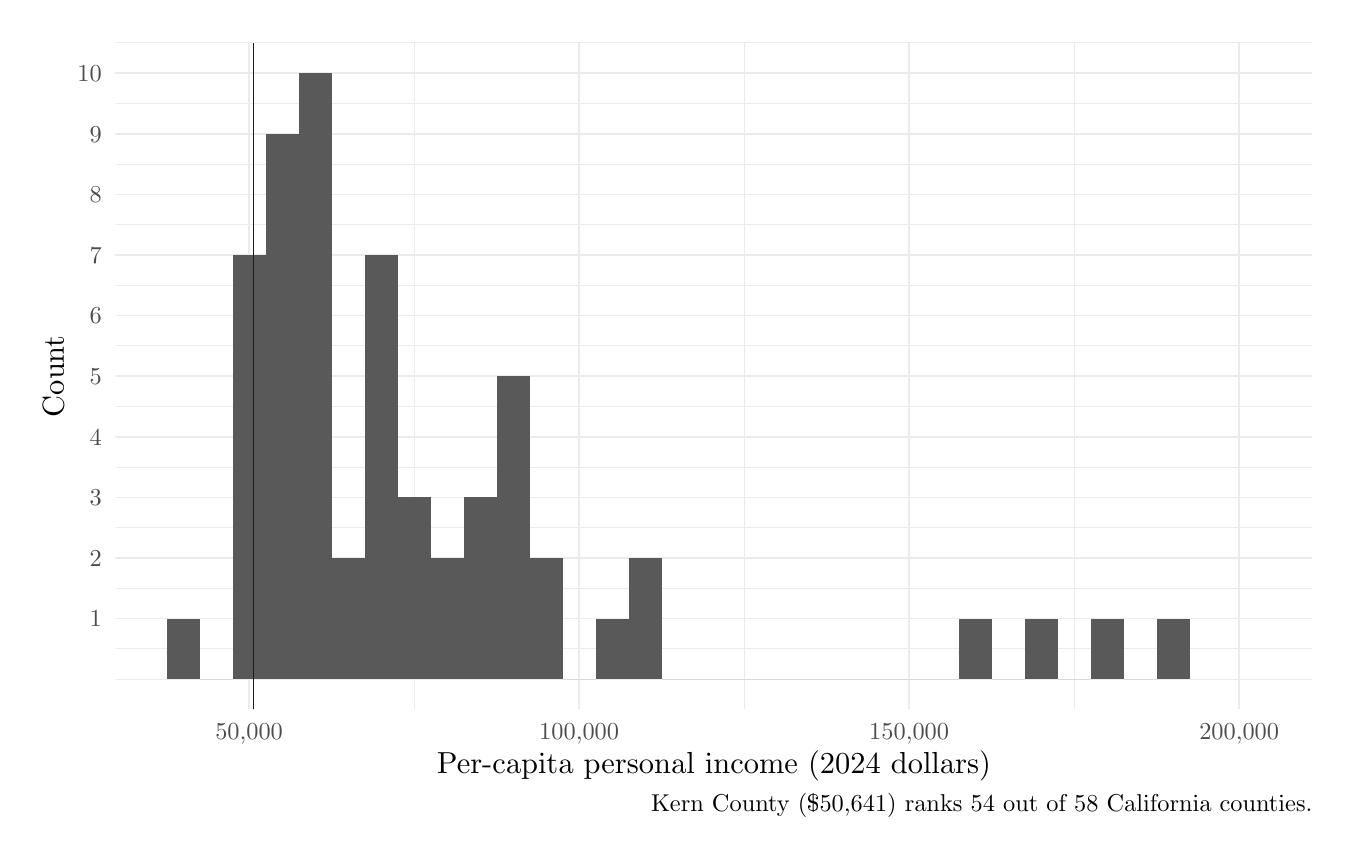
\begin{tikzpicture}[x=1pt,y=1pt]
\definecolor{fillColor}{RGB}{255,255,255}
\path[use as bounding box,fill=fillColor,fill opacity=0.00] (0,0) rectangle (469.75,290.32);
\begin{scope}
\path[clip] (  0.00,  0.00) rectangle (469.75,290.32);
\definecolor{fillColor}{RGB}{255,255,255}

\path[fill=fillColor] (  0.00,  0.00) rectangle (469.76,290.32);
\end{scope}
\begin{scope}
\path[clip] ( 31.71, 43.96) rectangle (464.25,284.82);
\definecolor{drawColor}{gray}{0.92}

\path[draw=drawColor,line width= 0.3pt,line join=round] ( 31.71, 54.91) --
	(464.25, 54.91);

\path[draw=drawColor,line width= 0.3pt,line join=round] ( 31.71, 65.85) --
	(464.25, 65.85);

\path[draw=drawColor,line width= 0.3pt,line join=round] ( 31.71, 87.75) --
	(464.25, 87.75);

\path[draw=drawColor,line width= 0.3pt,line join=round] ( 31.71,109.65) --
	(464.25,109.65);

\path[draw=drawColor,line width= 0.3pt,line join=round] ( 31.71,131.55) --
	(464.25,131.55);

\path[draw=drawColor,line width= 0.3pt,line join=round] ( 31.71,153.44) --
	(464.25,153.44);

\path[draw=drawColor,line width= 0.3pt,line join=round] ( 31.71,175.34) --
	(464.25,175.34);

\path[draw=drawColor,line width= 0.3pt,line join=round] ( 31.71,197.24) --
	(464.25,197.24);

\path[draw=drawColor,line width= 0.3pt,line join=round] ( 31.71,219.13) --
	(464.25,219.13);

\path[draw=drawColor,line width= 0.3pt,line join=round] ( 31.71,241.03) --
	(464.25,241.03);

\path[draw=drawColor,line width= 0.3pt,line join=round] ( 31.71,262.93) --
	(464.25,262.93);

\path[draw=drawColor,line width= 0.3pt,line join=round] ( 31.71,284.82) --
	(464.25,284.82);

\path[draw=drawColor,line width= 0.3pt,line join=round] (139.64, 43.96) --
	(139.64,284.82);

\path[draw=drawColor,line width= 0.3pt,line join=round] (258.90, 43.96) --
	(258.90,284.82);

\path[draw=drawColor,line width= 0.3pt,line join=round] (378.15, 43.96) --
	(378.15,284.82);

\path[draw=drawColor,line width= 0.6pt,line join=round] ( 31.71, 76.80) --
	(464.25, 76.80);

\path[draw=drawColor,line width= 0.6pt,line join=round] ( 31.71, 98.70) --
	(464.25, 98.70);

\path[draw=drawColor,line width= 0.6pt,line join=round] ( 31.71,120.60) --
	(464.25,120.60);

\path[draw=drawColor,line width= 0.6pt,line join=round] ( 31.71,142.49) --
	(464.25,142.49);

\path[draw=drawColor,line width= 0.6pt,line join=round] ( 31.71,164.39) --
	(464.25,164.39);

\path[draw=drawColor,line width= 0.6pt,line join=round] ( 31.71,186.29) --
	(464.25,186.29);

\path[draw=drawColor,line width= 0.6pt,line join=round] ( 31.71,208.18) --
	(464.25,208.18);

\path[draw=drawColor,line width= 0.6pt,line join=round] ( 31.71,230.08) --
	(464.25,230.08);

\path[draw=drawColor,line width= 0.6pt,line join=round] ( 31.71,251.98) --
	(464.25,251.98);

\path[draw=drawColor,line width= 0.6pt,line join=round] ( 31.71,273.88) --
	(464.25,273.88);

\path[draw=drawColor,line width= 0.6pt,line join=round] ( 80.01, 43.96) --
	( 80.01,284.82);

\path[draw=drawColor,line width= 0.6pt,line join=round] (199.27, 43.96) --
	(199.27,284.82);

\path[draw=drawColor,line width= 0.6pt,line join=round] (318.52, 43.96) --
	(318.52,284.82);

\path[draw=drawColor,line width= 0.6pt,line join=round] (437.78, 43.96) --
	(437.78,284.82);
\definecolor{fillColor}{gray}{0.35}

\path[fill=fillColor] ( 50.20, 54.91) rectangle ( 62.12, 76.80);

\path[fill=fillColor] ( 62.12, 54.91) rectangle ( 74.05, 54.91);

\path[fill=fillColor] ( 74.05, 54.91) rectangle ( 85.97,208.18);

\path[fill=fillColor] ( 85.97, 54.91) rectangle ( 97.90,251.98);

\path[fill=fillColor] ( 97.90, 54.91) rectangle (109.83,273.88);

\path[fill=fillColor] (109.83, 54.91) rectangle (121.75, 98.70);

\path[fill=fillColor] (121.75, 54.91) rectangle (133.68,208.18);

\path[fill=fillColor] (133.68, 54.91) rectangle (145.60,120.60);

\path[fill=fillColor] (145.60, 54.91) rectangle (157.53, 98.70);

\path[fill=fillColor] (157.53, 54.91) rectangle (169.45,120.60);

\path[fill=fillColor] (169.45, 54.91) rectangle (181.38,164.39);

\path[fill=fillColor] (181.38, 54.91) rectangle (193.30, 98.70);

\path[fill=fillColor] (193.30, 54.91) rectangle (205.23, 54.91);

\path[fill=fillColor] (205.23, 54.91) rectangle (217.16, 76.80);

\path[fill=fillColor] (217.16, 54.91) rectangle (229.08, 98.70);

\path[fill=fillColor] (229.08, 54.91) rectangle (241.01, 54.91);

\path[fill=fillColor] (241.01, 54.91) rectangle (252.93, 54.91);

\path[fill=fillColor] (252.93, 54.91) rectangle (264.86, 54.91);

\path[fill=fillColor] (264.86, 54.91) rectangle (276.78, 54.91);

\path[fill=fillColor] (276.78, 54.91) rectangle (288.71, 54.91);

\path[fill=fillColor] (288.71, 54.91) rectangle (300.64, 54.91);

\path[fill=fillColor] (300.64, 54.91) rectangle (312.56, 54.91);

\path[fill=fillColor] (312.56, 54.91) rectangle (324.49, 54.91);

\path[fill=fillColor] (324.49, 54.91) rectangle (336.41, 54.91);

\path[fill=fillColor] (336.41, 54.91) rectangle (348.34, 76.80);

\path[fill=fillColor] (348.34, 54.91) rectangle (360.26, 54.91);

\path[fill=fillColor] (360.26, 54.91) rectangle (372.19, 76.80);

\path[fill=fillColor] (372.19, 54.91) rectangle (384.11, 54.91);

\path[fill=fillColor] (384.11, 54.91) rectangle (396.04, 76.80);

\path[fill=fillColor] (396.04, 54.91) rectangle (407.97, 54.91);

\path[fill=fillColor] (407.97, 54.91) rectangle (419.89, 76.80);
\definecolor{drawColor}{RGB}{0,26,112}

\path[draw=drawColor,line width= 0.6pt,line join=round] ( 81.54, 43.96) -- ( 81.54,284.82);
\end{scope}
\begin{scope}
\path[clip] (  0.00,  0.00) rectangle (469.75,290.32);
\definecolor{drawColor}{gray}{0.30}

\node[text=drawColor,anchor=base east,inner sep=0pt, outer sep=0pt, scale=  0.88] at ( 26.76, 73.77) {1};

\node[text=drawColor,anchor=base east,inner sep=0pt, outer sep=0pt, scale=  0.88] at ( 26.76, 95.67) {2};

\node[text=drawColor,anchor=base east,inner sep=0pt, outer sep=0pt, scale=  0.88] at ( 26.76,117.57) {3};

\node[text=drawColor,anchor=base east,inner sep=0pt, outer sep=0pt, scale=  0.88] at ( 26.76,139.46) {4};

\node[text=drawColor,anchor=base east,inner sep=0pt, outer sep=0pt, scale=  0.88] at ( 26.76,161.36) {5};

\node[text=drawColor,anchor=base east,inner sep=0pt, outer sep=0pt, scale=  0.88] at ( 26.76,183.26) {6};

\node[text=drawColor,anchor=base east,inner sep=0pt, outer sep=0pt, scale=  0.88] at ( 26.76,205.15) {7};

\node[text=drawColor,anchor=base east,inner sep=0pt, outer sep=0pt, scale=  0.88] at ( 26.76,227.05) {8};

\node[text=drawColor,anchor=base east,inner sep=0pt, outer sep=0pt, scale=  0.88] at ( 26.76,248.95) {9};

\node[text=drawColor,anchor=base east,inner sep=0pt, outer sep=0pt, scale=  0.88] at ( 26.76,270.85) {10};
\end{scope}
\begin{scope}
\path[clip] (  0.00,  0.00) rectangle (469.75,290.32);
\definecolor{drawColor}{gray}{0.30}

\node[text=drawColor,anchor=base,inner sep=0pt, outer sep=0pt, scale=  0.88] at ( 80.01, 32.95) {50,000};

\node[text=drawColor,anchor=base,inner sep=0pt, outer sep=0pt, scale=  0.88] at (199.27, 32.95) {100,000};

\node[text=drawColor,anchor=base,inner sep=0pt, outer sep=0pt, scale=  0.88] at (318.52, 32.95) {150,000};

\node[text=drawColor,anchor=base,inner sep=0pt, outer sep=0pt, scale=  0.88] at (437.78, 32.95) {200,000};
\end{scope}
\begin{scope}
\path[clip] (  0.00,  0.00) rectangle (469.75,290.32);
\definecolor{drawColor}{RGB}{0,0,0}

\node[text=drawColor,anchor=base,inner sep=0pt, outer sep=0pt, scale=  1.10] at (247.98, 20.91) {Per-capita personal income (2024 dollars)};
\end{scope}
\begin{scope}
\path[clip] (  0.00,  0.00) rectangle (469.75,290.32);
\definecolor{drawColor}{RGB}{0,0,0}

\node[text=drawColor,rotate= 90.00,anchor=base,inner sep=0pt, outer sep=0pt, scale=  1.10] at ( 13.08,164.39) {Count};
\end{scope}
\begin{scope}
\path[clip] (  0.00,  0.00) rectangle (469.75,290.32);
\definecolor{drawColor}{RGB}{0,0,0}

\node[text=drawColor,anchor=base east,inner sep=0pt, outer sep=0pt, scale=  0.88] at (464.25,  7.21) {Kern County (\$50,641) ranks 54 out of 58 California counties.};
\end{scope}
\end{tikzpicture}
}  
  \caption{Summary of per-capita personal income across California counties}
\end{figure}

\begin{figure}[htbp]
  \centering
  \resizebox{\textwidth}{!}{
  % Created by tikzDevice version 0.12.6 on 2026-05-29 08:00:36
% !TEX encoding = UTF-8 Unicode
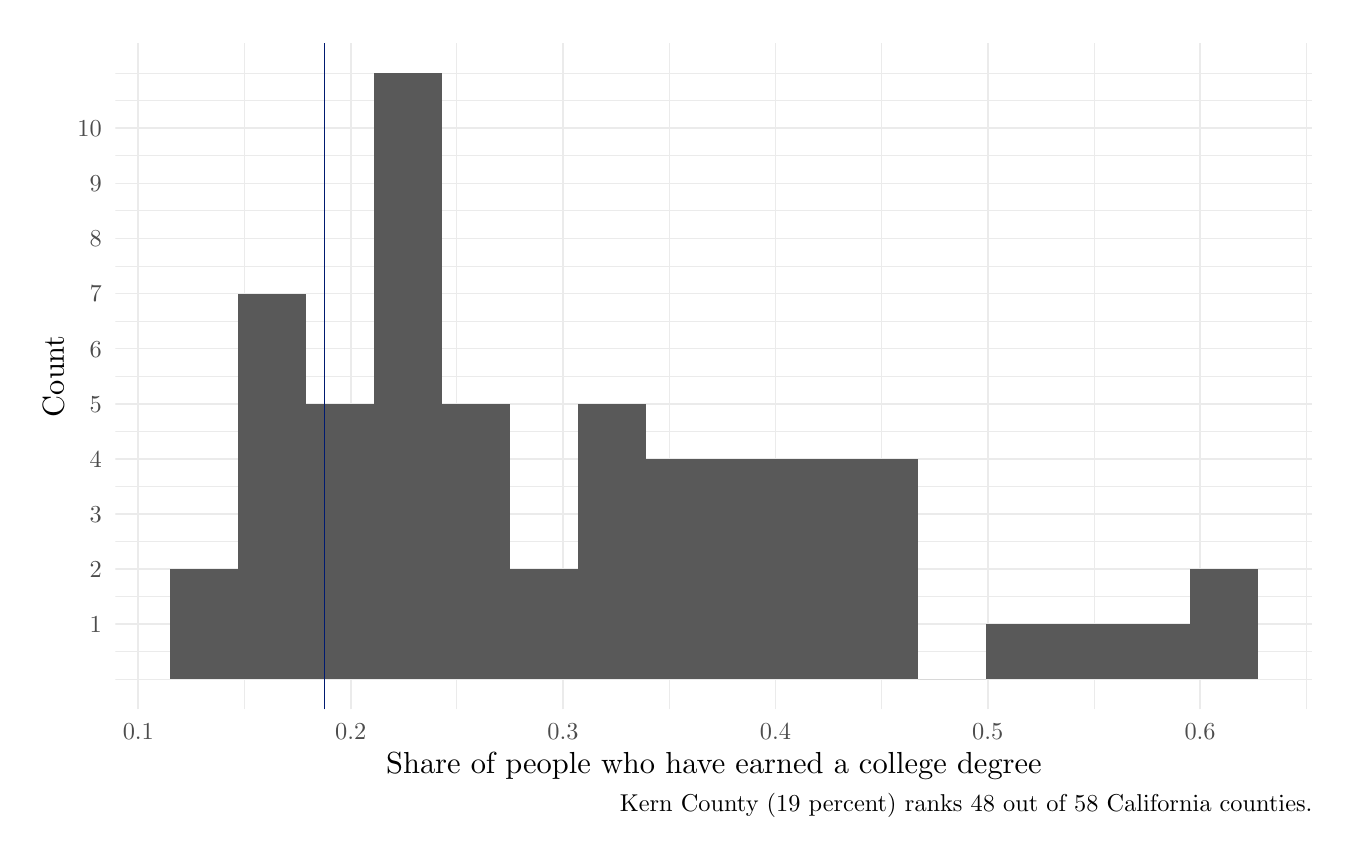
\begin{tikzpicture}[x=1pt,y=1pt]
\definecolor{fillColor}{RGB}{255,255,255}
\path[use as bounding box,fill=fillColor,fill opacity=0.00] (0,0) rectangle (469.75,290.32);
\begin{scope}
\path[clip] (  0.00,  0.00) rectangle (469.75,290.32);
\definecolor{fillColor}{RGB}{255,255,255}

\path[fill=fillColor] (  0.00,  0.00) rectangle (469.76,290.32);
\end{scope}
\begin{scope}
\path[clip] ( 31.71, 43.96) rectangle (464.25,284.82);
\definecolor{drawColor}{gray}{0.92}

\path[draw=drawColor,line width= 0.3pt,line join=round] ( 31.71, 54.91) --
	(464.25, 54.91);

\path[draw=drawColor,line width= 0.3pt,line join=round] ( 31.71, 64.86) --
	(464.25, 64.86);

\path[draw=drawColor,line width= 0.3pt,line join=round] ( 31.71, 84.77) --
	(464.25, 84.77);

\path[draw=drawColor,line width= 0.3pt,line join=round] ( 31.71,104.67) --
	(464.25,104.67);

\path[draw=drawColor,line width= 0.3pt,line join=round] ( 31.71,124.58) --
	(464.25,124.58);

\path[draw=drawColor,line width= 0.3pt,line join=round] ( 31.71,144.48) --
	(464.25,144.48);

\path[draw=drawColor,line width= 0.3pt,line join=round] ( 31.71,164.39) --
	(464.25,164.39);

\path[draw=drawColor,line width= 0.3pt,line join=round] ( 31.71,184.30) --
	(464.25,184.30);

\path[draw=drawColor,line width= 0.3pt,line join=round] ( 31.71,204.20) --
	(464.25,204.20);

\path[draw=drawColor,line width= 0.3pt,line join=round] ( 31.71,224.11) --
	(464.25,224.11);

\path[draw=drawColor,line width= 0.3pt,line join=round] ( 31.71,244.02) --
	(464.25,244.02);

\path[draw=drawColor,line width= 0.3pt,line join=round] ( 31.71,263.92) --
	(464.25,263.92);

\path[draw=drawColor,line width= 0.3pt,line join=round] ( 31.71,273.88) --
	(464.25,273.88);

\path[draw=drawColor,line width= 0.3pt,line join=round] ( 78.35, 43.96) --
	( 78.35,284.82);

\path[draw=drawColor,line width= 0.3pt,line join=round] (155.09, 43.96) --
	(155.09,284.82);

\path[draw=drawColor,line width= 0.3pt,line join=round] (231.82, 43.96) --
	(231.82,284.82);

\path[draw=drawColor,line width= 0.3pt,line join=round] (308.56, 43.96) --
	(308.56,284.82);

\path[draw=drawColor,line width= 0.3pt,line join=round] (385.29, 43.96) --
	(385.29,284.82);

\path[draw=drawColor,line width= 0.3pt,line join=round] (462.03, 43.96) --
	(462.03,284.82);

\path[draw=drawColor,line width= 0.6pt,line join=round] ( 31.71, 74.81) --
	(464.25, 74.81);

\path[draw=drawColor,line width= 0.6pt,line join=round] ( 31.71, 94.72) --
	(464.25, 94.72);

\path[draw=drawColor,line width= 0.6pt,line join=round] ( 31.71,114.62) --
	(464.25,114.62);

\path[draw=drawColor,line width= 0.6pt,line join=round] ( 31.71,134.53) --
	(464.25,134.53);

\path[draw=drawColor,line width= 0.6pt,line join=round] ( 31.71,154.44) --
	(464.25,154.44);

\path[draw=drawColor,line width= 0.6pt,line join=round] ( 31.71,174.34) --
	(464.25,174.34);

\path[draw=drawColor,line width= 0.6pt,line join=round] ( 31.71,194.25) --
	(464.25,194.25);

\path[draw=drawColor,line width= 0.6pt,line join=round] ( 31.71,214.16) --
	(464.25,214.16);

\path[draw=drawColor,line width= 0.6pt,line join=round] ( 31.71,234.06) --
	(464.25,234.06);

\path[draw=drawColor,line width= 0.6pt,line join=round] ( 31.71,253.97) --
	(464.25,253.97);

\path[draw=drawColor,line width= 0.6pt,line join=round] ( 39.98, 43.96) --
	( 39.98,284.82);

\path[draw=drawColor,line width= 0.6pt,line join=round] (116.72, 43.96) --
	(116.72,284.82);

\path[draw=drawColor,line width= 0.6pt,line join=round] (193.45, 43.96) --
	(193.45,284.82);

\path[draw=drawColor,line width= 0.6pt,line join=round] (270.19, 43.96) --
	(270.19,284.82);

\path[draw=drawColor,line width= 0.6pt,line join=round] (346.92, 43.96) --
	(346.92,284.82);

\path[draw=drawColor,line width= 0.6pt,line join=round] (423.66, 43.96) --
	(423.66,284.82);
\definecolor{fillColor}{gray}{0.35}

\path[fill=fillColor] ( 51.37, 54.91) rectangle ( 75.95, 94.72);

\path[fill=fillColor] ( 75.95, 54.91) rectangle (100.53,194.25);

\path[fill=fillColor] (100.53, 54.91) rectangle (125.10,154.44);

\path[fill=fillColor] (125.10, 54.91) rectangle (149.68,273.88);

\path[fill=fillColor] (149.68, 54.91) rectangle (174.25,154.44);

\path[fill=fillColor] (174.25, 54.91) rectangle (198.83, 94.72);

\path[fill=fillColor] (198.83, 54.91) rectangle (223.41,154.44);

\path[fill=fillColor] (223.41, 54.91) rectangle (247.98,134.53);

\path[fill=fillColor] (247.98, 54.91) rectangle (272.56,134.53);

\path[fill=fillColor] (272.56, 54.91) rectangle (297.14,134.53);

\path[fill=fillColor] (297.14, 54.91) rectangle (321.71,134.53);

\path[fill=fillColor] (321.71, 54.91) rectangle (346.29, 54.91);

\path[fill=fillColor] (346.29, 54.91) rectangle (370.87, 74.81);

\path[fill=fillColor] (370.87, 54.91) rectangle (395.44, 74.81);

\path[fill=fillColor] (395.44, 54.91) rectangle (420.02, 74.81);

\path[fill=fillColor] (420.02, 54.91) rectangle (444.59, 94.72);
\definecolor{drawColor}{RGB}{0,26,112}

\path[draw=drawColor,line width= 0.6pt,line join=round] (107.29, 43.96) -- (107.29,284.82);
\end{scope}
\begin{scope}
\path[clip] (  0.00,  0.00) rectangle (469.75,290.32);
\definecolor{drawColor}{gray}{0.30}

\node[text=drawColor,anchor=base east,inner sep=0pt, outer sep=0pt, scale=  0.88] at ( 26.76, 71.78) {1};

\node[text=drawColor,anchor=base east,inner sep=0pt, outer sep=0pt, scale=  0.88] at ( 26.76, 91.69) {2};

\node[text=drawColor,anchor=base east,inner sep=0pt, outer sep=0pt, scale=  0.88] at ( 26.76,111.59) {3};

\node[text=drawColor,anchor=base east,inner sep=0pt, outer sep=0pt, scale=  0.88] at ( 26.76,131.50) {4};

\node[text=drawColor,anchor=base east,inner sep=0pt, outer sep=0pt, scale=  0.88] at ( 26.76,151.41) {5};

\node[text=drawColor,anchor=base east,inner sep=0pt, outer sep=0pt, scale=  0.88] at ( 26.76,171.31) {6};

\node[text=drawColor,anchor=base east,inner sep=0pt, outer sep=0pt, scale=  0.88] at ( 26.76,191.22) {7};

\node[text=drawColor,anchor=base east,inner sep=0pt, outer sep=0pt, scale=  0.88] at ( 26.76,211.13) {8};

\node[text=drawColor,anchor=base east,inner sep=0pt, outer sep=0pt, scale=  0.88] at ( 26.76,231.03) {9};

\node[text=drawColor,anchor=base east,inner sep=0pt, outer sep=0pt, scale=  0.88] at ( 26.76,250.94) {10};
\end{scope}
\begin{scope}
\path[clip] (  0.00,  0.00) rectangle (469.75,290.32);
\definecolor{drawColor}{gray}{0.30}

\node[text=drawColor,anchor=base,inner sep=0pt, outer sep=0pt, scale=  0.88] at ( 39.98, 32.95) {0.1};

\node[text=drawColor,anchor=base,inner sep=0pt, outer sep=0pt, scale=  0.88] at (116.72, 32.95) {0.2};

\node[text=drawColor,anchor=base,inner sep=0pt, outer sep=0pt, scale=  0.88] at (193.45, 32.95) {0.3};

\node[text=drawColor,anchor=base,inner sep=0pt, outer sep=0pt, scale=  0.88] at (270.19, 32.95) {0.4};

\node[text=drawColor,anchor=base,inner sep=0pt, outer sep=0pt, scale=  0.88] at (346.92, 32.95) {0.5};

\node[text=drawColor,anchor=base,inner sep=0pt, outer sep=0pt, scale=  0.88] at (423.66, 32.95) {0.6};
\end{scope}
\begin{scope}
\path[clip] (  0.00,  0.00) rectangle (469.75,290.32);
\definecolor{drawColor}{RGB}{0,0,0}

\node[text=drawColor,anchor=base,inner sep=0pt, outer sep=0pt, scale=  1.10] at (247.98, 20.91) {Share of people who have earned a college degree};
\end{scope}
\begin{scope}
\path[clip] (  0.00,  0.00) rectangle (469.75,290.32);
\definecolor{drawColor}{RGB}{0,0,0}

\node[text=drawColor,rotate= 90.00,anchor=base,inner sep=0pt, outer sep=0pt, scale=  1.10] at ( 13.08,164.39) {Count};
\end{scope}
\begin{scope}
\path[clip] (  0.00,  0.00) rectangle (469.75,290.32);
\definecolor{drawColor}{RGB}{0,0,0}

\node[text=drawColor,anchor=base east,inner sep=0pt, outer sep=0pt, scale=  0.88] at (464.25,  7.21) {Kern County (19 percent) ranks 48 out of 58 California counties.};
\end{scope}
\end{tikzpicture}
}  
  \caption{Summary of educational attainment across California counties}
\end{figure}

\clearpage
\pagebreak

\section{Tables}

\begin{table}[h]
  \centering
  \caption{Counterfactual employment values, January $1997$ to December $2009$}
  \resizebox{\textwidth}{!}{
    
\begin{tabular}{lcrcrcr}
\toprule
\multicolumn{1}{c}{ } & \multicolumn{2}{c}{Jan 2000} & \multicolumn{2}{c}{Jan 2005} & \multicolumn{2}{c}{Dec 2009} \\
\cmidrule(l{3pt}r{3pt}){2-3} \cmidrule(l{3pt}r{3pt}){4-5} \cmidrule(l{3pt}r{3pt}){6-7}
Counterfactual & Employment & Percent & Employment & Percent & Employment & Percent\\
\midrule
\textbf{Employment data} & 235,843 & 0.0 & 255,850 & 0.0 & 261,364 & 0.0\\
Less oil-supply disruption & 235,262 & $-$0.2 & \textcolor{blue}{262,199} & \textcolor{blue}{2.5} & 264,295 & 1.1\\
Less agg demand & 236,395 & 0.2 & 250,021 & $-$2.3 & 257,162 & $-$1.6\\
Less oil-specific demand & \textcolor{blue}{237,678} & \textcolor{blue}{0.8} & 257,264 & 0.6 & 266,448 & 1.9\\
Less local shocks & 236,720 & 0.4 & 255,217 & $-$0.2 & \textcolor{blue}{272,749} & \textcolor{blue}{4.4}\\
\bottomrule
\end{tabular}
}
\end{table}

\begin{table}[h]
  \centering
  \caption{Counterfactual employment values, January 2010 to December 2024}
  \resizebox{\textwidth}{!}{
    
\begin{tabular}{lcrcrcr}
\toprule
\multicolumn{1}{c}{ } & \multicolumn{2}{c}{Jan 2015} & \multicolumn{2}{c}{Jan 2020} & \multicolumn{2}{c}{Dec 2024} \\
\cmidrule(l{3pt}r{3pt}){2-3} \cmidrule(l{3pt}r{3pt}){4-5} \cmidrule(l{3pt}r{3pt}){6-7}
Counterfactual & Employment & Percent & Employment & Percent & Employment & Percent\\
\midrule
\textbf{Employment data} & 312,895 & 0.0 & 336,413 & 0.0 & 341,302 & 0.0\\
Less oil-supply disruption & 310,722 & $-$0.7 & 333,852 & $-$0.8 & 336,496 & $-$1.4\\
Less agg demand & 316,792 & 1.2 & 340,904 & 1.3 & 344,700 & 1.0\\
Less oil-specific demand & \textcolor{blue}{295,484} & \textcolor{blue}{$-$5.6} & \textcolor{blue}{314,568} & \textcolor{blue}{$-$6.5} & \textcolor{blue}{323,992} & \textcolor{blue}{$-$5.1}\\
Less local shocks & 298,511 & $-$4.6 & 324,453 & $-$3.6 & 349,406 & 2.4\\
\bottomrule
\end{tabular}
}
\end{table}

\begin{table}

\caption{\label{tab:fevd-dempl} Forecast error variance decomposition for employment growth}
\centering
\begin{tabular}[t]{lllll}
\toprule
\multicolumn{1}{c}{ } & \multicolumn{4}{c}{Percent of $h$-step ahead forecast error variance explained by} \\
\cmidrule(l{3pt}r{3pt}){2-5}
\makecell[l]{\\Horizon} & \makecell[l]{Oil-supply\\shock} & \makecell[l]{Aggregate-\\demand shock} & \makecell[l]{Oil-specific-\\demand shock} & \makecell[l]{Residual\\shock}\\
\midrule
1 & 0.7 & 0.1 & 2.4 & 96.7\\
2 & 1.6 & 0.7 & 5.9 & 91.9\\
3 & 1.7 & 2.6 & 6.0 & 89.7\\
12 & 4.4 & 6.9 & 6.3 & 82.3\\
$\infty$ & 5.3 & 7.2 & 6.4 & 81.2\\
\bottomrule
\end{tabular}
\end{table}



\begin{table}

\caption{\label{tab:fevd-oilsupply} Forecast error variance decomposition for oil supply}
\centering
\begin{tabular}[t]{lllll}
\toprule
\multicolumn{1}{c}{ } & \multicolumn{4}{c}{Percent of $h$-step ahead forecast error variance explained by} \\
\cmidrule(l{3pt}r{3pt}){2-5}
\makecell[l]{\\Horizon} & \makecell[l]{Oil-supply\\shock} & \makecell[l]{Aggregate-\\demand shock} & \makecell[l]{Oil-specific-\\demand shock} & \makecell[l]{Residual\\shock}\\
\midrule
1 & 100.0 & 0.0 & 0.0 & 0.0\\
2 & 80.9 & 0.1 & 2.0 & 17.0\\
3 & 76.5 & 0.3 & 7.3 & 15.9\\
12 & 69.0 & 6.4 & 7.9 & 16.7\\
$\infty$ & 68.2 & 6.9 & 8.2 & 16.7\\
\bottomrule
\end{tabular}
\end{table}



\begin{table}

\caption{\label{tab:fevd-rpoil} Forecast error variance decomposition for the real price of crude oil}
\centering
\begin{tabular}[t]{lllll}
\toprule
\multicolumn{1}{c}{ } & \multicolumn{4}{c}{Percent of $h$-step ahead forecast error variance explained by} \\
\cmidrule(l{3pt}r{3pt}){2-5}
\makecell[l]{\\Horizon} & \makecell[l]{Oil-supply\\shock} & \makecell[l]{Aggregate-\\demand shock} & \makecell[l]{Oil-specific-\\demand shock} & \makecell[l]{Residual\\shock}\\
\midrule
1 & 1.7 & 1.3 & 97.1 & 0.0\\
2 & 1.3 & 3.4 & 94.6 & 0.7\\
3 & 1.1 & 6.6 & 90.0 & 2.3\\
12 & 5.3 & 14.2 & 76.1 & 4.4\\
$\infty$ & 9.7 & 26.2 & 56.0 & 8.0\\
\bottomrule
\end{tabular}
\end{table}


\end{document}

%%% Local Variables:
%%% TeX-master: t
%%% TeX-engine: xetex
%%% End:
